\chapter{Lược đồ E--R và mô tả dữ liệu}

\section{Phạm vi và nguồn mô tả}

Schema trong mã nguồn được quản lý bằng các migration SQL từ \texttt{001\_initial\_schema.sql} đến \texttt{027\_customer\_email\_activation.sql}. Data dictionary của dự án mô tả 70 bảng nghiệp vụ dựa trên schema MySQL test; bảng kỹ thuật \texttt{schema\_migrations} do migration runner tạo riêng. Nội dung dưới đây bám theo migration và data dictionary hiện có, không mô tả dữ liệu runtime chưa được kiểm tra.

\section{Lược đồ E--R quan niệm}

Sơ đồ quan niệm trong báo cáo giới hạn ở tám thực thể lõi: STORE, EMPLOYEE, CUSTOMER, ACCOUNT, MACHINE, USAGE\_SESSION, ACCOUNT\_TRANSACTION và INVOICE. Đây là phạm vi của hình quan niệm, không phải toàn bộ 70 bảng. Các phân hệ mở rộng được mô tả theo từng bảng ở phần sau; quan hệ vật lý chi tiết được lưu trong data dictionary và file DBML của dự án.

\begin{figure}[htbp]

  \centering

  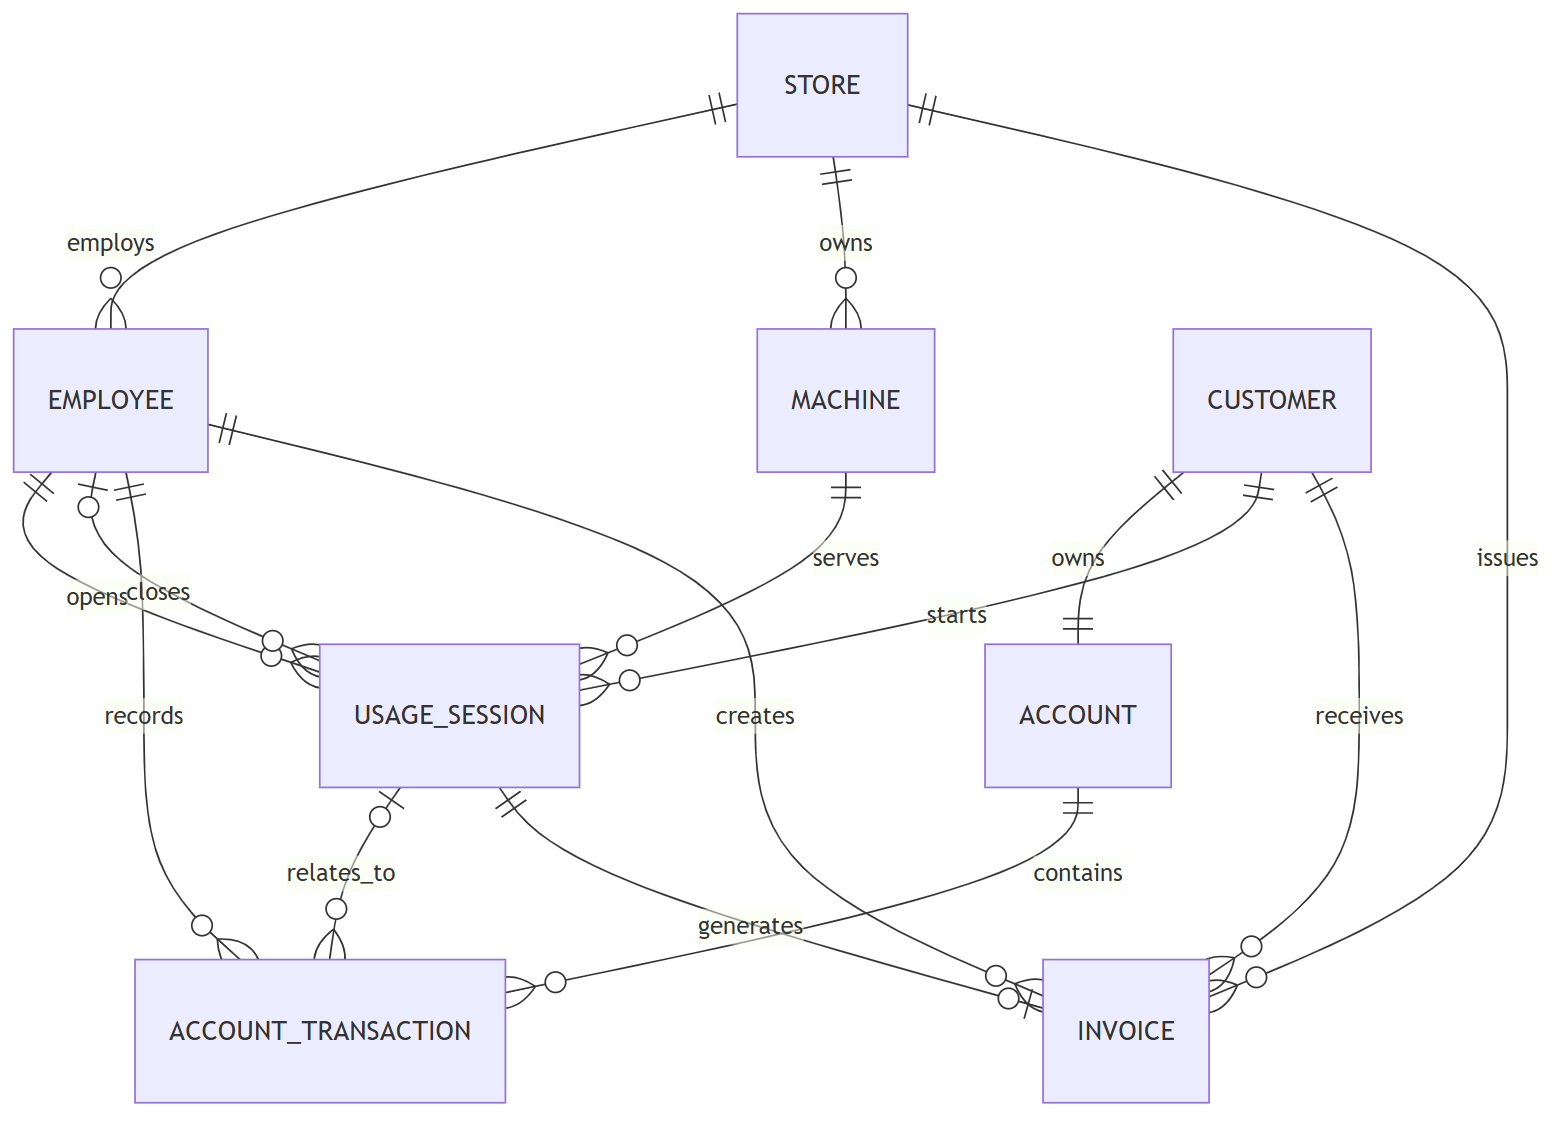
\includegraphics[width=0.98\textwidth,height=0.66\textheight,keepaspectratio]{figures/erd_conceptual.png}

  \caption{Mô hình E--R quan niệm của tám thực thể lõi}

  \label{fig:erd-core}

\end{figure}

\section{Mô tả các bảng theo phân hệ}

\subsection{Cửa hàng, nhân sự và kiểm toán}

\subsubsection{Bảng \texttt{stores}}

\textbf{Ý nghĩa:} Cửa hàng net. Nhân viên, máy và hóa đơn đều thuộc một cửa hàng.\par

\textbf{Thuộc tính:}

\begin{itemize}

\item \texttt{id} (\texttt{bigint unsigned}; PK; NOT NULL; AUTO_INCREMENT): Khóa chính.

\item \texttt{code} (\texttt{varchar(20)}; UK; NOT NULL): Mã cửa hàng, duy nhất.

\item \texttt{name} (\texttt{varchar(100)}; NOT NULL): Tên cửa hàng.

\item \texttt{address} (\texttt{varchar(255)}; NOT NULL): Địa chỉ.

\item \texttt{status} (\texttt{varchar(20)}; NOT NULL; mặc định \texttt{ACTIVE}): \texttt{ACTIVE} / \texttt{INACTIVE}. Cửa hàng ngừng hoạt động thì nhân viên không đăng nhập được.

\item \texttt{created\_at} (\texttt{datetime}; NOT NULL; mặc định \texttt{CURRENT\_TIMESTAMP}): Thời điểm tạo (UTC).

\item \texttt{updated\_at} (\texttt{datetime}; NOT NULL; mặc định \texttt{CURRENT\_TIMESTAMP}, tự cập nhật khi sửa): Thời điểm sửa gần nhất (UTC).

\end{itemize}

\textbf{Quan hệ:}

\begin{itemize}

\item Bảng con \texttt{employees}: FK \texttt{employees.store\_id} $\rightarrow$ \texttt{stores.id}; cardinality cha--con: 1 — 0..n. Cửa hàng nhân viên làm việc.

\item Bảng con \texttt{employee\_profiles}: FK \texttt{employee\_profiles.home\_store\_id} $\rightarrow$ \texttt{stores.id}; cardinality cha--con: 1 — 0..n. Cơ sở công tác chính.

\item Bảng con \texttt{employee\_store\_assignments}: FK \texttt{employee\_store\_assignments.store\_id} $\rightarrow$ \texttt{stores.id}; cardinality cha--con: 1 — 0..n. Cơ sở được phép vận hành; phần thứ hai của khóa chính.

\item Bảng con \texttt{customer\_store\_links}: FK \texttt{customer\_store\_links.store\_id} $\rightarrow$ \texttt{stores.id}; cardinality cha--con: 1 — 0..n. Cơ sở liên quan; phần thứ hai của khóa chính.

\item Bảng con \texttt{machines}: FK \texttt{machines.store\_id} $\rightarrow$ \texttt{stores.id}; cardinality cha--con: 1 — 0..n. Cửa hàng sở hữu máy.

\item Bảng con \texttt{account\_transactions}: FK \texttt{account\_transactions.store\_id} $\rightarrow$ \texttt{stores.id}; cardinality cha--con: 1 — 0..n. Cơ sở ghi nhận giao dịch tại thời điểm phát sinh.

\item Bảng con \texttt{invoices}: FK \texttt{invoices.store\_id} $\rightarrow$ \texttt{stores.id}; cardinality cha--con: 1 — 0..n. Cửa hàng; dùng cho báo cáo doanh thu.

\item Bảng con \texttt{promotions}: FK \texttt{promotions.store\_id} $\rightarrow$ \texttt{stores.id}; cardinality cha--con: 0..1 — 0..n. Cơ sở áp dụng; NULL = toàn hệ thống.

\item Bảng con \texttt{management\_audit}: FK \texttt{management\_audit.store\_id} $\rightarrow$ \texttt{stores.id}; cardinality cha--con: 1 — 0..n. Cơ sở đang vận hành.

\item Bảng con \texttt{menu\_categories}: FK \texttt{menu\_categories.store\_id} $\rightarrow$ \texttt{stores.id}; cardinality cha--con: 1 — 0..n. Cơ sở sở hữu nhóm món.

\item Bảng con \texttt{menu\_items}: FK \texttt{menu\_items.store\_id} $\rightarrow$ \texttt{stores.id}; cardinality cha--con: 1 — 0..n. Cơ sở bán món; menu khác nhau giữa các cơ sở.

\item Bảng con \texttt{menu\_orders}: FK \texttt{menu\_orders.store\_id} $\rightarrow$ \texttt{stores.id}; cardinality cha--con: 1 — 0..n. Cơ sở của máy đang dùng.

\item Bảng con \texttt{inventory\_ingredients}: FK \texttt{inventory\_ingredients.store\_id} $\rightarrow$ \texttt{stores.id}; cardinality cha--con: 1 — 0..n. Cửa hàng sở hữu nguyên liệu; cùng \texttt{id} tạo khóa tham chiếu ghép cho sổ kho.

\item Bảng con \texttt{customer\_notification\_events}: FK \texttt{customer\_notification\_events.store\_id} $\rightarrow$ \texttt{stores.id}; cardinality cha--con: 1 — 0..n. Cửa hàng phát sinh thông báo.

\item Bảng con \texttt{pos\_order\_reversals}: FK \texttt{pos\_order\_reversals.store\_id} $\rightarrow$ \texttt{stores.id}; cardinality cha--con: 1 — 0..n. Cơ sở xử lý.

\item Bảng con \texttt{menu\_promotions}: FK \texttt{menu\_promotions.store\_id} $\rightarrow$ \texttt{stores.id}; cardinality cha--con: 1 — 0..n. Cơ sở áp dụng.

\item Bảng con \texttt{reward\_catalog}: FK \texttt{reward\_catalog.store\_id} $\rightarrow$ \texttt{stores.id}; cardinality cha--con: 0..1 — 0..n. Cơ sở áp dụng; NULL = mọi cơ sở (chỉ ADMIN tạo).

\item Bảng con \texttt{customer\_vouchers}: FK \texttt{customer\_vouchers.store\_id} $\rightarrow$ \texttt{stores.id}; cardinality cha--con: 0..1 — 0..n. Cơ sở áp dụng (chụp từ danh mục); NULL = mọi cơ sở.

\item Bảng con \texttt{customer\_vouchers}: FK \texttt{customer\_vouchers.used\_store\_id} $\rightarrow$ \texttt{stores.id}; cardinality cha--con: 0..1 — 0..n. Cơ sở nơi dùng.

\item Bảng con \texttt{voucher\_events}: FK \texttt{voucher\_events.store\_id} $\rightarrow$ \texttt{stores.id}; cardinality cha--con: 0..1 — 0..n. Cơ sở phát sinh.

\item Bảng con \texttt{cash\_shifts}: FK \texttt{cash\_shifts.store\_id} $\rightarrow$ \texttt{stores.id}; cardinality cha--con: 1 — 0..n. Cơ sở mở ca.

\item Bảng con \texttt{cash\_shift\_entries}: FK \texttt{cash\_shift\_entries.store\_id} $\rightarrow$ \texttt{stores.id}; cardinality cha--con: 1 — 0..n. Cơ sở phát sinh.

\item Bảng con \texttt{machine\_incidents}: FK \texttt{machine\_incidents.store\_id} $\rightarrow$ \texttt{stores.id}; cardinality cha--con: 1 — 0..n. Cơ sở có máy lỗi.

\item Bảng con \texttt{suppliers}: FK \texttt{suppliers.store\_id} $\rightarrow$ \texttt{stores.id}; cardinality cha--con: 1 — 0..n. Cơ sở quản lý nhà cung cấp.

\item Bảng con \texttt{purchase\_requests}: FK \texttt{purchase\_requests.store\_id} $\rightarrow$ \texttt{stores.id}; cardinality cha--con: 1 — 0..n. Cơ sở đề nghị.

\item Bảng con \texttt{purchase\_orders}: FK \texttt{purchase\_orders.store\_id} $\rightarrow$ \texttt{stores.id}; cardinality cha--con: 1 — 0..n. Cơ sở mua.

\item Bảng con \texttt{goods\_receipts}: FK \texttt{goods\_receipts.store\_id} $\rightarrow$ \texttt{stores.id}; cardinality cha--con: 1 — 0..n. Cơ sở nhận.

\item Bảng con \texttt{supplier\_payables}: FK \texttt{supplier\_payables.store\_id} $\rightarrow$ \texttt{stores.id}; cardinality cha--con: 1 — 0..n. Cơ sở chịu công nợ.

\item Bảng con \texttt{commercial\_placements}: FK \texttt{commercial\_placements.store\_id} $\rightarrow$ \texttt{stores.id}; cardinality cha--con: 0..1 — 0..n. Cửa hàng áp dụng; NULL = toàn hệ thống.

\item Bảng con \texttt{customer\_security\_audit}: FK \texttt{customer\_security\_audit.store\_id} $\rightarrow$ \texttt{stores.id}; cardinality cha--con: 0..1 — 0..n. Cơ sở liên quan nếu có; NULL với luồng web tự phục vụ.

\end{itemize}

\textbf{Ràng buộc và chỉ mục trong schema:}

\begin{itemize}

\item PRIMARY KEY (\texttt{id})

\item UNIQUE \texttt{uq\_stores\_code} (\texttt{code})

\item CHECK \texttt{chk\_stores\_address\_not\_blank}: \texttt{(char\_length(trim(address)) > 0)}

\item CHECK \texttt{chk\_stores\_code\_not\_blank}: \texttt{(char\_length(trim(code)) > 0)}

\item CHECK \texttt{chk\_stores\_name\_not\_blank}: \texttt{(char\_length(trim(name)) > 0)}

\item CHECK \texttt{chk\_stores\_status}: \texttt{(status in ('ACTIVE','INACTIVE'))}

\end{itemize}

\subsubsection{Bảng \texttt{employees}}

\textbf{Ý nghĩa:} Nhân viên đăng nhập ứng dụng; vai trò quyết định quyền thao tác.\par

\textbf{Thuộc tính:}

\begin{itemize}

\item \texttt{id} (\texttt{bigint unsigned}; PK; NOT NULL; AUTO_INCREMENT): Khóa chính.

\item \texttt{code} (\texttt{varchar(20)}; UK; NOT NULL): Mã nhân viên, duy nhất.

\item \texttt{store\_id} (\texttt{bigint unsigned}; FK $\rightarrow$ \texttt{stores.id}; NOT NULL): Cửa hàng nhân viên làm việc.

\item \texttt{full\_name} (\texttt{varchar(100)}; NOT NULL): Họ tên.

\item \texttt{username} (\texttt{varchar(30)}; UK; NOT NULL): Tên đăng nhập, duy nhất, 4–30 ký tự.

\item \texttt{password\_hash} (\texttt{varchar(255)}; NOT NULL): Mật khẩu đã băm bcrypt; không bao giờ trả ra UI/DTO.

\item \texttt{role} (\texttt{varchar(20)}; NOT NULL): \texttt{ADMIN} / \texttt{DIRECTOR} / \texttt{MANAGER} / \texttt{STAFF} / \texttt{KITCHEN} / \texttt{INVENTORY}; backend cấp quyền tối thiểu theo từng thao tác.

\item \texttt{status} (\texttt{varchar(20)}; NOT NULL; mặc định \texttt{ACTIVE}): \texttt{ACTIVE} / \texttt{INACTIVE} / \texttt{LOCKED}. Chỉ ACTIVE đăng nhập được.

\item \texttt{created\_at} (\texttt{datetime}; NOT NULL; mặc định \texttt{CURRENT\_TIMESTAMP}): Thời điểm tạo (UTC).

\item \texttt{updated\_at} (\texttt{datetime}; NOT NULL; mặc định \texttt{CURRENT\_TIMESTAMP}, tự cập nhật khi sửa): Thời điểm sửa gần nhất (UTC).

\item \texttt{auth\_version} (\texttt{int unsigned}; NOT NULL; mặc định \texttt{0}): Phiên bản xác thực; tăng khi đổi/đặt lại mật khẩu để thu hồi phiên cũ.

\item \texttt{must\_change\_password} (\texttt{tinyint(1)}; NOT NULL; mặc định \texttt{0}): TRUE khi tài khoản đang dùng mật khẩu tạm và phải đổi trước khi thao tác.

\item \texttt{password\_changed\_at} (\texttt{datetime}; NULL): Thời điểm đổi hoặc đặt lại mật khẩu gần nhất (UTC), có thể NULL với dữ liệu cũ.

\end{itemize}

\textbf{Quan hệ:}

\begin{itemize}

\item FK \texttt{employees.store\_id} $\rightarrow$ \texttt{stores.id}. Cardinality cha--con: 1 — 0..n. Cửa hàng nhân viên làm việc.

\item Bảng con \texttt{employee\_profiles}: FK \texttt{employee\_profiles.employee\_id} $\rightarrow$ \texttt{employees.id}; cardinality cha--con: 0..1 — 0..1. Tài khoản nhân viên được gắn; NULL khi mới tạo hồ sơ, UNIQUE khi đã cấp tài khoản.

\item Bảng con \texttt{employee\_store\_assignments}: FK \texttt{employee\_store\_assignments.employee\_id} $\rightarrow$ \texttt{employees.id}; cardinality cha--con: 1 — 0..n. Nhân viên được phân công; phần thứ nhất của khóa chính.

\item Bảng con \texttt{employee\_store\_assignments}: FK \texttt{employee\_store\_assignments.granted\_by} $\rightarrow$ \texttt{employees.id}; cardinality cha--con: 1 — 0..n. ADMIN đã cấp quyền phân công.

\item Bảng con \texttt{usage\_sessions}: FK \texttt{usage\_sessions.closed\_by} $\rightarrow$ \texttt{employees.id}; cardinality cha--con: 0..1 — 0..n. Nhân viên checkout; NULL khi phiên đang chạy.

\item Bảng con \texttt{usage\_sessions}: FK \texttt{usage\_sessions.opened\_by} $\rightarrow$ \texttt{employees.id}; cardinality cha--con: 1 — 0..n. Nhân viên mở phiên.

\item Bảng con \texttt{account\_transactions}: FK \texttt{account\_transactions.employee\_id} $\rightarrow$ \texttt{employees.id}; cardinality cha--con: 1 — 0..n. Nhân viên thực hiện.

\item Bảng con \texttt{invoices}: FK \texttt{invoices.employee\_id} $\rightarrow$ \texttt{employees.id}; cardinality cha--con: 1 — 0..n. Nhân viên checkout.

\item Bảng con \texttt{management\_audit}: FK \texttt{management\_audit.employee\_id} $\rightarrow$ \texttt{employees.id}; cardinality cha--con: 1 — 0..n. Nhân viên thực hiện.

\item Bảng con \texttt{menu\_item\_changes}: FK \texttt{menu\_item\_changes.employee\_id} $\rightarrow$ \texttt{employees.id}; cardinality cha--con: 1 — 0..n. Nhân viên thực hiện.

\item Bảng con \texttt{menu\_orders}: FK \texttt{menu\_orders.handled\_by} $\rightarrow$ \texttt{employees.id}; cardinality cha--con: 0..1 — 0..n. Nhân viên tiếp nhận/phục vụ/hủy; NULL khi còn NEW.

\item Bảng con \texttt{menu\_orders}: FK \texttt{menu\_orders.paid\_by} $\rightarrow$ \texttt{employees.id}; cardinality cha--con: 0..1 — 0..n. Nhân viên xác nhận thanh toán.

\item Bảng con \texttt{inventory\_movements}: FK \texttt{inventory\_movements.employee\_id} $\rightarrow$ \texttt{employees.id}; cardinality cha--con: 0..1 — 0..n. Nhân viên thực hiện hoặc phê duyệt; NULL với tác vụ hệ thống.

\item Bảng con \texttt{inventory\_counts}: FK \texttt{inventory\_counts.decided\_by} $\rightarrow$ \texttt{employees.id}; cardinality cha--con: 0..1 — 0..n. Nhân viên khác phê duyệt/từ chối; NULL khi đang chờ.

\item Bảng con \texttt{inventory\_counts}: FK \texttt{inventory\_counts.proposed\_by} $\rightarrow$ \texttt{employees.id}; cardinality cha--con: 1 — 0..n. Nhân viên đề xuất kiểm kê.

\item Bảng con \texttt{pos\_order\_reversals}: FK \texttt{pos\_order\_reversals.decided\_by} $\rightarrow$ \texttt{employees.id}; cardinality cha--con: 0..1 — 0..n. Quản lý quyết định; NULL khi đang chờ.

\item Bảng con \texttt{pos\_order\_reversals}: FK \texttt{pos\_order\_reversals.requested\_by} $\rightarrow$ \texttt{employees.id}; cardinality cha--con: 1 — 0..n. Nhân viên đề nghị.

\item Bảng con \texttt{customer\_vouchers}: FK \texttt{customer\_vouchers.issued\_by} $\rightarrow$ \texttt{employees.id}; cardinality cha--con: 0..1 — 0..n. Nhân viên phát (NULL khi do hệ thống).

\item Bảng con \texttt{customer\_vouchers}: FK \texttt{customer\_vouchers.used\_by} $\rightarrow$ \texttt{employees.id}; cardinality cha--con: 0..1 — 0..n. Nhân viên xác nhận.

\item Bảng con \texttt{voucher\_events}: FK \texttt{voucher\_events.employee\_id} $\rightarrow$ \texttt{employees.id}; cardinality cha--con: 0..1 — 0..n. Nhân viên thực hiện.

\item Bảng con \texttt{loyalty\_point\_grants}: FK \texttt{loyalty\_point\_grants.employee\_id} $\rightarrow$ \texttt{employees.id}; cardinality cha--con: 1 — 0..n. Nhân viên xác nhận.

\item Bảng con \texttt{cash\_shifts}: FK \texttt{cash\_shifts.employee\_id} $\rightarrow$ \texttt{employees.id}; cardinality cha--con: 1 — 0..n. Nhân viên chịu trách nhiệm ca.

\item Bảng con \texttt{cash\_shifts}: FK \texttt{cash\_shifts.reviewed\_by} $\rightarrow$ \texttt{employees.id}; cardinality cha--con: 0..1 — 0..n. Quản lý duyệt chênh lệch.

\item Bảng con \texttt{cash\_shift\_entries}: FK \texttt{cash\_shift\_entries.employee\_id} $\rightarrow$ \texttt{employees.id}; cardinality cha--con: 1 — 0..n. Nhân viên ghi nhận.

\item Bảng con \texttt{machine\_incidents}: FK \texttt{machine\_incidents.assigned\_to} $\rightarrow$ \texttt{employees.id}; cardinality cha--con: 0..1 — 0..n. Người được phân công; có thể NULL trước khi phân công.

\item Bảng con \texttt{machine\_incidents}: FK \texttt{machine\_incidents.reported\_by} $\rightarrow$ \texttt{employees.id}; cardinality cha--con: 1 — 0..n. Người báo lỗi.

\item Bảng con \texttt{machine\_incidents}: FK \texttt{machine\_incidents.verified\_by} $\rightarrow$ \texttt{employees.id}; cardinality cha--con: 0..1 — 0..n. Người nghiệm thu.

\item Bảng con \texttt{machine\_incident\_events}: FK \texttt{machine\_incident\_events.employee\_id} $\rightarrow$ \texttt{employees.id}; cardinality cha--con: 1 — 0..n. Người thực hiện.

\item Bảng con \texttt{purchase\_requests}: FK \texttt{purchase\_requests.decided\_by} $\rightarrow$ \texttt{employees.id}; cardinality cha--con: 0..1 — 0..n. Người duyệt/từ chối.

\item Bảng con \texttt{purchase\_requests}: FK \texttt{purchase\_requests.requested\_by} $\rightarrow$ \texttt{employees.id}; cardinality cha--con: 1 — 0..n. Người lập.

\item Bảng con \texttt{purchase\_orders}: FK \texttt{purchase\_orders.created\_by} $\rightarrow$ \texttt{employees.id}; cardinality cha--con: 1 — 0..n. Người tạo đơn.

\item Bảng con \texttt{goods\_receipts}: FK \texttt{goods\_receipts.received\_by} $\rightarrow$ \texttt{employees.id}; cardinality cha--con: 1 — 0..n. Người nhận.

\item Bảng con \texttt{supplier\_payables}: FK \texttt{supplier\_payables.paid\_by} $\rightarrow$ \texttt{employees.id}; cardinality cha--con: 0..1 — 0..n. Người thanh toán.

\item Bảng con \texttt{commercial\_contracts}: FK \texttt{commercial\_contracts.approved\_by} $\rightarrow$ \texttt{employees.id}; cardinality cha--con: 0..1 — 0..n. Người duyệt; phải khác người lập theo service.

\item Bảng con \texttt{commercial\_contracts}: FK \texttt{commercial\_contracts.created\_by} $\rightarrow$ \texttt{employees.id}; cardinality cha--con: 1 — 0..n. Nhân viên lập hợp đồng.

\item Bảng con \texttt{commercial\_campaigns}: FK \texttt{commercial\_campaigns.created\_by} $\rightarrow$ \texttt{employees.id}; cardinality cha--con: 1 — 0..n. Nhân viên tạo.

\item Bảng con \texttt{commercial\_settlements}: FK \texttt{commercial\_settlements.generated\_by} $\rightarrow$ \texttt{employees.id}; cardinality cha--con: 1 — 0..n. Nhân viên tạo kỳ.

\item Bảng con \texttt{commercial\_settlements}: FK \texttt{commercial\_settlements.reviewed\_by} $\rightarrow$ \texttt{employees.id}; cardinality cha--con: 0..1 — 0..n. Người duyệt, phải khác người tạo theo service.

\item Bảng con \texttt{supplier\_payable\_approvals}: FK \texttt{supplier\_payable\_approvals.approved\_by} $\rightarrow$ \texttt{employees.id}; cardinality cha--con: 1 — 0..n. Nhân viên phê duyệt, phải khác người thanh toán theo service trong chính sách tách quyền.

\item Bảng con \texttt{customer\_security\_audit}: FK \texttt{customer\_security\_audit.employee\_id} $\rightarrow$ \texttt{employees.id}; cardinality cha--con: 0..1 — 0..n. Nhân viên liên quan nếu thao tác tại quầy; NULL với luồng email tự phục vụ.

\end{itemize}

\textbf{Ràng buộc và chỉ mục trong schema:}

\begin{itemize}

\item PRIMARY KEY (\texttt{id})

\item UNIQUE \texttt{uq\_employees\_code} (\texttt{code})

\item UNIQUE \texttt{uq\_employees\_username} (\texttt{username})

\item FOREIGN KEY \texttt{fk\_employees\_store} (\texttt{store\_id}) $\rightarrow$ \texttt{stores} (\texttt{id}) ON UPDATE RESTRICT ON DELETE RESTRICT

\item CHECK \texttt{chk\_employees\_code\_not\_blank}: \texttt{(char\_length(trim(code)) > 0)}

\item CHECK \texttt{chk\_employees\_full\_name\_not\_blank}: \texttt{(char\_length(trim(full\_name)) > 0)}

\item CHECK \texttt{chk\_employees\_password\_hash\_not\_blank}: \texttt{(char\_length(trim(password\_hash)) > 0)}

\item CHECK \texttt{chk\_employees\_role}: \texttt{(role in ('ADMIN','DIRECTOR','MANAGER','STAFF','KITCHEN','INVENTORY'))}

\item CHECK \texttt{chk\_employees\_status}: \texttt{(status in ('ACTIVE','INACTIVE','LOCKED'))}

\item CHECK \texttt{chk\_employees\_username\_length}: \texttt{(char\_length(username) between 4 and 30)}

\item INDEX \texttt{idx\_employees\_store\_status} (\texttt{store\_id, status})

\end{itemize}

\subsubsection{Bảng \texttt{employee\_profiles}}

\textbf{Ý nghĩa:} Hồ sơ nhân sự độc lập với thông tin xác thực; DIRECTOR/MANAGER quản lý nghiệp vụ, ADMIN chỉ gắn/cấp tài khoản.\par

\textbf{Thuộc tính:}

\begin{itemize}

\item \texttt{id} (\texttt{bigint unsigned}; PK; NOT NULL; AUTO_INCREMENT): Khóa chính.

\item \texttt{employee\_id} (\texttt{bigint unsigned}; UK, FK $\rightarrow$ \texttt{employees.id}; NULL): Tài khoản nhân viên được gắn; NULL khi mới tạo hồ sơ, UNIQUE khi đã cấp tài khoản.

\item \texttt{code} (\texttt{varchar(20)}; UK; NOT NULL): Mã hồ sơ nhân sự, duy nhất.

\item \texttt{home\_store\_id} (\texttt{bigint unsigned}; FK $\rightarrow$ \texttt{stores.id}; NOT NULL): Cơ sở công tác chính.

\item \texttt{full\_name} (\texttt{varchar(100)}; NOT NULL): Họ tên nhân sự.

\item \texttt{employment\_status} (\texttt{varchar(10)}; NOT NULL; mặc định \texttt{ACTIVE}): \texttt{ACTIVE} / \texttt{INACTIVE}, tách khỏi trạng thái khóa đăng nhập.

\item \texttt{created\_at} (\texttt{datetime}; NOT NULL; mặc định \texttt{CURRENT\_TIMESTAMP}): Thời điểm tạo (UTC).

\item \texttt{updated\_at} (\texttt{datetime}; NOT NULL; mặc định \texttt{CURRENT\_TIMESTAMP}, tự cập nhật khi sửa): Thời điểm sửa gần nhất (UTC).

\end{itemize}

\textbf{Quan hệ:}

\begin{itemize}

\item FK \texttt{employee\_profiles.home\_store\_id} $\rightarrow$ \texttt{stores.id}. Cardinality cha--con: 1 — 0..n. Cơ sở công tác chính.

\item FK \texttt{employee\_profiles.employee\_id} $\rightarrow$ \texttt{employees.id}. Cardinality cha--con: 0..1 — 0..1. Tài khoản nhân viên được gắn; NULL khi mới tạo hồ sơ, UNIQUE khi đã cấp tài khoản.

\end{itemize}

\textbf{Ràng buộc và chỉ mục trong schema:}

\begin{itemize}

\item PRIMARY KEY (\texttt{id})

\item UNIQUE \texttt{uq\_employee\_profiles\_code} (\texttt{code})

\item UNIQUE \texttt{uq\_employee\_profiles\_employee} (\texttt{employee\_id})

\item FOREIGN KEY \texttt{fk\_employee\_profiles\_employee} (\texttt{employee\_id}) $\rightarrow$ \texttt{employees} (\texttt{id}) ON UPDATE NO ACTION ON DELETE NO ACTION

\item FOREIGN KEY \texttt{fk\_employee\_profiles\_store} (\texttt{home\_store\_id}) $\rightarrow$ \texttt{stores} (\texttt{id}) ON UPDATE NO ACTION ON DELETE NO ACTION

\item CHECK \texttt{chk\_employee\_profiles\_status}: \texttt{(employment\_status in ('ACTIVE','INACTIVE'))}

\end{itemize}

\subsubsection{Bảng \texttt{employee\_store\_assignments}}

\textbf{Ý nghĩa:} Phân công bổ sung cho MANAGER được vận hành tại nhiều cơ sở; không thay đổi cơ sở chính trong hồ sơ.\par

\textbf{Thuộc tính:}

\begin{itemize}

\item \texttt{employee\_id} (\texttt{bigint unsigned}; PK, FK $\rightarrow$ \texttt{employees.id}; NOT NULL): Nhân viên được phân công; phần thứ nhất của khóa chính.

\item \texttt{store\_id} (\texttt{bigint unsigned}; PK, FK $\rightarrow$ \texttt{stores.id}; NOT NULL): Cơ sở được phép vận hành; phần thứ hai của khóa chính.

\item \texttt{granted\_by} (\texttt{bigint unsigned}; FK $\rightarrow$ \texttt{employees.id}; NOT NULL): ADMIN đã cấp quyền phân công.

\item \texttt{granted\_at} (\texttt{datetime}; NOT NULL; mặc định \texttt{CURRENT\_TIMESTAMP}): Thời điểm cấp (UTC).

\end{itemize}

\textbf{Quan hệ:}

\begin{itemize}

\item FK \texttt{employee\_store\_assignments.store\_id} $\rightarrow$ \texttt{stores.id}. Cardinality cha--con: 1 — 0..n. Cơ sở được phép vận hành; phần thứ hai của khóa chính.

\item FK \texttt{employee\_store\_assignments.employee\_id} $\rightarrow$ \texttt{employees.id}. Cardinality cha--con: 1 — 0..n. Nhân viên được phân công; phần thứ nhất của khóa chính.

\item FK \texttt{employee\_store\_assignments.granted\_by} $\rightarrow$ \texttt{employees.id}. Cardinality cha--con: 1 — 0..n. ADMIN đã cấp quyền phân công.

\end{itemize}

\textbf{Ràng buộc và chỉ mục trong schema:}

\begin{itemize}

\item PRIMARY KEY (\texttt{employee\_id,store\_id})

\item FOREIGN KEY \texttt{fk\_employee\_assignments\_employee} (\texttt{employee\_id}) $\rightarrow$ \texttt{employees} (\texttt{id}) ON UPDATE NO ACTION ON DELETE NO ACTION

\item FOREIGN KEY \texttt{fk\_employee\_assignments\_granter} (\texttt{granted\_by}) $\rightarrow$ \texttt{employees} (\texttt{id}) ON UPDATE NO ACTION ON DELETE NO ACTION

\item FOREIGN KEY \texttt{fk\_employee\_assignments\_store} (\texttt{store\_id}) $\rightarrow$ \texttt{stores} (\texttt{id}) ON UPDATE NO ACTION ON DELETE NO ACTION

\end{itemize}

\subsubsection{Bảng \texttt{management\_audit}}

\textbf{Ý nghĩa:} Lịch sử thay đổi quản trị, không lưu mật khẩu.\par

\textbf{Thuộc tính:}

\begin{itemize}

\item \texttt{id} (\texttt{bigint unsigned}; PK; NOT NULL; AUTO_INCREMENT): Khóa chính.

\item \texttt{employee\_id} (\texttt{bigint unsigned}; FK $\rightarrow$ \texttt{employees.id}; NOT NULL): Nhân viên thực hiện.

\item \texttt{store\_id} (\texttt{bigint unsigned}; FK $\rightarrow$ \texttt{stores.id}; NOT NULL): Cơ sở đang vận hành.

\item \texttt{action} (\texttt{varchar(40)}; NOT NULL): Loại thay đổi quản trị.

\item \texttt{entity\_id} (\texttt{bigint unsigned}; NOT NULL): ID đối tượng được thay đổi.

\item \texttt{created\_at} (\texttt{datetime}; NOT NULL; mặc định \texttt{CURRENT\_TIMESTAMP}): Thời điểm thay đổi (UTC).

\end{itemize}

\textbf{Quan hệ:}

\begin{itemize}

\item FK \texttt{management\_audit.store\_id} $\rightarrow$ \texttt{stores.id}. Cardinality cha--con: 1 — 0..n. Cơ sở đang vận hành.

\item FK \texttt{management\_audit.employee\_id} $\rightarrow$ \texttt{employees.id}. Cardinality cha--con: 1 — 0..n. Nhân viên thực hiện.

\end{itemize}

\textbf{Ràng buộc và chỉ mục trong schema:}

\begin{itemize}

\item PRIMARY KEY (\texttt{id})

\item FOREIGN KEY \texttt{fk\_management\_audit\_employee} (\texttt{employee\_id}) $\rightarrow$ \texttt{employees} (\texttt{id}) ON UPDATE NO ACTION ON DELETE RESTRICT

\item FOREIGN KEY \texttt{fk\_management\_audit\_store} (\texttt{store\_id}) $\rightarrow$ \texttt{stores} (\texttt{id}) ON UPDATE NO ACTION ON DELETE RESTRICT

\end{itemize}

\subsection{Khách hàng, tài khoản và bảo mật}

\subsubsection{Bảng \texttt{customers}}

\textbf{Ý nghĩa:} Thông tin cá nhân của khách chơi.\par

\textbf{Thuộc tính:}

\begin{itemize}

\item \texttt{id} (\texttt{bigint unsigned}; PK; NOT NULL; AUTO_INCREMENT): Khóa chính.

\item \texttt{code} (\texttt{varchar(20)}; UK; NOT NULL): Mã khách hàng, duy nhất (\texttt{CUS-} + hex).

\item \texttt{full\_name} (\texttt{varchar(100)}; NOT NULL): Họ tên, 2–100 ký tự.

\item \texttt{phone} (\texttt{char(10)}; UK; NOT NULL): Số điện thoại 10 số bắt đầu bằng 0, duy nhất.

\item \texttt{status} (\texttt{varchar(20)}; NOT NULL; mặc định \texttt{ACTIVE}): \texttt{ACTIVE} / \texttt{INACTIVE}. Khách INACTIVE không được mở phiên mới.

\item \texttt{created\_at} (\texttt{datetime}; NOT NULL; mặc định \texttt{CURRENT\_TIMESTAMP}): Thời điểm tạo (UTC).

\item \texttt{updated\_at} (\texttt{datetime}; NOT NULL; mặc định \texttt{CURRENT\_TIMESTAMP}, tự cập nhật khi sửa): Thời điểm sửa gần nhất (UTC).

\item \texttt{email} (\texttt{varchar(254)}; UK; NULL): Email đăng ký/kích hoạt tài khoản; NULL với tài khoản cũ chưa xác minh, UNIQUE nếu có.

\end{itemize}

\textbf{Quan hệ:}

\begin{itemize}

\item Bảng con \texttt{customer\_store\_links}: FK \texttt{customer\_store\_links.customer\_id} $\rightarrow$ \texttt{customers.id}; cardinality cha--con: 1 — 0..n. Khách hàng; phần thứ nhất của khóa chính.

\item Bảng con \texttt{accounts}: FK \texttt{accounts.customer\_id} $\rightarrow$ \texttt{customers.id}; cardinality cha--con: 1 — 0..1. Khách sở hữu tài khoản; UNIQUE nên mỗi khách tối đa một tài khoản.

\item Bảng con \texttt{usage\_sessions}: FK \texttt{usage\_sessions.customer\_id} $\rightarrow$ \texttt{customers.id}; cardinality cha--con: 1 — 0..n. Khách dùng máy.

\item Bảng con \texttt{invoices}: FK \texttt{invoices.customer\_id} $\rightarrow$ \texttt{customers.id}; cardinality cha--con: 1 — 0..n. Khách (lưu thẳng để báo cáo không phải đi qua phiên).

\item Bảng con \texttt{promotions}: FK \texttt{promotions.target\_customer\_id} $\rightarrow$ \texttt{customers.id}; cardinality cha--con: 0..1 — 0..n. Khách nhận riêng; NULL áp dụng cho mọi khách đủ các điều kiện còn lại.

\item Bảng con \texttt{loyalty\_point\_grants}: FK \texttt{loyalty\_point\_grants.customer\_id} $\rightarrow$ \texttt{customers.id}; cardinality cha--con: 1 — 0..n. Khách nhận điểm.

\end{itemize}

\textbf{Ràng buộc và chỉ mục trong schema:}

\begin{itemize}

\item PRIMARY KEY (\texttt{id})

\item UNIQUE \texttt{uq\_customers\_code} (\texttt{code})

\item UNIQUE \texttt{uq\_customers\_email} (\texttt{email})

\item UNIQUE \texttt{uq\_customers\_phone} (\texttt{phone})

\item CHECK \texttt{chk\_customers\_code\_not\_blank}: \texttt{(char\_length(trim(code)) > 0)}

\item CHECK \texttt{chk\_customers\_full\_name\_length}: \texttt{(char\_length(trim(full\_name)) between 2 and 100)}

\item CHECK \texttt{chk\_customers\_phone\_format}: \texttt{regexp\_like(phone,'^0[0-9]\{9\}\$','c')}

\item CHECK \texttt{chk\_customers\_status}: \texttt{(status in ('ACTIVE','INACTIVE'))}

\item INDEX \texttt{idx\_customers\_full\_name} (\texttt{full\_name})

\end{itemize}

\subsubsection{Bảng \texttt{customer\_store\_links}}

\textbf{Ý nghĩa:} Phạm vi khách hàng tại từng cơ sở, suy ra từ giao dịch/phiên hoặc liên kết được xác minh tại quầy.\par

\textbf{Thuộc tính:}

\begin{itemize}

\item \texttt{customer\_id} (\texttt{bigint unsigned}; PK, FK $\rightarrow$ \texttt{customers.id}; NOT NULL): Khách hàng; phần thứ nhất của khóa chính.

\item \texttt{store\_id} (\texttt{bigint unsigned}; PK, FK $\rightarrow$ \texttt{stores.id}; NOT NULL): Cơ sở liên quan; phần thứ hai của khóa chính.

\item \texttt{source} (\texttt{varchar(24)}; NOT NULL): Nguồn chứng minh liên kết, ví dụ \texttt{INVOICE}, \texttt{SESSION} hoặc đăng ký tại quầy.

\item \texttt{created\_at} (\texttt{datetime}; NOT NULL; mặc định \texttt{CURRENT\_TIMESTAMP}): Thời điểm lập liên kết (UTC).

\end{itemize}

\textbf{Quan hệ:}

\begin{itemize}

\item FK \texttt{customer\_store\_links.store\_id} $\rightarrow$ \texttt{stores.id}. Cardinality cha--con: 1 — 0..n. Cơ sở liên quan; phần thứ hai của khóa chính.

\item FK \texttt{customer\_store\_links.customer\_id} $\rightarrow$ \texttt{customers.id}. Cardinality cha--con: 1 — 0..n. Khách hàng; phần thứ nhất của khóa chính.

\end{itemize}

\textbf{Ràng buộc và chỉ mục trong schema:}

\begin{itemize}

\item PRIMARY KEY (\texttt{customer\_id,store\_id})

\item FOREIGN KEY \texttt{fk\_customer\_links\_customer} (\texttt{customer\_id}) $\rightarrow$ \texttt{customers} (\texttt{id}) ON UPDATE NO ACTION ON DELETE NO ACTION

\item FOREIGN KEY \texttt{fk\_customer\_links\_store} (\texttt{store\_id}) $\rightarrow$ \texttt{stores} (\texttt{id}) ON UPDATE NO ACTION ON DELETE NO ACTION

\end{itemize}

\subsubsection{Bảng \texttt{accounts}}

\textbf{Ý nghĩa:} Tài khoản đăng nhập máy trạm và ví tiền của khách; mỗi khách đúng một tài khoản.\par

\textbf{Thuộc tính:}

\begin{itemize}

\item \texttt{id} (\texttt{bigint unsigned}; PK; NOT NULL; AUTO_INCREMENT): Khóa chính.

\item \texttt{code} (\texttt{varchar(20)}; UK; NOT NULL): Mã tài khoản, duy nhất (\texttt{ACC-} + hex).

\item \texttt{customer\_id} (\texttt{bigint unsigned}; UK, FK $\rightarrow$ \texttt{customers.id}; NOT NULL): Khách sở hữu tài khoản; UNIQUE nên mỗi khách tối đa một tài khoản.

\item \texttt{username} (\texttt{varchar(30)}; UK; NOT NULL): Tên đăng nhập máy trạm, duy nhất, chữ/số/\texttt{\_}/\texttt{.}, 4–30 ký tự.

\item \texttt{password\_hash} (\texttt{varchar(255)}; NULL): Mật khẩu đã băm bcrypt.

\item \texttt{balance} (\texttt{bigint}; NOT NULL; mặc định \texttt{0}): Số dư sổ cái (VND), có dấu để hỗ trợ dữ liệu nợ. Cảnh báo âm trong phiên dùng số dư dự kiến; checkout P0 phải bù đủ để số dư cuối không âm. Mọi thay đổi phải kèm \texttt{account\_transactions}.

\item \texttt{status} (\texttt{varchar(20)}; NOT NULL; mặc định \texttt{ACTIVE}): \texttt{ACTIVE} / \texttt{LOCKED}. LOCKED không mở phiên được nhưng vẫn nạp tiền để trả nợ.

\item \texttt{created\_at} (\texttt{datetime}; NOT NULL; mặc định \texttt{CURRENT\_TIMESTAMP}): Thời điểm tạo (UTC).

\item \texttt{updated\_at} (\texttt{datetime}; NOT NULL; mặc định \texttt{CURRENT\_TIMESTAMP}, tự cập nhật khi sửa): Thời điểm sửa gần nhất (UTC).

\item \texttt{bonus\_balance} (\texttt{bigint}; NOT NULL; mặc định \texttt{0}): Số dư khuyến mãi (VND), dùng trước, không quy đổi tiền mặt.

\item \texttt{cash\_balance} (\texttt{bigint}; NULL): Cột sinh tự động: tổng balance trừ bonus_balance; số dư chính. Biểu thức: \texttt{(balance - bonus\_balance)} (STORED).

\item \texttt{auth\_version} (\texttt{bigint unsigned}; NOT NULL; mặc định \texttt{0}): Phiên bản xác thực khách hàng; tăng khi đổi mật khẩu để thu hồi các phiên cũ.

\item \texttt{web\_login\_enabled} (\texttt{tinyint(1)}; NOT NULL; mặc định \texttt{1}): FALSE khi tài khoản đăng ký tại quầy chưa kích hoạt email; TRUE mới cho đăng nhập web.

\item \texttt{email\_verified\_at} (\texttt{datetime}; NULL): Thời điểm email được xác minh khi kích hoạt (UTC); NULL nếu chưa xác minh.

\end{itemize}

\textbf{Quan hệ:}

\begin{itemize}

\item FK \texttt{accounts.customer\_id} $\rightarrow$ \texttt{customers.id}. Cardinality cha--con: 1 — 0..1. Khách sở hữu tài khoản; UNIQUE nên mỗi khách tối đa một tài khoản.

\item Bảng con \texttt{account\_transactions}: FK \texttt{account\_transactions.account\_id} $\rightarrow$ \texttt{accounts.id}; cardinality cha--con: 1 — 0..n. Tài khoản bị thay đổi số dư.

\item Bảng con \texttt{customer\_notification\_reads}: FK \texttt{customer\_notification\_reads.account\_id} $\rightarrow$ \texttt{accounts.id}; cardinality cha--con: 1 — 0..n. Tài khoản sở hữu trạng thái đọc; phần thứ nhất của khóa chính.

\item Bảng con \texttt{customer\_avatars}: FK \texttt{customer\_avatars.account\_id} $\rightarrow$ \texttt{accounts.id}; cardinality cha--con: 1 — 0..1. Tài khoản sở hữu ảnh; PK/FK, CASCADE chỉ dọn ảnh khi tài khoản được phép xóa.

\item Bảng con \texttt{menu\_orders}: FK \texttt{menu\_orders.account\_id} $\rightarrow$ \texttt{accounts.id}; cardinality cha--con: 1 — 0..n. Tài khoản khách đặt món.

\item Bảng con \texttt{inventory\_movements}: FK \texttt{inventory\_movements.account\_id} $\rightarrow$ \texttt{accounts.id}; cardinality cha--con: 0..1 — 0..n. Tài khoản khách liên quan; NULL nếu không gắn khách.

\item Bảng con \texttt{customer\_notification\_events}: FK \texttt{customer\_notification\_events.account\_id} $\rightarrow$ \texttt{accounts.id}; cardinality cha--con: 1 — 0..n. Tài khoản khách nhận thông báo.

\item Bảng con \texttt{customer\_vouchers}: FK \texttt{customer\_vouchers.account\_id} $\rightarrow$ \texttt{accounts.id}; cardinality cha--con: 1 — 0..n. Tài khoản sở hữu voucher.

\item Bảng con \texttt{game\_wallets}: FK \texttt{game\_wallets.account\_id} $\rightarrow$ \texttt{accounts.id}; cardinality cha--con: 1 — 0..1. Tài khoản khách; PK/FK.

\item Bảng con \texttt{game\_sessions}: FK \texttt{game\_sessions.account\_id} $\rightarrow$ \texttt{accounts.id}; cardinality cha--con: 1 — 0..n. Tài khoản chơi.

\item Bảng con \texttt{game\_coin\_ledger}: FK \texttt{game\_coin\_ledger.account\_id} $\rightarrow$ \texttt{accounts.id}; cardinality cha--con: 1 — 0..n. Tài khoản.

\item Bảng con \texttt{ad\_reward\_events}: FK \texttt{ad\_reward\_events.account\_id} $\rightarrow$ \texttt{accounts.id}; cardinality cha--con: 1 — 0..n. Tài khoản xem.

\item Bảng con \texttt{commercial\_play\_sessions}: FK \texttt{commercial\_play\_sessions.account\_id} $\rightarrow$ \texttt{accounts.id}; cardinality cha--con: 1 — 0..n. Tài khoản khách chơi.

\item Bảng con \texttt{commercial\_events}: FK \texttt{commercial\_events.account\_id} $\rightarrow$ \texttt{accounts.id}; cardinality cha--con: 0..1 — 0..n. Tài khoản liên quan; có thể NULL.

\item Bảng con \texttt{commercial\_reward\_grants}: FK \texttt{commercial\_reward\_grants.account\_id} $\rightarrow$ \texttt{accounts.id}; cardinality cha--con: 1 — 0..n. Tài khoản nhận thưởng.

\item Bảng con \texttt{customer\_email\_tokens}: FK \texttt{customer\_email\_tokens.account\_id} $\rightarrow$ \texttt{accounts.id}; cardinality cha--con: 1 — 0..n. Tài khoản khách nhận token.

\item Bảng con \texttt{customer\_security\_audit}: FK \texttt{customer\_security\_audit.account\_id} $\rightarrow$ \texttt{accounts.id}; cardinality cha--con: 1 — 0..n. Tài khoản khách chịu tác động.

\end{itemize}

\textbf{Ràng buộc và chỉ mục trong schema:}

\begin{itemize}

\item PRIMARY KEY (\texttt{id})

\item UNIQUE \texttt{uq\_accounts\_code} (\texttt{code})

\item UNIQUE \texttt{uq\_accounts\_customer} (\texttt{customer\_id})

\item UNIQUE \texttt{uq\_accounts\_username} (\texttt{username})

\item FOREIGN KEY \texttt{fk\_accounts\_customer} (\texttt{customer\_id}) $\rightarrow$ \texttt{customers} (\texttt{id}) ON UPDATE RESTRICT ON DELETE RESTRICT

\item CHECK \texttt{chk\_accounts\_bonus\_nonnegative}: \texttt{(bonus\_balance >= 0)}

\item CHECK \texttt{chk\_accounts\_code\_not\_blank}: \texttt{(char\_length(trim(code)) > 0)}

\item CHECK \texttt{chk\_accounts\_password\_hash\_not\_blank}: \texttt{((password\_hash is null) or (char\_length(trim(password\_hash)) > 0))}

\item CHECK \texttt{chk\_accounts\_status}: \texttt{(status in ('ACTIVE','LOCKED'))}

\item CHECK \texttt{chk\_accounts\_username\_format}: \texttt{regexp\_like(username,'^[A-Za-z0-9\_.]\{4,30\}\$','c')}

\end{itemize}

\subsubsection{Bảng \texttt{customer\_avatars}}

\textbf{Ý nghĩa:} Ảnh đại diện riêng theo tài khoản; WebP 512×512 đã chuẩn hóa, không giữ tên file hay metadata gốc.\par

\textbf{Thuộc tính:}

\begin{itemize}

\item \texttt{account\_id} (\texttt{bigint unsigned}; PK, FK $\rightarrow$ \texttt{accounts.id}; NOT NULL): Tài khoản sở hữu ảnh; PK/FK, CASCADE chỉ dọn ảnh khi tài khoản được phép xóa.

\item \texttt{image\_data} (\texttt{mediumblob}; NOT NULL): Nội dung WebP tối đa 300.000 byte sau chuẩn hóa.

\item \texttt{digest} (\texttt{char(64)}; NOT NULL): SHA-256 của nội dung ảnh chuẩn hóa.

\item \texttt{updated\_at} (\texttt{datetime}; NOT NULL; mặc định \texttt{CURRENT\_TIMESTAMP}, tự cập nhật khi sửa): Thời điểm cập nhật UTC.

\end{itemize}

\textbf{Quan hệ:}

\begin{itemize}

\item FK \texttt{customer\_avatars.account\_id} $\rightarrow$ \texttt{accounts.id}. Cardinality cha--con: 1 — 0..1. Tài khoản sở hữu ảnh; PK/FK, CASCADE chỉ dọn ảnh khi tài khoản được phép xóa.

\end{itemize}

\textbf{Ràng buộc và chỉ mục trong schema:}

\begin{itemize}

\item PRIMARY KEY (\texttt{account\_id})

\item FOREIGN KEY \texttt{fk\_customer\_avatar\_account} (\texttt{account\_id}) $\rightarrow$ \texttt{accounts} (\texttt{id}) ON UPDATE NO ACTION ON DELETE CASCADE

\end{itemize}

\subsubsection{Bảng \texttt{customer\_notification\_reads}}

\textbf{Ý nghĩa:} Trạng thái đã đọc thông báo riêng của từng tài khoản khách; không thay đổi sổ tiền.\par

\textbf{Thuộc tính:}

\begin{itemize}

\item \texttt{account\_id} (\texttt{bigint unsigned}; PK, FK $\rightarrow$ \texttt{accounts.id}; NOT NULL): Tài khoản sở hữu trạng thái đọc; phần thứ nhất của khóa chính.

\item \texttt{notification\_key} (\texttt{varchar(100)}; PK; NOT NULL): Khóa sự kiện ổn định, phân biệt hoa/thường; phần thứ hai của khóa chính.

\item \texttt{read\_at} (\texttt{datetime}; NOT NULL; mặc định \texttt{CURRENT\_TIMESTAMP}): Thời điểm đánh dấu đã đọc (UTC).

\end{itemize}

\textbf{Quan hệ:}

\begin{itemize}

\item FK \texttt{customer\_notification\_reads.account\_id} $\rightarrow$ \texttt{accounts.id}. Cardinality cha--con: 1 — 0..n. Tài khoản sở hữu trạng thái đọc; phần thứ nhất của khóa chính.

\end{itemize}

\textbf{Ràng buộc và chỉ mục trong schema:}

\begin{itemize}

\item PRIMARY KEY (\texttt{account\_id,notification\_key})

\item FOREIGN KEY \texttt{fk\_customer\_notification\_account} (\texttt{account\_id}) $\rightarrow$ \texttt{accounts} (\texttt{id}) ON UPDATE NO ACTION ON DELETE RESTRICT

\end{itemize}

\subsubsection{Bảng \texttt{customer\_notification\_events}}

\textbf{Ý nghĩa:} Sổ sự kiện thông báo bền vững cho khách theo vòng đời đơn; khóa sự kiện chống phát trùng.\par

\textbf{Thuộc tính:}

\begin{itemize}

\item \texttt{id} (\texttt{bigint unsigned}; PK; NOT NULL; AUTO_INCREMENT): Khóa chính.

\item \texttt{notification\_key} (\texttt{varchar(100)}; UK; NOT NULL): Khóa idempotency duy nhất, phân biệt hoa/thường.

\item \texttt{account\_id} (\texttt{bigint unsigned}; FK $\rightarrow$ \texttt{accounts.id}; NOT NULL): Tài khoản khách nhận thông báo.

\item \texttt{store\_id} (\texttt{bigint unsigned}; FK $\rightarrow$ \texttt{stores.id}; NOT NULL): Cửa hàng phát sinh thông báo.

\item \texttt{kind} (\texttt{varchar(40)}; NOT NULL): Loại sự kiện vòng đời đơn, ví dụ tiếp nhận, chuẩn bị, phục vụ, thanh toán hoặc hết món.

\item \texttt{code} (\texttt{varchar(20)}; NOT NULL): Mã đối tượng hiển thị cho khách, thường là mã đơn.

\item \texttt{amount} (\texttt{int unsigned}; NOT NULL; mặc định \texttt{0}): Số tiền liên quan để hiển thị; 0 nếu sự kiện không có tiền.

\item \texttt{created\_at} (\texttt{datetime}; NOT NULL; mặc định \texttt{CURRENT\_TIMESTAMP}): Thời điểm tạo sự kiện (UTC).

\end{itemize}

\textbf{Quan hệ:}

\begin{itemize}

\item FK \texttt{customer\_notification\_events.store\_id} $\rightarrow$ \texttt{stores.id}. Cardinality cha--con: 1 — 0..n. Cửa hàng phát sinh thông báo.

\item FK \texttt{customer\_notification\_events.account\_id} $\rightarrow$ \texttt{accounts.id}. Cardinality cha--con: 1 — 0..n. Tài khoản khách nhận thông báo.

\end{itemize}

\textbf{Ràng buộc và chỉ mục trong schema:}

\begin{itemize}

\item PRIMARY KEY (\texttt{id})

\item UNIQUE \texttt{uq\_customer\_notification\_event\_key} (\texttt{notification\_key})

\item FOREIGN KEY \texttt{fk\_customer\_notification\_event\_account} (\texttt{account\_id}) $\rightarrow$ \texttt{accounts} (\texttt{id}) ON UPDATE NO ACTION ON DELETE NO ACTION

\item FOREIGN KEY \texttt{fk\_customer\_notification\_event\_store} (\texttt{store\_id}) $\rightarrow$ \texttt{stores} (\texttt{id}) ON UPDATE NO ACTION ON DELETE NO ACTION

\item INDEX \texttt{idx\_customer\_notification\_account\_created} (\texttt{account\_id, created\_at, id})

\end{itemize}

\subsubsection{Bảng \texttt{customer\_email\_tokens}}

\textbf{Ý nghĩa:} Token kích hoạt/đặt lại mật khẩu khách; chỉ lưu hash và nonce dẫn xuất, token thô không được lưu.\par

\textbf{Thuộc tính:}

\begin{itemize}

\item \texttt{id} (\texttt{bigint unsigned}; PK; NOT NULL; AUTO_INCREMENT): Khóa chính.

\item \texttt{account\_id} (\texttt{bigint unsigned}; FK $\rightarrow$ \texttt{accounts.id}; NOT NULL): Tài khoản khách nhận token.

\item \texttt{purpose} (\texttt{varchar(12)}; NOT NULL): \texttt{ACTIVATE} hoặc \texttt{RESET}.

\item \texttt{token\_hash} (\texttt{char(64)}; UK; NOT NULL): SHA-256 token thô; UNIQUE, dùng tra cứu/xác thực.

\item \texttt{nonce} (\texttt{char(64)}; NOT NULL): Nonce ngẫu nhiên dùng dẫn xuất token cho worker, không phải token thô.

\item \texttt{expires\_at} (\texttt{datetime}; NOT NULL): Hạn sử dụng (UTC).

\item \texttt{used\_at} (\texttt{datetime}; NULL): Thời điểm dùng thành công; NULL nếu chưa dùng.

\item \texttt{created\_at} (\texttt{datetime}; NOT NULL; mặc định \texttt{CURRENT\_TIMESTAMP}): Thời điểm phát hành (UTC).

\end{itemize}

\textbf{Quan hệ:}

\begin{itemize}

\item FK \texttt{customer\_email\_tokens.account\_id} $\rightarrow$ \texttt{accounts.id}. Cardinality cha--con: 1 — 0..n. Tài khoản khách nhận token.

\item Bảng con \texttt{customer\_mail\_outbox}: FK \texttt{customer\_mail\_outbox.token\_id} $\rightarrow$ \texttt{customer\_email\_tokens.id}; cardinality cha--con: 1 — 0..1. Token cần gửi; UNIQUE để tránh gửi trùng outbox.

\end{itemize}

\textbf{Ràng buộc và chỉ mục trong schema:}

\begin{itemize}

\item PRIMARY KEY (\texttt{id})

\item UNIQUE \texttt{uq\_customer\_email\_token\_hash} (\texttt{token\_hash})

\item FOREIGN KEY \texttt{fk\_customer\_email\_token\_account} (\texttt{account\_id}) $\rightarrow$ \texttt{accounts} (\texttt{id}) ON UPDATE NO ACTION ON DELETE NO ACTION

\item CHECK \texttt{chk\_customer\_email\_token\_purpose}: \texttt{(purpose in ('ACTIVATE','RESET'))}

\item INDEX \texttt{idx\_customer\_email\_token\_account} (\texttt{account\_id, purpose, created\_at})

\end{itemize}

\subsubsection{Bảng \texttt{customer\_mail\_outbox}}

\textbf{Ý nghĩa:} Transactional outbox gửi email khách sau khi transaction đăng ký/reset đã commit.\par

\textbf{Thuộc tính:}

\begin{itemize}

\item \texttt{id} (\texttt{bigint unsigned}; PK; NOT NULL; AUTO_INCREMENT): Khóa chính.

\item \texttt{token\_id} (\texttt{bigint unsigned}; UK, FK $\rightarrow$ \texttt{customer\_email\_tokens.id}; NOT NULL): Token cần gửi; UNIQUE để tránh gửi trùng outbox.

\item \texttt{status} (\texttt{varchar(12)}; NOT NULL; mặc định \texttt{PENDING}): \texttt{PENDING} / \texttt{SENDING} / \texttt{SENT} / \texttt{FAILED}.

\item \texttt{attempts} (\texttt{int unsigned}; NOT NULL; mặc định \texttt{0}): Số lần worker đã thử gửi.

\item \texttt{next\_attempt\_at} (\texttt{datetime}; NOT NULL; mặc định \texttt{CURRENT\_TIMESTAMP}): Thời điểm đủ điều kiện thử lại (UTC).

\item \texttt{sent\_at} (\texttt{datetime}; NULL): Thời điểm gửi thành công (UTC).

\item \texttt{last\_error} (\texttt{varchar(120)}; NULL): Thông báo lỗi rút gọn của lần gửi gần nhất.

\end{itemize}

\textbf{Quan hệ:}

\begin{itemize}

\item FK \texttt{customer\_mail\_outbox.token\_id} $\rightarrow$ \texttt{customer\_email\_tokens.id}. Cardinality cha--con: 1 — 0..1. Token cần gửi; UNIQUE để tránh gửi trùng outbox.

\end{itemize}

\textbf{Ràng buộc và chỉ mục trong schema:}

\begin{itemize}

\item PRIMARY KEY (\texttt{id})

\item UNIQUE \texttt{uq\_customer\_mail\_outbox\_token} (\texttt{token\_id})

\item FOREIGN KEY \texttt{fk\_customer\_mail\_outbox\_token} (\texttt{token\_id}) $\rightarrow$ \texttt{customer\_email\_tokens} (\texttt{id}) ON UPDATE NO ACTION ON DELETE NO ACTION

\item CHECK \texttt{chk\_customer\_mail\_outbox\_status}: \texttt{(status in ('PENDING','SENDING','SENT','FAILED'))}

\item INDEX \texttt{idx\_customer\_mail\_outbox\_due} (\texttt{status, next\_attempt\_at})

\end{itemize}

\subsubsection{Bảng \texttt{customer\_security\_audit}}

\textbf{Ý nghĩa:} Audit bất biến cho thao tác kích hoạt, đặt lại mật khẩu và các sự kiện bảo mật khách.\par

\textbf{Thuộc tính:}

\begin{itemize}

\item \texttt{id} (\texttt{bigint unsigned}; PK; NOT NULL; AUTO_INCREMENT): Khóa chính.

\item \texttt{account\_id} (\texttt{bigint unsigned}; FK $\rightarrow$ \texttt{accounts.id}; NOT NULL): Tài khoản khách chịu tác động.

\item \texttt{employee\_id} (\texttt{bigint unsigned}; FK $\rightarrow$ \texttt{employees.id}; NULL): Nhân viên liên quan nếu thao tác tại quầy; NULL với luồng email tự phục vụ.

\item \texttt{store\_id} (\texttt{bigint unsigned}; FK $\rightarrow$ \texttt{stores.id}; NULL): Cơ sở liên quan nếu có; NULL với luồng web tự phục vụ.

\item \texttt{action} (\texttt{varchar(40)}; NOT NULL): Tên sự kiện bảo mật.

\item \texttt{created\_at} (\texttt{datetime}; NOT NULL; mặc định \texttt{CURRENT\_TIMESTAMP}): Thời điểm ghi audit (UTC).

\end{itemize}

\textbf{Quan hệ:}

\begin{itemize}

\item FK \texttt{customer\_security\_audit.store\_id} $\rightarrow$ \texttt{stores.id}. Cardinality cha--con: 0..1 — 0..n. Cơ sở liên quan nếu có; NULL với luồng web tự phục vụ.

\item FK \texttt{customer\_security\_audit.employee\_id} $\rightarrow$ \texttt{employees.id}. Cardinality cha--con: 0..1 — 0..n. Nhân viên liên quan nếu thao tác tại quầy; NULL với luồng email tự phục vụ.

\item FK \texttt{customer\_security\_audit.account\_id} $\rightarrow$ \texttt{accounts.id}. Cardinality cha--con: 1 — 0..n. Tài khoản khách chịu tác động.

\end{itemize}

\textbf{Ràng buộc và chỉ mục trong schema:}

\begin{itemize}

\item PRIMARY KEY (\texttt{id})

\item FOREIGN KEY \texttt{fk\_customer\_security\_account} (\texttt{account\_id}) $\rightarrow$ \texttt{accounts} (\texttt{id}) ON UPDATE NO ACTION ON DELETE NO ACTION

\item FOREIGN KEY \texttt{fk\_customer\_security\_employee} (\texttt{employee\_id}) $\rightarrow$ \texttt{employees} (\texttt{id}) ON UPDATE NO ACTION ON DELETE NO ACTION

\item FOREIGN KEY \texttt{fk\_customer\_security\_store} (\texttt{store\_id}) $\rightarrow$ \texttt{stores} (\texttt{id}) ON UPDATE NO ACTION ON DELETE NO ACTION

\end{itemize}

\subsection{Máy trạm, phiên sử dụng và bảo trì}

\subsubsection{Bảng \texttt{machines}}

\textbf{Ý nghĩa:} Máy trạm của cửa hàng và trạng thái hiện tại.\par

\textbf{Thuộc tính:}

\begin{itemize}

\item \texttt{id} (\texttt{bigint unsigned}; PK; NOT NULL; AUTO_INCREMENT): Khóa chính.

\item \texttt{code} (\texttt{varchar(20)}; UK; NOT NULL): Mã máy, duy nhất (vd. \texttt{PC01}).

\item \texttt{store\_id} (\texttt{bigint unsigned}; FK $\rightarrow$ \texttt{stores.id}; NOT NULL): Cửa hàng sở hữu máy.

\item \texttt{name} (\texttt{varchar(100)}; NOT NULL): Tên hiển thị.

\item \texttt{status} (\texttt{varchar(20)}; NOT NULL; mặc định \texttt{AVAILABLE}): \texttt{AVAILABLE} / \texttt{IN\_USE} / \texttt{MAINTENANCE}. Chỉ AVAILABLE mới mở phiên được.

\item \texttt{hourly\_rate} (\texttt{bigint}; NOT NULL): Đơn giá mỗi giờ (VND, > 0). Phiên chụp lại giá này lúc mở.

\item \texttt{is\_active} (\texttt{tinyint(1)}; NOT NULL; mặc định \texttt{1}): FALSE = đã ngừng sử dụng (archive) vì có lịch sử, không xóa cứng.

\item \texttt{created\_at} (\texttt{datetime}; NOT NULL; mặc định \texttt{CURRENT\_TIMESTAMP}): Thời điểm tạo (UTC).

\item \texttt{updated\_at} (\texttt{datetime}; NOT NULL; mặc định \texttt{CURRENT\_TIMESTAMP}, tự cập nhật khi sửa): Thời điểm sửa gần nhất (UTC); dùng để hiển thị thời gian trống của máy.

\end{itemize}

\textbf{Quan hệ:}

\begin{itemize}

\item FK \texttt{machines.store\_id} $\rightarrow$ \texttt{stores.id}. Cardinality cha--con: 1 — 0..n. Cửa hàng sở hữu máy.

\item Bảng con \texttt{usage\_sessions}: FK \texttt{usage\_sessions.machine\_id} $\rightarrow$ \texttt{machines.id}; cardinality cha--con: 1 — 0..n. Máy được dùng.

\item Bảng con \texttt{machine\_room\_types}: FK \texttt{machine\_room\_types.machine\_id} $\rightarrow$ \texttt{machines.id}; cardinality cha--con: 1 — 0..1. Máy được phân loại; khóa chính và khóa ngoại; CASCADE chỉ xóa ánh xạ khi máy được phép xóa.

\item Bảng con \texttt{menu\_orders}: FK \texttt{menu\_orders.machine\_id} $\rightarrow$ \texttt{machines.id}; cardinality cha--con: 1 — 0..n. Máy giao món tới.

\item Bảng con \texttt{machine\_incidents}: FK \texttt{machine\_incidents.machine\_id} $\rightarrow$ \texttt{machines.id}; cardinality cha--con: 1 — 0..n. Máy gặp sự cố.

\end{itemize}

\textbf{Ràng buộc và chỉ mục trong schema:}

\begin{itemize}

\item PRIMARY KEY (\texttt{id})

\item UNIQUE \texttt{uq\_machines\_code} (\texttt{code})

\item FOREIGN KEY \texttt{fk\_machines\_store} (\texttt{store\_id}) $\rightarrow$ \texttt{stores} (\texttt{id}) ON UPDATE RESTRICT ON DELETE RESTRICT

\item CHECK \texttt{chk\_machines\_archived\_not\_in\_use}: \texttt{((is\_active = true) or (status <> 'IN\_USE'))}

\item CHECK \texttt{chk\_machines\_code\_not\_blank}: \texttt{(char\_length(trim(code)) > 0)}

\item CHECK \texttt{chk\_machines\_hourly\_rate}: \texttt{(hourly\_rate > 0)}

\item CHECK \texttt{chk\_machines\_is\_active}: \texttt{(is\_active in (false,true))}

\item CHECK \texttt{chk\_machines\_name\_not\_blank}: \texttt{(char\_length(trim(name)) > 0)}

\item CHECK \texttt{chk\_machines\_status}: \texttt{(status in ('AVAILABLE','IN\_USE','MAINTENANCE'))}

\item INDEX \texttt{idx\_machines\_store\_active\_status} (\texttt{store\_id, is\_active, status})

\end{itemize}

\subsubsection{Bảng \texttt{machine\_room\_types}}

\textbf{Ý nghĩa:} Phân loại máy theo phòng thường/VIP; máy chưa gán thuộc phòng thường.\par

\textbf{Thuộc tính:}

\begin{itemize}

\item \texttt{machine\_id} (\texttt{bigint unsigned}; PK, FK $\rightarrow$ \texttt{machines.id}; NOT NULL): Máy được phân loại; khóa chính và khóa ngoại; CASCADE chỉ xóa ánh xạ khi máy được phép xóa.

\item \texttt{room\_type} (\texttt{varchar(10)}; NOT NULL): STANDARD = phòng thường, VIP = phòng VIP; không suy đoán từ giá giờ hoặc tên máy.

\end{itemize}

\textbf{Quan hệ:}

\begin{itemize}

\item FK \texttt{machine\_room\_types.machine\_id} $\rightarrow$ \texttt{machines.id}. Cardinality cha--con: 1 — 0..1. Máy được phân loại; khóa chính và khóa ngoại; CASCADE chỉ xóa ánh xạ khi máy được phép xóa.

\end{itemize}

\textbf{Ràng buộc và chỉ mục trong schema:}

\begin{itemize}

\item PRIMARY KEY (\texttt{machine\_id})

\item FOREIGN KEY \texttt{fk\_machine\_room\_machine} (\texttt{machine\_id}) $\rightarrow$ \texttt{machines} (\texttt{id}) ON UPDATE RESTRICT ON DELETE CASCADE

\item CHECK \texttt{chk\_machine\_room\_type}: \texttt{(room\_type in ('STANDARD','VIP','COUPLE','SUPER\_VIP'))}

\end{itemize}

\subsubsection{Bảng \texttt{usage\_sessions}}

\textbf{Ý nghĩa:} Một lần khách dùng một máy, từ lúc mở đến lúc checkout.\par

\textbf{Thuộc tính:}

\begin{itemize}

\item \texttt{id} (\texttt{bigint unsigned}; PK; NOT NULL; AUTO_INCREMENT): Khóa chính.

\item \texttt{code} (\texttt{varchar(20)}; UK; NOT NULL): Mã phiên, duy nhất (\texttt{SS-} + hex).

\item \texttt{customer\_id} (\texttt{bigint unsigned}; FK $\rightarrow$ \texttt{customers.id}; NOT NULL): Khách dùng máy.

\item \texttt{machine\_id} (\texttt{bigint unsigned}; FK $\rightarrow$ \texttt{machines.id}; NOT NULL): Máy được dùng.

\item \texttt{opened\_by} (\texttt{bigint unsigned}; FK $\rightarrow$ \texttt{employees.id}; NOT NULL): Nhân viên mở phiên.

\item \texttt{closed\_by} (\texttt{bigint unsigned}; FK $\rightarrow$ \texttt{employees.id}; NULL): Nhân viên checkout; NULL khi phiên đang chạy.

\item \texttt{started\_at} (\texttt{datetime}; NOT NULL; mặc định \texttt{CURRENT\_TIMESTAMP}): Thời điểm bắt đầu (UTC).

\item \texttt{ended\_at} (\texttt{datetime}; NULL): Thời điểm kết thúc (UTC); NULL khi phiên ACTIVE.

\item \texttt{hourly\_rate} (\texttt{bigint}; NOT NULL): Đơn giá chụp từ máy lúc mở phiên; đổi giá máy sau đó không ảnh hưởng phiên.

\item \texttt{cost} (\texttt{bigint}; NULL): Tiền phí tính lúc checkout (VND); NULL khi phiên ACTIVE.

\item \texttt{status} (\texttt{varchar(20)}; NOT NULL; mặc định \texttt{ACTIVE}): \texttt{ACTIVE} / \texttt{COMPLETED} / \texttt{CANCELLED}.

\item \texttt{active\_machine\_id} (\texttt{bigint unsigned}; UK; NULL): Cột sinh tự động: \texttt{machine\_id} khi ACTIVE, ngược lại NULL. UNIQUE ⇒ mỗi máy tối đa một phiên ACTIVE. Biểu thức: \texttt{(case when (status = 'ACTIVE') then machine\_id else NULL end)} (STORED).

\item \texttt{active\_customer\_id} (\texttt{bigint unsigned}; UK; NULL): Cột sinh tự động: \texttt{customer\_id} khi ACTIVE, ngược lại NULL. UNIQUE ⇒ mỗi khách tối đa một phiên ACTIVE. Biểu thức: \texttt{(case when (status = 'ACTIVE') then customer\_id else NULL end)} (STORED).

\end{itemize}

\textbf{Quan hệ:}

\begin{itemize}

\item FK \texttt{usage\_sessions.closed\_by} $\rightarrow$ \texttt{employees.id}. Cardinality cha--con: 0..1 — 0..n. Nhân viên checkout; NULL khi phiên đang chạy.

\item FK \texttt{usage\_sessions.opened\_by} $\rightarrow$ \texttt{employees.id}. Cardinality cha--con: 1 — 0..n. Nhân viên mở phiên.

\item FK \texttt{usage\_sessions.customer\_id} $\rightarrow$ \texttt{customers.id}. Cardinality cha--con: 1 — 0..n. Khách dùng máy.

\item FK \texttt{usage\_sessions.machine\_id} $\rightarrow$ \texttt{machines.id}. Cardinality cha--con: 1 — 0..n. Máy được dùng.

\item Bảng con \texttt{account\_transactions}: FK \texttt{account\_transactions.session\_id} $\rightarrow$ \texttt{usage\_sessions.id}; cardinality cha--con: 0..1 — 0..n. Phiên liên quan (trừ phí, bù tiền lúc checkout); NULL với nạp tiền độc lập.

\item Bảng con \texttt{invoices}: FK \texttt{invoices.session\_id} $\rightarrow$ \texttt{usage\_sessions.id}; cardinality cha--con: 1 — 0..1. Phiên được thanh toán; UNIQUE ⇒ mỗi phiên tối đa một hóa đơn.

\item Bảng con \texttt{menu\_orders}: FK \texttt{menu\_orders.session\_id} $\rightarrow$ \texttt{usage\_sessions.id}; cardinality cha--con: 1 — 0..n. Phiên ACTIVE lúc đặt.

\end{itemize}

\textbf{Ràng buộc và chỉ mục trong schema:}

\begin{itemize}

\item PRIMARY KEY (\texttt{id})

\item UNIQUE \texttt{uq\_usage\_sessions\_active\_customer} (\texttt{active\_customer\_id})

\item UNIQUE \texttt{uq\_usage\_sessions\_active\_machine} (\texttt{active\_machine\_id})

\item UNIQUE \texttt{uq\_usage\_sessions\_code} (\texttt{code})

\item FOREIGN KEY \texttt{fk\_usage\_sessions\_closed\_by} (\texttt{closed\_by}) $\rightarrow$ \texttt{employees} (\texttt{id}) ON UPDATE RESTRICT ON DELETE RESTRICT

\item FOREIGN KEY \texttt{fk\_usage\_sessions\_customer} (\texttt{customer\_id}) $\rightarrow$ \texttt{customers} (\texttt{id}) ON UPDATE RESTRICT ON DELETE RESTRICT

\item FOREIGN KEY \texttt{fk\_usage\_sessions\_machine} (\texttt{machine\_id}) $\rightarrow$ \texttt{machines} (\texttt{id}) ON UPDATE RESTRICT ON DELETE RESTRICT

\item FOREIGN KEY \texttt{fk\_usage\_sessions\_opened\_by} (\texttt{opened\_by}) $\rightarrow$ \texttt{employees} (\texttt{id}) ON UPDATE RESTRICT ON DELETE RESTRICT

\item CHECK \texttt{chk\_usage\_sessions\_code\_not\_blank}: \texttt{(char\_length(trim(code)) > 0)}

\item CHECK \texttt{chk\_usage\_sessions\_cost}: \texttt{((cost is null) or (cost >= 0))}

\item CHECK \texttt{chk\_usage\_sessions\_hourly\_rate}: \texttt{(hourly\_rate > 0)}

\item CHECK \texttt{chk\_usage\_sessions\_state}: \texttt{(((status = 'ACTIVE') and (ended\_at is null) and (cost is null)) or ((status = 'COMPLETED') and (ended\_at is not null) and (cost is not null)) or ((status = 'CANCELLED') and (ended\_at is not null)))}

\item CHECK \texttt{chk\_usage\_sessions\_status}: \texttt{(status in ('ACTIVE','COMPLETED','CANCELLED'))}

\item CHECK \texttt{chk\_usage\_sessions\_time\_order}: \texttt{((ended\_at is null) or (ended\_at >= started\_at))}

\item INDEX \texttt{idx\_usage\_sessions\_customer\_started\_at} (\texttt{customer\_id, started\_at})

\item INDEX \texttt{idx\_usage\_sessions\_machine\_started\_at} (\texttt{machine\_id, started\_at})

\item INDEX \texttt{idx\_usage\_sessions\_status\_started\_at} (\texttt{status, started\_at})

\end{itemize}

\subsubsection{Bảng \texttt{machine\_incidents}}

\textbf{Ý nghĩa:} Phiếu sự cố và vòng đời bảo trì máy từ báo lỗi đến nghiệm thu.\par

\textbf{Thuộc tính:}

\begin{itemize}

\item \texttt{id} (\texttt{bigint unsigned}; PK; NOT NULL; AUTO_INCREMENT): Khóa chính.

\item \texttt{code} (\texttt{varchar(24)}; UK; NOT NULL): Mã sự cố duy nhất.

\item \texttt{store\_id} (\texttt{bigint unsigned}; FK $\rightarrow$ \texttt{stores.id}; NOT NULL): Cơ sở có máy lỗi.

\item \texttt{machine\_id} (\texttt{bigint unsigned}; FK $\rightarrow$ \texttt{machines.id}; NOT NULL): Máy gặp sự cố.

\item \texttt{reported\_by} (\texttt{bigint unsigned}; FK $\rightarrow$ \texttt{employees.id}; NOT NULL): Người báo lỗi.

\item \texttt{assigned\_to} (\texttt{bigint unsigned}; FK $\rightarrow$ \texttt{employees.id}; NULL): Người được phân công; có thể NULL trước khi phân công.

\item \texttt{severity} (\texttt{varchar(10)}; NOT NULL): \texttt{LOW} / \texttt{MEDIUM} / \texttt{HIGH} / \texttt{CRITICAL}.

\item \texttt{status} (\texttt{varchar(20)}; NOT NULL; mặc định \texttt{REPORTED}): \texttt{REPORTED} / \texttt{ASSIGNED} / \texttt{IN\_PROGRESS} / \texttt{WAITING\_PARTS} / \texttt{COMPLETED} / \texttt{VERIFIED} / \texttt{CANCELLED}.

\item \texttt{title} (\texttt{varchar(120)}; NOT NULL): Tiêu đề ngắn.

\item \texttt{description} (\texttt{varchar(1000)}; NOT NULL): Mô tả lỗi.

\item \texttt{resolution} (\texttt{varchar(1000)}; NULL): Kết quả xử lý.

\item \texttt{labor\_cost} (\texttt{bigint unsigned}; NOT NULL; mặc định \texttt{0}): Chi phí nhân công.

\item \texttt{parts\_cost} (\texttt{bigint unsigned}; NOT NULL; mặc định \texttt{0}): Chi phí linh kiện.

\item \texttt{reported\_at} (\texttt{datetime}; NOT NULL; mặc định \texttt{CURRENT\_TIMESTAMP}): Thời điểm báo (UTC).

\item \texttt{started\_at} (\texttt{datetime}; NULL): Thời điểm bắt đầu sửa (UTC).

\item \texttt{completed\_at} (\texttt{datetime}; NULL): Thời điểm hoàn thành sửa (UTC).

\item \texttt{verified\_at} (\texttt{datetime}; NULL): Thời điểm nghiệm thu (UTC).

\item \texttt{verified\_by} (\texttt{bigint unsigned}; FK $\rightarrow$ \texttt{employees.id}; NULL): Người nghiệm thu.

\end{itemize}

\textbf{Quan hệ:}

\begin{itemize}

\item FK \texttt{machine\_incidents.store\_id} $\rightarrow$ \texttt{stores.id}. Cardinality cha--con: 1 — 0..n. Cơ sở có máy lỗi.

\item FK \texttt{machine\_incidents.assigned\_to} $\rightarrow$ \texttt{employees.id}. Cardinality cha--con: 0..1 — 0..n. Người được phân công; có thể NULL trước khi phân công.

\item FK \texttt{machine\_incidents.reported\_by} $\rightarrow$ \texttt{employees.id}. Cardinality cha--con: 1 — 0..n. Người báo lỗi.

\item FK \texttt{machine\_incidents.verified\_by} $\rightarrow$ \texttt{employees.id}. Cardinality cha--con: 0..1 — 0..n. Người nghiệm thu.

\item FK \texttt{machine\_incidents.machine\_id} $\rightarrow$ \texttt{machines.id}. Cardinality cha--con: 1 — 0..n. Máy gặp sự cố.

\item Bảng con \texttt{machine\_incident\_parts}: FK \texttt{machine\_incident\_parts.incident\_id} $\rightarrow$ \texttt{machine\_incidents.id}; cardinality cha--con: 1 — 0..n. Phiếu sự cố.

\item Bảng con \texttt{machine\_incident\_events}: FK \texttt{machine\_incident\_events.incident\_id} $\rightarrow$ \texttt{machine\_incidents.id}; cardinality cha--con: 1 — 0..n. Phiếu sự cố.

\end{itemize}

\textbf{Ràng buộc và chỉ mục trong schema:}

\begin{itemize}

\item PRIMARY KEY (\texttt{id})

\item UNIQUE \texttt{uq\_machine\_incidents\_code} (\texttt{code})

\item FOREIGN KEY \texttt{fk\_incidents\_assignee} (\texttt{assigned\_to}) $\rightarrow$ \texttt{employees} (\texttt{id}) ON UPDATE NO ACTION ON DELETE NO ACTION

\item FOREIGN KEY \texttt{fk\_incidents\_machine} (\texttt{machine\_id}) $\rightarrow$ \texttt{machines} (\texttt{id}) ON UPDATE NO ACTION ON DELETE NO ACTION

\item FOREIGN KEY \texttt{fk\_incidents\_reporter} (\texttt{reported\_by}) $\rightarrow$ \texttt{employees} (\texttt{id}) ON UPDATE NO ACTION ON DELETE NO ACTION

\item FOREIGN KEY \texttt{fk\_incidents\_store} (\texttt{store\_id}) $\rightarrow$ \texttt{stores} (\texttt{id}) ON UPDATE NO ACTION ON DELETE NO ACTION

\item FOREIGN KEY \texttt{fk\_incidents\_verifier} (\texttt{verified\_by}) $\rightarrow$ \texttt{employees} (\texttt{id}) ON UPDATE NO ACTION ON DELETE NO ACTION

\item CHECK \texttt{chk\_incidents\_cost}: \texttt{((labor\_cost <= 1000000000) and (parts\_cost <= 1000000000))}

\item CHECK \texttt{chk\_incidents\_severity}: \texttt{(severity in ('LOW','MEDIUM','HIGH','CRITICAL'))}

\item CHECK \texttt{chk\_incidents\_status}: \texttt{(status in ('REPORTED','ASSIGNED','IN\_PROGRESS','WAITING\_PARTS','COMPLETED','VERIFIED','CANCELLED'))}

\item INDEX \texttt{idx\_incidents\_machine\_history} (\texttt{machine\_id, reported\_at, id})

\item INDEX \texttt{idx\_incidents\_store\_status} (\texttt{store\_id, status, reported\_at})

\end{itemize}

\subsubsection{Bảng \texttt{machine\_incident\_parts}}

\textbf{Ý nghĩa:} Linh kiện sử dụng cho một phiếu sửa máy.\par

\textbf{Thuộc tính:}

\begin{itemize}

\item \texttt{id} (\texttt{bigint unsigned}; PK; NOT NULL; AUTO_INCREMENT): Khóa chính.

\item \texttt{incident\_id} (\texttt{bigint unsigned}; FK $\rightarrow$ \texttt{machine\_incidents.id}; NOT NULL): Phiếu sự cố.

\item \texttt{name} (\texttt{varchar(120)}; NOT NULL): Tên linh kiện.

\item \texttt{quantity} (\texttt{int unsigned}; NOT NULL): Số lượng.

\item \texttt{unit\_cost} (\texttt{bigint unsigned}; NOT NULL): Đơn giá VND.

\end{itemize}

\textbf{Quan hệ:}

\begin{itemize}

\item FK \texttt{machine\_incident\_parts.incident\_id} $\rightarrow$ \texttt{machine\_incidents.id}. Cardinality cha--con: 1 — 0..n. Phiếu sự cố.

\end{itemize}

\textbf{Ràng buộc và chỉ mục trong schema:}

\begin{itemize}

\item PRIMARY KEY (\texttt{id})

\item FOREIGN KEY \texttt{fk\_incident\_parts\_incident} (\texttt{incident\_id}) $\rightarrow$ \texttt{machine\_incidents} (\texttt{id}) ON UPDATE NO ACTION ON DELETE NO ACTION

\item CHECK \texttt{chk\_incident\_parts\_cost}: \texttt{(unit\_cost <= 1000000000)}

\item CHECK \texttt{chk\_incident\_parts\_quantity}: \texttt{(quantity between 1 and 1000)}

\end{itemize}

\subsubsection{Bảng \texttt{machine\_incident\_events}}

\textbf{Ý nghĩa:} Lịch sử chuyển trạng thái sự cố máy, chỉ thêm.\par

\textbf{Thuộc tính:}

\begin{itemize}

\item \texttt{id} (\texttt{bigint unsigned}; PK; NOT NULL; AUTO_INCREMENT): Khóa chính.

\item \texttt{incident\_id} (\texttt{bigint unsigned}; FK $\rightarrow$ \texttt{machine\_incidents.id}; NOT NULL): Phiếu sự cố.

\item \texttt{employee\_id} (\texttt{bigint unsigned}; FK $\rightarrow$ \texttt{employees.id}; NOT NULL): Người thực hiện.

\item \texttt{from\_status} (\texttt{varchar(20)}; NULL): Trạng thái trước; NULL ở sự kiện đầu.

\item \texttt{to\_status} (\texttt{varchar(20)}; NOT NULL): Trạng thái sau.

\item \texttt{note} (\texttt{varchar(500)}; NOT NULL; mặc định chuỗi rỗng): Ghi chú chuyển trạng thái.

\item \texttt{created\_at} (\texttt{datetime}; NOT NULL; mặc định \texttt{CURRENT\_TIMESTAMP}): Thời điểm (UTC).

\end{itemize}

\textbf{Quan hệ:}

\begin{itemize}

\item FK \texttt{machine\_incident\_events.employee\_id} $\rightarrow$ \texttt{employees.id}. Cardinality cha--con: 1 — 0..n. Người thực hiện.

\item FK \texttt{machine\_incident\_events.incident\_id} $\rightarrow$ \texttt{machine\_incidents.id}. Cardinality cha--con: 1 — 0..n. Phiếu sự cố.

\end{itemize}

\textbf{Ràng buộc và chỉ mục trong schema:}

\begin{itemize}

\item PRIMARY KEY (\texttt{id})

\item FOREIGN KEY \texttt{fk\_incident\_events\_employee} (\texttt{employee\_id}) $\rightarrow$ \texttt{employees} (\texttt{id}) ON UPDATE NO ACTION ON DELETE NO ACTION

\item FOREIGN KEY \texttt{fk\_incident\_events\_incident} (\texttt{incident\_id}) $\rightarrow$ \texttt{machine\_incidents} (\texttt{id}) ON UPDATE NO ACTION ON DELETE NO ACTION

\item INDEX \texttt{idx\_incident\_events\_history} (\texttt{incident\_id, created\_at, id})

\end{itemize}

\subsection{Giao dịch, hóa đơn và ca tiền mặt}

\subsubsection{Bảng \texttt{account\_transactions}}

\textbf{Ý nghĩa:} Sổ cái biến động số dư: mọi lần cộng/trừ \texttt{accounts.balance} đều có đúng một dòng; không sửa, không xóa.\par

\textbf{Thuộc tính:}

\begin{itemize}

\item \texttt{id} (\texttt{bigint unsigned}; PK; NOT NULL; AUTO_INCREMENT): Khóa chính.

\item \texttt{code} (\texttt{varchar(20)}; UK; NOT NULL): Mã giao dịch, duy nhất (\texttt{TX-} + hex).

\item \texttt{account\_id} (\texttt{bigint unsigned}; FK $\rightarrow$ \texttt{accounts.id}; NOT NULL): Tài khoản bị thay đổi số dư.

\item \texttt{employee\_id} (\texttt{bigint unsigned}; FK $\rightarrow$ \texttt{employees.id}; NOT NULL): Nhân viên thực hiện.

\item \texttt{session\_id} (\texttt{bigint unsigned}; FK $\rightarrow$ \texttt{usage\_sessions.id}; NULL): Phiên liên quan (trừ phí, bù tiền lúc checkout); NULL với nạp tiền độc lập.

\item \texttt{type} (\texttt{varchar(20)}; NOT NULL): \texttt{TOP\_UP} / \texttt{PROMOTION} / \texttt{USAGE\_PAYMENT} / \texttt{DEBT\_SETTLEMENT}.

\item \texttt{amount} (\texttt{bigint}; NOT NULL): Số tiền có dấu (VND): dương khi cộng, âm khi \texttt{USAGE\_PAYMENT}.

\item \texttt{method} (\texttt{varchar(20)}; NOT NULL): \texttt{CASH} / \texttt{TRANSFER} / \texttt{ACCOUNT\_BALANCE} / \texttt{PROMOTION}, phải hợp với \texttt{type}.

\item \texttt{created\_at} (\texttt{datetime}; NOT NULL; mặc định \texttt{CURRENT\_TIMESTAMP}): Thời điểm ghi (UTC).

\item \texttt{store\_id} (\texttt{bigint unsigned}; FK $\rightarrow$ \texttt{stores.id}; NOT NULL): Cơ sở ghi nhận giao dịch tại thời điểm phát sinh.

\item \texttt{promotion\_id} (\texttt{bigint unsigned}; FK $\rightarrow$ \texttt{promotions.id}; NULL): Chính sách thưởng đã áp dụng, NULL với giao dịch thường.

\end{itemize}

\textbf{Quan hệ:}

\begin{itemize}

\item FK \texttt{account\_transactions.store\_id} $\rightarrow$ \texttt{stores.id}. Cardinality cha--con: 1 — 0..n. Cơ sở ghi nhận giao dịch tại thời điểm phát sinh.

\item FK \texttt{account\_transactions.employee\_id} $\rightarrow$ \texttt{employees.id}. Cardinality cha--con: 1 — 0..n. Nhân viên thực hiện.

\item FK \texttt{account\_transactions.account\_id} $\rightarrow$ \texttt{accounts.id}. Cardinality cha--con: 1 — 0..n. Tài khoản bị thay đổi số dư.

\item FK \texttt{account\_transactions.session\_id} $\rightarrow$ \texttt{usage\_sessions.id}. Cardinality cha--con: 0..1 — 0..n. Phiên liên quan (trừ phí, bù tiền lúc checkout); NULL với nạp tiền độc lập.

\item FK \texttt{account\_transactions.promotion\_id} $\rightarrow$ \texttt{promotions.id}. Cardinality cha--con: 0..1 — 0..n. Chính sách thưởng đã áp dụng, NULL với giao dịch thường.

\end{itemize}

\textbf{Ràng buộc và chỉ mục trong schema:}

\begin{itemize}

\item PRIMARY KEY (\texttt{id})

\item UNIQUE \texttt{uq\_account\_transactions\_code} (\texttt{code})

\item FOREIGN KEY \texttt{fk\_account\_transactions\_account} (\texttt{account\_id}) $\rightarrow$ \texttt{accounts} (\texttt{id}) ON UPDATE RESTRICT ON DELETE RESTRICT

\item FOREIGN KEY \texttt{fk\_account\_transactions\_employee} (\texttt{employee\_id}) $\rightarrow$ \texttt{employees} (\texttt{id}) ON UPDATE RESTRICT ON DELETE RESTRICT

\item FOREIGN KEY \texttt{fk\_account\_transactions\_session} (\texttt{session\_id}) $\rightarrow$ \texttt{usage\_sessions} (\texttt{id}) ON UPDATE RESTRICT ON DELETE RESTRICT

\item FOREIGN KEY \texttt{fk\_transactions\_promotion} (\texttt{promotion\_id}) $\rightarrow$ \texttt{promotions} (\texttt{id}) ON UPDATE NO ACTION ON DELETE RESTRICT

\item FOREIGN KEY \texttt{fk\_transactions\_store} (\texttt{store\_id}) $\rightarrow$ \texttt{stores} (\texttt{id}) ON UPDATE NO ACTION ON DELETE RESTRICT

\item CHECK \texttt{chk\_account\_transactions\_amount}: \texttt{(((type in ('TOP\_UP','PROMOTION','DEBT\_SETTLEMENT')) and (amount > 0)) or ((type = 'USAGE\_PAYMENT') and (amount < 0)))}

\item CHECK \texttt{chk\_account\_transactions\_code\_not\_blank}: \texttt{(char\_length(trim(code)) > 0)}

\item CHECK \texttt{chk\_account\_transactions\_method}: \texttt{(method in ('CASH','TRANSFER','ACCOUNT\_BALANCE','PROMOTION'))}

\item CHECK \texttt{chk\_account\_transactions\_type}: \texttt{(type in ('TOP\_UP','PROMOTION','USAGE\_PAYMENT','DEBT\_SETTLEMENT'))}

\item CHECK \texttt{chk\_account\_transactions\_type\_method}: \texttt{(((type in ('TOP\_UP','DEBT\_SETTLEMENT')) and (method in ('CASH','TRANSFER'))) or ((type = 'USAGE\_PAYMENT') and (method = 'ACCOUNT\_BALANCE')) or ((type = 'PROMOTION') and (method = 'PROMOTION')))}

\item INDEX \texttt{idx\_account\_transactions\_account\_created\_at} (\texttt{account\_id, created\_at})

\end{itemize}

\subsubsection{Bảng \texttt{invoices}}

\textbf{Ý nghĩa:} Hóa đơn tạo khi checkout thành công; lưu lại khách, nhân viên, cửa hàng để giữ đúng lịch sử.\par

\textbf{Thuộc tính:}

\begin{itemize}

\item \texttt{id} (\texttt{bigint unsigned}; PK; NOT NULL; AUTO_INCREMENT): Khóa chính.

\item \texttt{code} (\texttt{varchar(20)}; UK; NOT NULL): Mã hóa đơn, duy nhất (\texttt{INV-} + hex).

\item \texttt{session\_id} (\texttt{bigint unsigned}; UK, FK $\rightarrow$ \texttt{usage\_sessions.id}; NOT NULL): Phiên được thanh toán; UNIQUE ⇒ mỗi phiên tối đa một hóa đơn.

\item \texttt{customer\_id} (\texttt{bigint unsigned}; FK $\rightarrow$ \texttt{customers.id}; NOT NULL): Khách (lưu thẳng để báo cáo không phải đi qua phiên).

\item \texttt{employee\_id} (\texttt{bigint unsigned}; FK $\rightarrow$ \texttt{employees.id}; NOT NULL): Nhân viên checkout.

\item \texttt{store\_id} (\texttt{bigint unsigned}; FK $\rightarrow$ \texttt{stores.id}; NOT NULL): Cửa hàng; dùng cho báo cáo doanh thu.

\item \texttt{usage\_cost} (\texttt{bigint}; NOT NULL): Phí sử dụng (VND). Doanh thu ngày = tổng \texttt{usage\_cost} của hóa đơn PAID.

\item \texttt{settlement\_amount} (\texttt{bigint}; NOT NULL; mặc định \texttt{0}): Phần tiền bù thực ghi nhận, bằng đúng \texttt{settlement\_required} khi checkout; không phải tiền khách đưa, không cộng lần nữa vào doanh thu. Schema giới hạn ≤ \texttt{usage\_cost}; nợ cũ âm phải nạp bù qua ví trước checkout.

\item \texttt{total\_amount} (\texttt{bigint}; NOT NULL): Tổng hóa đơn; P0 luôn bằng \texttt{usage\_cost} (tiền bù không cộng lần hai).

\item \texttt{status} (\texttt{varchar(20)}; NOT NULL; mặc định \texttt{PAID}): \texttt{PAID} / \texttt{VOID}.

\item \texttt{created\_at} (\texttt{datetime}; NOT NULL; mặc định \texttt{CURRENT\_TIMESTAMP}): Thời điểm checkout (UTC); báo cáo quy đổi sang giờ Việt Nam (UTC+7).

\item \texttt{bonus\_used} (\texttt{bigint}; NOT NULL; mặc định \texttt{0}): Phần phí sử dụng trừ từ khuyến mãi, chụp tại checkout.

\item \texttt{loyalty\_eligible\_amount} (\texttt{bigint}; NOT NULL; mặc định \texttt{0}): Phí trả bằng tiền chính/tiền bù (không gồm bonus_used), chụp khi lập hóa đơn; chỉ cộng PAID vào xét hạng.

\item \texttt{loyalty\_points} (\texttt{bigint}; NOT NULL; mặc định \texttt{0}): Điểm chụp lúc lập hóa đơn; chỉ cộng PAID, VOID có hiệu lực 0 điểm. Không đổi ra tiền.

\item \texttt{loyalty\_unit} (\texttt{bigint}; NOT NULL; mặc định \texttt{10000}): Số VND hợp lệ cho một điểm tại thời điểm hóa đơn, không đổi khi cập nhật cấu hình.

\item \texttt{loyalty\_rule\_version} (\texttt{int unsigned}; NOT NULL; mặc định \texttt{1}): Phiên bản cấu hình tại lúc lập hóa đơn.

\end{itemize}

\textbf{Quan hệ:}

\begin{itemize}

\item FK \texttt{invoices.store\_id} $\rightarrow$ \texttt{stores.id}. Cardinality cha--con: 1 — 0..n. Cửa hàng; dùng cho báo cáo doanh thu.

\item FK \texttt{invoices.employee\_id} $\rightarrow$ \texttt{employees.id}. Cardinality cha--con: 1 — 0..n. Nhân viên checkout.

\item FK \texttt{invoices.customer\_id} $\rightarrow$ \texttt{customers.id}. Cardinality cha--con: 1 — 0..n. Khách (lưu thẳng để báo cáo không phải đi qua phiên).

\item FK \texttt{invoices.session\_id} $\rightarrow$ \texttt{usage\_sessions.id}. Cardinality cha--con: 1 — 0..1. Phiên được thanh toán; UNIQUE ⇒ mỗi phiên tối đa một hóa đơn.

\end{itemize}

\textbf{Ràng buộc và chỉ mục trong schema:}

\begin{itemize}

\item PRIMARY KEY (\texttt{id})

\item UNIQUE \texttt{uq\_invoices\_code} (\texttt{code})

\item UNIQUE \texttt{uq\_invoices\_session} (\texttt{session\_id})

\item FOREIGN KEY \texttt{fk\_invoices\_customer} (\texttt{customer\_id}) $\rightarrow$ \texttt{customers} (\texttt{id}) ON UPDATE RESTRICT ON DELETE RESTRICT

\item FOREIGN KEY \texttt{fk\_invoices\_employee} (\texttt{employee\_id}) $\rightarrow$ \texttt{employees} (\texttt{id}) ON UPDATE RESTRICT ON DELETE RESTRICT

\item FOREIGN KEY \texttt{fk\_invoices\_session} (\texttt{session\_id}) $\rightarrow$ \texttt{usage\_sessions} (\texttt{id}) ON UPDATE RESTRICT ON DELETE RESTRICT

\item FOREIGN KEY \texttt{fk\_invoices\_store} (\texttt{store\_id}) $\rightarrow$ \texttt{stores} (\texttt{id}) ON UPDATE RESTRICT ON DELETE RESTRICT

\item CHECK \texttt{chk\_invoice\_loyalty}: \texttt{((loyalty\_eligible\_amount >= 0) and (loyalty\_points >= 0) and (loyalty\_unit > 0))}

\item CHECK \texttt{chk\_invoices\_bonus\_used}: \texttt{((bonus\_used >= 0) and (bonus\_used <= usage\_cost))}

\item CHECK \texttt{chk\_invoices\_code\_not\_blank}: \texttt{(char\_length(trim(code)) > 0)}

\item CHECK \texttt{chk\_invoices\_money}: \texttt{((usage\_cost >= 0) and (settlement\_amount >= 0) and (total\_amount >= 0))}

\item CHECK \texttt{chk\_invoices\_settlement}: \texttt{(settlement\_amount <= usage\_cost)}

\item CHECK \texttt{chk\_invoices\_status}: \texttt{(status in ('PAID','VOID'))}

\item CHECK \texttt{chk\_invoices\_total}: \texttt{(total\_amount = usage\_cost)}

\item INDEX \texttt{idx\_invoices\_customer\_created\_at} (\texttt{customer\_id, created\_at})

\item INDEX \texttt{idx\_invoices\_store\_status\_created\_at} (\texttt{store\_id, status, created\_at})

\end{itemize}

\subsubsection{Bảng \texttt{cash\_shifts}}

\textbf{Ý nghĩa:} Ca làm việc và đối chiếu két tiền của một nhân viên tại một cơ sở.\par

\textbf{Thuộc tính:}

\begin{itemize}

\item \texttt{id} (\texttt{bigint unsigned}; PK; NOT NULL; AUTO_INCREMENT): Khóa chính.

\item \texttt{code} (\texttt{varchar(24)}; UK; NOT NULL): Mã ca duy nhất.

\item \texttt{store\_id} (\texttt{bigint unsigned}; FK $\rightarrow$ \texttt{stores.id}; NOT NULL): Cơ sở mở ca.

\item \texttt{employee\_id} (\texttt{bigint unsigned}; FK $\rightarrow$ \texttt{employees.id}; NOT NULL): Nhân viên chịu trách nhiệm ca.

\item \texttt{status} (\texttt{varchar(16)}; NOT NULL; mặc định \texttt{OPEN}): \texttt{OPEN} / \texttt{PENDING\_REVIEW} / \texttt{CLOSED}.

\item \texttt{opening\_cash} (\texttt{bigint unsigned}; NOT NULL): Tiền mặt đầu ca.

\item \texttt{expected\_cash} (\texttt{bigint unsigned}; NULL): Tiền mặt hệ thống tính cuối ca.

\item \texttt{counted\_cash} (\texttt{bigint unsigned}; NULL): Tiền mặt thực đếm cuối ca.

\item \texttt{variance} (\texttt{bigint}; NULL): Chênh lệch thực tế trừ hệ thống.

\item \texttt{opened\_at} (\texttt{datetime}; NOT NULL; mặc định \texttt{CURRENT\_TIMESTAMP}): Thời điểm mở ca (UTC).

\item \texttt{submitted\_at} (\texttt{datetime}; NULL): Thời điểm nhân viên nộp đối chiếu (UTC).

\item \texttt{closed\_at} (\texttt{datetime}; NULL): Thời điểm đóng ca (UTC).

\item \texttt{reviewed\_by} (\texttt{bigint unsigned}; FK $\rightarrow$ \texttt{employees.id}; NULL): Quản lý duyệt chênh lệch.

\item \texttt{review\_note} (\texttt{varchar(255)}; NULL): Ghi chú duyệt.

\item \texttt{active\_employee\_id} (\texttt{bigint unsigned}; UK; NULL): Cột sinh giữ employee_id khi ca còn OPEN/PENDING_REVIEW; UNIQUE ngăn mở hai ca đồng thời. Biểu thức: \texttt{(case when (status in ('OPEN','PENDING\_REVIEW')) then employee\_id else NULL end)} (STORED).

\end{itemize}

\textbf{Quan hệ:}

\begin{itemize}

\item FK \texttt{cash\_shifts.store\_id} $\rightarrow$ \texttt{stores.id}. Cardinality cha--con: 1 — 0..n. Cơ sở mở ca.

\item FK \texttt{cash\_shifts.employee\_id} $\rightarrow$ \texttt{employees.id}. Cardinality cha--con: 1 — 0..n. Nhân viên chịu trách nhiệm ca.

\item FK \texttt{cash\_shifts.reviewed\_by} $\rightarrow$ \texttt{employees.id}. Cardinality cha--con: 0..1 — 0..n. Quản lý duyệt chênh lệch.

\item Bảng con \texttt{cash\_shift\_entries}: FK \texttt{cash\_shift\_entries.shift\_id} $\rightarrow$ \texttt{cash\_shifts.id}; cardinality cha--con: 1 — 0..n. Ca sở hữu bút toán.

\end{itemize}

\textbf{Ràng buộc và chỉ mục trong schema:}

\begin{itemize}

\item PRIMARY KEY (\texttt{id})

\item UNIQUE \texttt{uq\_cash\_shifts\_active\_employee} (\texttt{active\_employee\_id})

\item UNIQUE \texttt{uq\_cash\_shifts\_code} (\texttt{code})

\item FOREIGN KEY \texttt{fk\_cash\_shifts\_employee} (\texttt{employee\_id}) $\rightarrow$ \texttt{employees} (\texttt{id}) ON UPDATE NO ACTION ON DELETE NO ACTION

\item FOREIGN KEY \texttt{fk\_cash\_shifts\_reviewer} (\texttt{reviewed\_by}) $\rightarrow$ \texttt{employees} (\texttt{id}) ON UPDATE NO ACTION ON DELETE NO ACTION

\item FOREIGN KEY \texttt{fk\_cash\_shifts\_store} (\texttt{store\_id}) $\rightarrow$ \texttt{stores} (\texttt{id}) ON UPDATE NO ACTION ON DELETE NO ACTION

\item CHECK \texttt{chk\_cash\_shifts\_close}: \texttt{(((status = 'OPEN') and (expected\_cash is null) and (counted\_cash is null) and (variance is null) and (submitted\_at is null) and (closed\_at is null)) or ((status = 'PENDING\_REVIEW') and (expected\_cash is not null) and (counted\_cash is not null) and (variance is not null) and (submitted\_at is not null) and (closed\_at is null)) or ((status = 'CLOSED') and (expected\_cash is not null) and (counted\_cash is not null) and (variance is not null) and (submitted\_at is not null) and (closed\_at is not null)))}

\item CHECK \texttt{chk\_cash\_shifts\_status}: \texttt{(status in ('OPEN','PENDING\_REVIEW','CLOSED'))}

\item INDEX \texttt{idx\_cash\_shifts\_store\_time} (\texttt{store\_id, opened\_at, id})

\end{itemize}

\subsubsection{Bảng \texttt{cash\_shift\_entries}}

\textbf{Ý nghĩa:} Sổ bất biến thu, chi, hoàn và điều chỉnh theo ca; chống ghi trùng bằng nguồn nghiệp vụ.\par

\textbf{Thuộc tính:}

\begin{itemize}

\item \texttt{id} (\texttt{bigint unsigned}; PK; NOT NULL; AUTO_INCREMENT): Khóa chính.

\item \texttt{shift\_id} (\texttt{bigint unsigned}; FK $\rightarrow$ \texttt{cash\_shifts.id}; NOT NULL): Ca sở hữu bút toán.

\item \texttt{store\_id} (\texttt{bigint unsigned}; FK $\rightarrow$ \texttt{stores.id}; NOT NULL): Cơ sở phát sinh.

\item \texttt{employee\_id} (\texttt{bigint unsigned}; FK $\rightarrow$ \texttt{employees.id}; NOT NULL): Nhân viên ghi nhận.

\item \texttt{kind} (\texttt{varchar(12)}; NOT NULL): \texttt{RECEIPT} / \texttt{EXPENSE} / \texttt{REFUND} / \texttt{ADJUSTMENT\_IN} / \texttt{ADJUSTMENT\_OUT}.

\item \texttt{payment\_method} (\texttt{varchar(10)}; NOT NULL): \texttt{CASH} / \texttt{TRANSFER}.

\item \texttt{amount} (\texttt{bigint unsigned}; NOT NULL): Số tiền dương (VND).

\item \texttt{source\_type} (\texttt{varchar(24)}; NOT NULL): Loại chứng từ nguồn.

\item \texttt{source\_id} (\texttt{varchar(64)}; NOT NULL): Mã nguồn; kết hợp phương thức thanh toán để chống ghi trùng.

\item \texttt{note} (\texttt{varchar(255)}; NOT NULL; mặc định chuỗi rỗng): Ghi chú nghiệp vụ.

\item \texttt{created\_at} (\texttt{datetime}; NOT NULL; mặc định \texttt{CURRENT\_TIMESTAMP}): Thời điểm ghi sổ (UTC).

\end{itemize}

\textbf{Quan hệ:}

\begin{itemize}

\item FK \texttt{cash\_shift\_entries.store\_id} $\rightarrow$ \texttt{stores.id}. Cardinality cha--con: 1 — 0..n. Cơ sở phát sinh.

\item FK \texttt{cash\_shift\_entries.employee\_id} $\rightarrow$ \texttt{employees.id}. Cardinality cha--con: 1 — 0..n. Nhân viên ghi nhận.

\item FK \texttt{cash\_shift\_entries.shift\_id} $\rightarrow$ \texttt{cash\_shifts.id}. Cardinality cha--con: 1 — 0..n. Ca sở hữu bút toán.

\end{itemize}

\textbf{Ràng buộc và chỉ mục trong schema:}

\begin{itemize}

\item PRIMARY KEY (\texttt{id})

\item UNIQUE \texttt{uq\_cash\_shift\_entries\_source} (\texttt{source\_type,source\_id,payment\_method})

\item FOREIGN KEY \texttt{fk\_cash\_entries\_employee} (\texttt{employee\_id}) $\rightarrow$ \texttt{employees} (\texttt{id}) ON UPDATE NO ACTION ON DELETE NO ACTION

\item FOREIGN KEY \texttt{fk\_cash\_entries\_shift} (\texttt{shift\_id}) $\rightarrow$ \texttt{cash\_shifts} (\texttt{id}) ON UPDATE NO ACTION ON DELETE NO ACTION

\item FOREIGN KEY \texttt{fk\_cash\_entries\_store} (\texttt{store\_id}) $\rightarrow$ \texttt{stores} (\texttt{id}) ON UPDATE NO ACTION ON DELETE NO ACTION

\item CHECK \texttt{chk\_cash\_entries\_amount}: \texttt{(amount > 0)}

\item CHECK \texttt{chk\_cash\_entries\_kind}: \texttt{(kind in ('RECEIPT','EXPENSE','REFUND','ADJUSTMENT\_IN','ADJUSTMENT\_OUT'))}

\item CHECK \texttt{chk\_cash\_entries\_method}: \texttt{(payment\_method in ('CASH','TRANSFER'))}

\item INDEX \texttt{idx\_cash\_entries\_shift\_time} (\texttt{shift\_id, created\_at, id})

\end{itemize}

\subsection{Thực đơn và bán hàng POS}

\subsubsection{Bảng \texttt{menu\_categories}}

\textbf{Ý nghĩa:} Nhóm món theo cơ sở, xếp vào trang Đồ ăn (FOOD) hoặc Đồ uống (DRINK).\par

\textbf{Thuộc tính:}

\begin{itemize}

\item \texttt{id} (\texttt{bigint unsigned}; PK; NOT NULL; AUTO_INCREMENT): Khóa chính.

\item \texttt{store\_id} (\texttt{bigint unsigned}; FK $\rightarrow$ \texttt{stores.id}; NOT NULL): Cơ sở sở hữu nhóm món.

\item \texttt{page} (\texttt{varchar(10)}; NOT NULL): \texttt{FOOD} (trang 1) / \texttt{DRINK} (trang 2) của menu sách lật.

\item \texttt{name} (\texttt{varchar(60)}; NOT NULL): Tên nhóm, duy nhất trong một cơ sở.

\item \texttt{sort\_order} (\texttt{int}; NOT NULL; mặc định \texttt{0}): Thứ tự hiển thị 0–9999, nhỏ đứng trước.

\item \texttt{is\_active} (\texttt{tinyint(1)}; NOT NULL; mặc định \texttt{1}): FALSE thì toàn bộ món trong nhóm bị ẩn với khách.

\item \texttt{created\_at} (\texttt{datetime}; NOT NULL; mặc định \texttt{CURRENT\_TIMESTAMP}): Thời điểm tạo (UTC).

\end{itemize}

\textbf{Quan hệ:}

\begin{itemize}

\item FK \texttt{menu\_categories.store\_id} $\rightarrow$ \texttt{stores.id}. Cardinality cha--con: 1 — 0..n. Cơ sở sở hữu nhóm món.

\item Bảng con \texttt{menu\_items}: FK \texttt{menu\_items.category\_id} $\rightarrow$ \texttt{menu\_categories.id}; cardinality cha--con: 1 — 0..n. Nhóm món; service bảo đảm cùng cơ sở với món.

\end{itemize}

\textbf{Ràng buộc và chỉ mục trong schema:}

\begin{itemize}

\item PRIMARY KEY (\texttt{id})

\item UNIQUE \texttt{uq\_menu\_categories\_store\_name} (\texttt{store\_id,name})

\item FOREIGN KEY \texttt{fk\_menu\_categories\_store} (\texttt{store\_id}) $\rightarrow$ \texttt{stores} (\texttt{id}) ON UPDATE RESTRICT ON DELETE RESTRICT

\item CHECK \texttt{chk\_menu\_categories\_name}: \texttt{(char\_length(trim(name)) > 0)}

\item CHECK \texttt{chk\_menu\_categories\_page}: \texttt{(page in ('FOOD','DRINK'))}

\item CHECK \texttt{chk\_menu\_categories\_sort}: \texttt{(sort\_order between 0 and 9999)}

\item INDEX \texttt{idx\_menu\_categories\_store\_page} (\texttt{store\_id, page, sort\_order})

\end{itemize}

\subsubsection{Bảng \texttt{menu\_items}}

\textbf{Ý nghĩa:} Món ăn/đồ uống của cơ sở; không xóa cứng, chỉ ẩn để giữ lịch sử gọi món.\par

\textbf{Thuộc tính:}

\begin{itemize}

\item \texttt{id} (\texttt{bigint unsigned}; PK; NOT NULL; AUTO_INCREMENT): Khóa chính.

\item \texttt{store\_id} (\texttt{bigint unsigned}; FK $\rightarrow$ \texttt{stores.id}; NOT NULL): Cơ sở bán món; menu khác nhau giữa các cơ sở.

\item \texttt{category\_id} (\texttt{bigint unsigned}; FK $\rightarrow$ \texttt{menu\_categories.id}; NOT NULL): Nhóm món; service bảo đảm cùng cơ sở với món.

\item \texttt{name} (\texttt{varchar(80)}; NOT NULL): Tên món, duy nhất trong một cơ sở.

\item \texttt{description} (\texttt{varchar(200)}; NOT NULL; mặc định chuỗi rỗng): Mô tả ngắn hiển thị cho khách.

\item \texttt{price} (\texttt{bigint}; NOT NULL): Giá bán (VND, 1.000–10.000.000); backend đọc lại khi khách đặt.

\item \texttt{sort\_order} (\texttt{int}; NOT NULL; mặc định \texttt{0}): Thứ tự trong nhóm.

\item \texttt{is\_visible} (\texttt{tinyint(1)}; NOT NULL; mặc định \texttt{1}): FALSE = ẩn khỏi menu khách.

\item \texttt{is\_available} (\texttt{tinyint(1)}; NOT NULL; mặc định \texttt{1}): FALSE = hết món; khách không chọn/đặt được.

\item \texttt{created\_at} (\texttt{datetime}; NOT NULL; mặc định \texttt{CURRENT\_TIMESTAMP}): Thời điểm tạo (UTC).

\item \texttt{updated\_at} (\texttt{datetime}; NOT NULL; mặc định \texttt{CURRENT\_TIMESTAMP}, tự cập nhật khi sửa): Thời điểm sửa gần nhất (UTC).

\item \texttt{is\_stock\_tracked} (\texttt{tinyint(1)}; NOT NULL; mặc định \texttt{0}): TRUE = món dùng công thức kho và phải giữ chỗ nguyên liệu theo vòng đời đơn.

\end{itemize}

\textbf{Quan hệ:}

\begin{itemize}

\item FK \texttt{menu\_items.store\_id} $\rightarrow$ \texttt{stores.id}. Cardinality cha--con: 1 — 0..n. Cơ sở bán món; menu khác nhau giữa các cơ sở.

\item FK \texttt{menu\_items.category\_id} $\rightarrow$ \texttt{menu\_categories.id}. Cardinality cha--con: 1 — 0..n. Nhóm món; service bảo đảm cùng cơ sở với món.

\item Bảng con \texttt{menu\_item\_images}: FK \texttt{menu\_item\_images.item\_id} $\rightarrow$ \texttt{menu\_items.id}; cardinality cha--con: 1 — 0..1. Món sở hữu ảnh; PK/FK.

\item Bảng con \texttt{menu\_item\_changes}: FK \texttt{menu\_item\_changes.item\_id} $\rightarrow$ \texttt{menu\_items.id}; cardinality cha--con: 1 — 0..n. Món bị thay đổi.

\item Bảng con \texttt{menu\_order\_items}: FK \texttt{menu\_order\_items.item\_id} $\rightarrow$ \texttt{menu\_items.id}; cardinality cha--con: 1 — 0..n. Món được gọi.

\item Bảng con \texttt{menu\_item\_recipes}: FK \texttt{menu\_item\_recipes.item\_id} $\rightarrow$ \texttt{menu\_items.id}; cardinality cha--con: 1 — 0..n. Món dùng nguyên liệu; phần thứ nhất của khóa chính.

\item Bảng con \texttt{menu\_promotions}: FK \texttt{menu\_promotions.item\_id} $\rightarrow$ \texttt{menu\_items.id}; cardinality cha--con: 0..1 — 0..n. Món áp dụng; NULL khi ưu đãi không gắn một món.

\end{itemize}

\textbf{Ràng buộc và chỉ mục trong schema:}

\begin{itemize}

\item PRIMARY KEY (\texttt{id})

\item UNIQUE \texttt{uq\_menu\_items\_store\_name} (\texttt{store\_id,name})

\item FOREIGN KEY \texttt{fk\_menu\_items\_category} (\texttt{category\_id}) $\rightarrow$ \texttt{menu\_categories} (\texttt{id}) ON UPDATE RESTRICT ON DELETE RESTRICT

\item FOREIGN KEY \texttt{fk\_menu\_items\_store} (\texttt{store\_id}) $\rightarrow$ \texttt{stores} (\texttt{id}) ON UPDATE RESTRICT ON DELETE RESTRICT

\item CHECK \texttt{chk\_menu\_items\_name}: \texttt{(char\_length(trim(name)) > 0)}

\item CHECK \texttt{chk\_menu\_items\_price}: \texttt{(price between 1000 and 10000000)}

\item CHECK \texttt{chk\_menu\_items\_sort}: \texttt{(sort\_order between 0 and 9999)}

\item INDEX \texttt{idx\_menu\_items\_store\_category} (\texttt{store\_id, category\_id, sort\_order})

\end{itemize}

\subsubsection{Bảng \texttt{menu\_item\_images}}

\textbf{Ý nghĩa:} Ảnh món đã chuẩn hóa (WebP 512×512, không metadata).\par

\textbf{Thuộc tính:}

\begin{itemize}

\item \texttt{item\_id} (\texttt{bigint unsigned}; PK, FK $\rightarrow$ \texttt{menu\_items.id}; NOT NULL): Món sở hữu ảnh; PK/FK.

\item \texttt{image\_data} (\texttt{mediumblob}; NOT NULL): Nội dung WebP sau chuẩn hóa.

\item \texttt{digest} (\texttt{char(64)}; NOT NULL): SHA-256 nội dung ảnh; 12 ký tự đầu dùng làm phiên bản cache.

\item \texttt{updated\_at} (\texttt{datetime}; NOT NULL; mặc định \texttt{CURRENT\_TIMESTAMP}, tự cập nhật khi sửa): Thời điểm cập nhật (UTC).

\end{itemize}

\textbf{Quan hệ:}

\begin{itemize}

\item FK \texttt{menu\_item\_images.item\_id} $\rightarrow$ \texttt{menu\_items.id}. Cardinality cha--con: 1 — 0..1. Món sở hữu ảnh; PK/FK.

\end{itemize}

\textbf{Ràng buộc và chỉ mục trong schema:}

\begin{itemize}

\item PRIMARY KEY (\texttt{item\_id})

\item FOREIGN KEY \texttt{fk\_menu\_item\_images\_item} (\texttt{item\_id}) $\rightarrow$ \texttt{menu\_items} (\texttt{id}) ON UPDATE RESTRICT ON DELETE RESTRICT

\end{itemize}

\subsubsection{Bảng \texttt{menu\_item\_changes}}

\textbf{Ý nghĩa:} Lịch sử thay đổi giá, tên, nhóm, ảnh và trạng thái bán; chỉ thêm, không sửa.\par

\textbf{Thuộc tính:}

\begin{itemize}

\item \texttt{id} (\texttt{bigint unsigned}; PK; NOT NULL; AUTO_INCREMENT): Khóa chính.

\item \texttt{item\_id} (\texttt{bigint unsigned}; FK $\rightarrow$ \texttt{menu\_items.id}; NOT NULL): Món bị thay đổi.

\item \texttt{employee\_id} (\texttt{bigint unsigned}; FK $\rightarrow$ \texttt{employees.id}; NOT NULL): Nhân viên thực hiện.

\item \texttt{field} (\texttt{varchar(20)}; NOT NULL): \texttt{CREATE} / \texttt{NAME} / \texttt{CATEGORY} / \texttt{PRICE} / \texttt{AVAILABLE} / \texttt{VISIBLE} / \texttt{IMAGE}.

\item \texttt{old\_value} (\texttt{varchar(200)}; NULL): Giá trị cũ (dạng chữ), NULL khi tạo mới.

\item \texttt{new\_value} (\texttt{varchar(200)}; NULL): Giá trị mới (dạng chữ).

\item \texttt{created\_at} (\texttt{datetime}; NOT NULL; mặc định \texttt{CURRENT\_TIMESTAMP}): Thời điểm thay đổi (UTC).

\end{itemize}

\textbf{Quan hệ:}

\begin{itemize}

\item FK \texttt{menu\_item\_changes.employee\_id} $\rightarrow$ \texttt{employees.id}. Cardinality cha--con: 1 — 0..n. Nhân viên thực hiện.

\item FK \texttt{menu\_item\_changes.item\_id} $\rightarrow$ \texttt{menu\_items.id}. Cardinality cha--con: 1 — 0..n. Món bị thay đổi.

\end{itemize}

\textbf{Ràng buộc và chỉ mục trong schema:}

\begin{itemize}

\item PRIMARY KEY (\texttt{id})

\item FOREIGN KEY \texttt{fk\_menu\_item\_changes\_employee} (\texttt{employee\_id}) $\rightarrow$ \texttt{employees} (\texttt{id}) ON UPDATE RESTRICT ON DELETE RESTRICT

\item FOREIGN KEY \texttt{fk\_menu\_item\_changes\_item} (\texttt{item\_id}) $\rightarrow$ \texttt{menu\_items} (\texttt{id}) ON UPDATE RESTRICT ON DELETE RESTRICT

\item CHECK \texttt{chk\_menu\_item\_changes\_field}: \texttt{(field in ('CREATE','NAME','CATEGORY','PRICE','AVAILABLE','VISIBLE','IMAGE'))}

\item INDEX \texttt{idx\_menu\_item\_changes\_item} (\texttt{item\_id, created\_at})

\end{itemize}

\subsubsection{Bảng \texttt{menu\_orders}}

\textbf{Ý nghĩa:} Đơn POS đồ ăn/thức uống của khách đang chơi; thanh toán tại quầy, không trừ ví giờ chơi.\par

\textbf{Thuộc tính:}

\begin{itemize}

\item \texttt{id} (\texttt{bigint unsigned}; PK; NOT NULL; AUTO_INCREMENT): Khóa chính.

\item \texttt{code} (\texttt{varchar(20)}; UK; NOT NULL): Mã yêu cầu, duy nhất (\texttt{ORD-} + hex).

\item \texttt{store\_id} (\texttt{bigint unsigned}; FK $\rightarrow$ \texttt{stores.id}; NOT NULL): Cơ sở của máy đang dùng.

\item \texttt{account\_id} (\texttt{bigint unsigned}; FK $\rightarrow$ \texttt{accounts.id}; NOT NULL): Tài khoản khách đặt món.

\item \texttt{session\_id} (\texttt{bigint unsigned}; FK $\rightarrow$ \texttt{usage\_sessions.id}; NOT NULL): Phiên ACTIVE lúc đặt.

\item \texttt{machine\_id} (\texttt{bigint unsigned}; FK $\rightarrow$ \texttt{machines.id}; NOT NULL): Máy giao món tới.

\item \texttt{note} (\texttt{varchar(200)}; NOT NULL; mặc định chuỗi rỗng): Ghi chú của khách (≤ 200 ký tự).

\item \texttt{total\_amount} (\texttt{bigint}; NOT NULL): Tổng tiền theo giá chụp lúc đặt (VND).

\item \texttt{status} (\texttt{varchar(12)}; NOT NULL; mặc định \texttt{NEW}): \texttt{NEW} / \texttt{PREPARING} / \texttt{SERVED} / \texttt{PAID} / \texttt{CANCELLED}.

\item \texttt{handled\_by} (\texttt{bigint unsigned}; FK $\rightarrow$ \texttt{employees.id}; NULL): Nhân viên tiếp nhận/phục vụ/hủy; NULL khi còn NEW.

\item \texttt{payment\_method} (\texttt{varchar(10)}; NULL): \texttt{CASH} / \texttt{TRANSFER} khi đã thanh toán; NULL trước đó.

\item \texttt{paid\_at} (\texttt{datetime}; NULL): Thời điểm thanh toán tại quầy (UTC).

\item \texttt{paid\_by} (\texttt{bigint unsigned}; FK $\rightarrow$ \texttt{employees.id}; NULL): Nhân viên xác nhận thanh toán.

\item \texttt{created\_at} (\texttt{datetime}; NOT NULL; mặc định \texttt{CURRENT\_TIMESTAMP}): Thời điểm đặt (UTC).

\item \texttt{reservation\_expires\_at} (\texttt{datetime}; NULL): Hạn giữ tồn cho đơn mới (UTC); tác vụ timeout dùng để giải phóng idempotent.

\item \texttt{updated\_at} (\texttt{datetime}; NOT NULL; mặc định \texttt{CURRENT\_TIMESTAMP}, tự cập nhật khi sửa): Thời điểm cập nhật trạng thái (UTC).

\item \texttt{cancel\_reason} (\texttt{varchar(255)}; NULL): Lý do hủy đơn; giữ được cả với đơn cũ chưa có ảnh chụp công thức.

\end{itemize}

\textbf{Quan hệ:}

\begin{itemize}

\item FK \texttt{menu\_orders.store\_id} $\rightarrow$ \texttt{stores.id}. Cardinality cha--con: 1 — 0..n. Cơ sở của máy đang dùng.

\item FK \texttt{menu\_orders.handled\_by} $\rightarrow$ \texttt{employees.id}. Cardinality cha--con: 0..1 — 0..n. Nhân viên tiếp nhận/phục vụ/hủy; NULL khi còn NEW.

\item FK \texttt{menu\_orders.paid\_by} $\rightarrow$ \texttt{employees.id}. Cardinality cha--con: 0..1 — 0..n. Nhân viên xác nhận thanh toán.

\item FK \texttt{menu\_orders.account\_id} $\rightarrow$ \texttt{accounts.id}. Cardinality cha--con: 1 — 0..n. Tài khoản khách đặt món.

\item FK \texttt{menu\_orders.machine\_id} $\rightarrow$ \texttt{machines.id}. Cardinality cha--con: 1 — 0..n. Máy giao món tới.

\item FK \texttt{menu\_orders.session\_id} $\rightarrow$ \texttt{usage\_sessions.id}. Cardinality cha--con: 1 — 0..n. Phiên ACTIVE lúc đặt.

\item Bảng con \texttt{menu\_order\_items}: FK \texttt{menu\_order\_items.order\_id} $\rightarrow$ \texttt{menu\_orders.id}; cardinality cha--con: 1 — 0..n. Yêu cầu gọi món.

\item Bảng con \texttt{inventory\_movements}: FK \texttt{inventory\_movements.order\_id} $\rightarrow$ \texttt{menu\_orders.id}; cardinality cha--con: 0..1 — 0..n. Đơn POS liên quan; NULL với nhập/kiểm kê độc lập.

\item Bảng con \texttt{pos\_order\_reversals}: FK \texttt{pos\_order\_reversals.order\_id} $\rightarrow$ \texttt{menu\_orders.id}; cardinality cha--con: 1 — 0..1. Đơn POS; UNIQUE nên mỗi đơn có tối đa một yêu cầu hoàn/hủy.

\item Bảng con \texttt{menu\_order\_pricing}: FK \texttt{menu\_order\_pricing.order\_id} $\rightarrow$ \texttt{menu\_orders.id}; cardinality cha--con: 1 — 0..1. Đơn POS; khóa chính/FK.

\item Bảng con \texttt{customer\_vouchers}: FK \texttt{customer\_vouchers.used\_order\_id} $\rightarrow$ \texttt{menu\_orders.id}; cardinality cha--con: 0..1 — 0..1. Yêu cầu gọi món được áp (voucher đồ ăn); UNIQUE.

\end{itemize}

\textbf{Ràng buộc và chỉ mục trong schema:}

\begin{itemize}

\item PRIMARY KEY (\texttt{id})

\item UNIQUE \texttt{uq\_menu\_orders\_code} (\texttt{code})

\item FOREIGN KEY \texttt{fk\_menu\_orders\_account} (\texttt{account\_id}) $\rightarrow$ \texttt{accounts} (\texttt{id}) ON UPDATE RESTRICT ON DELETE RESTRICT

\item FOREIGN KEY \texttt{fk\_menu\_orders\_handled\_by} (\texttt{handled\_by}) $\rightarrow$ \texttt{employees} (\texttt{id}) ON UPDATE RESTRICT ON DELETE RESTRICT

\item FOREIGN KEY \texttt{fk\_menu\_orders\_machine} (\texttt{machine\_id}) $\rightarrow$ \texttt{machines} (\texttt{id}) ON UPDATE RESTRICT ON DELETE RESTRICT

\item FOREIGN KEY \texttt{fk\_menu\_orders\_paid\_by} (\texttt{paid\_by}) $\rightarrow$ \texttt{employees} (\texttt{id}) ON UPDATE RESTRICT ON DELETE RESTRICT

\item FOREIGN KEY \texttt{fk\_menu\_orders\_session} (\texttt{session\_id}) $\rightarrow$ \texttt{usage\_sessions} (\texttt{id}) ON UPDATE RESTRICT ON DELETE RESTRICT

\item FOREIGN KEY \texttt{fk\_menu\_orders\_store} (\texttt{store\_id}) $\rightarrow$ \texttt{stores} (\texttt{id}) ON UPDATE RESTRICT ON DELETE RESTRICT

\item CHECK \texttt{chk\_menu\_orders\_handled}: \texttt{(((status = 'NEW') and (handled\_by is null)) or ((status = 'CANCELLED') and (handled\_by is null) and (cancel\_reason = 'AUTO\_EXPIRED')) or ((status <> 'NEW') and (handled\_by is not null)))}

\item CHECK \texttt{chk\_menu\_orders\_payment}: \texttt{(((status in ('PAID','REFUNDED')) and (payment\_method in ('CASH','TRANSFER')) and (paid\_at is not null) and (paid\_by is not null)) or ((status not in ('PAID','REFUNDED')) and (payment\_method is null) and (paid\_at is null) and (paid\_by is null)))}

\item CHECK \texttt{chk\_menu\_orders\_status}: \texttt{(status in ('NEW','PREPARING','SERVED','PAID','CANCELLED','REFUNDED'))}

\item CHECK \texttt{chk\_menu\_orders\_total}: \texttt{(total\_amount > 0)}

\item INDEX \texttt{idx\_menu\_orders\_account} (\texttt{account\_id, created\_at})

\item INDEX \texttt{idx\_menu\_orders\_hold\_expiry} (\texttt{status, reservation\_expires\_at, id})

\item INDEX \texttt{idx\_menu\_orders\_paid\_at} (\texttt{store\_id, paid\_at})

\item INDEX \texttt{idx\_menu\_orders\_store\_status} (\texttt{store\_id, status, created\_at})

\end{itemize}

\subsubsection{Bảng \texttt{menu\_order\_items}}

\textbf{Ý nghĩa:} Từng món trong yêu cầu gọi món, với tên và giá chụp lúc đặt.\par

\textbf{Thuộc tính:}

\begin{itemize}

\item \texttt{order\_id} (\texttt{bigint unsigned}; PK, FK $\rightarrow$ \texttt{menu\_orders.id}; NOT NULL): Yêu cầu gọi món.

\item \texttt{item\_id} (\texttt{bigint unsigned}; PK, FK $\rightarrow$ \texttt{menu\_items.id}; NOT NULL): Món được gọi.

\item \texttt{item\_name} (\texttt{varchar(80)}; NOT NULL): Tên món tại thời điểm đặt.

\item \texttt{unit\_price} (\texttt{bigint}; NOT NULL): Đơn giá tại thời điểm đặt (VND).

\item \texttt{quantity} (\texttt{int}; NOT NULL): Số lượng 1–20.

\end{itemize}

\textbf{Quan hệ:}

\begin{itemize}

\item FK \texttt{menu\_order\_items.item\_id} $\rightarrow$ \texttt{menu\_items.id}. Cardinality cha--con: 1 — 0..n. Món được gọi.

\item FK \texttt{menu\_order\_items.order\_id} $\rightarrow$ \texttt{menu\_orders.id}. Cardinality cha--con: 1 — 0..n. Yêu cầu gọi món.

\item Bảng con \texttt{menu\_order\_recipe\_snapshots}: FK \texttt{menu\_order\_recipe\_snapshots.order\_id,item\_id} $\rightarrow$ \texttt{menu\_order\_items.order\_id,item\_id}; cardinality cha--con: 1 — 0..n. Đơn chứa dòng món; thuộc khóa chính và FK ghép tới \texttt{menu\_order\_items}.; Món trong đơn; thuộc khóa chính và FK ghép tới \texttt{menu\_order\_items}.

\end{itemize}

\textbf{Ràng buộc và chỉ mục trong schema:}

\begin{itemize}

\item PRIMARY KEY (\texttt{order\_id,item\_id})

\item FOREIGN KEY \texttt{fk\_menu\_order\_items\_item} (\texttt{item\_id}) $\rightarrow$ \texttt{menu\_items} (\texttt{id}) ON UPDATE RESTRICT ON DELETE RESTRICT

\item FOREIGN KEY \texttt{fk\_menu\_order\_items\_order} (\texttt{order\_id}) $\rightarrow$ \texttt{menu\_orders} (\texttt{id}) ON UPDATE RESTRICT ON DELETE RESTRICT

\item CHECK \texttt{chk\_menu\_order\_items\_price}: \texttt{(unit\_price between 1000 and 10000000)}

\item CHECK \texttt{chk\_menu\_order\_items\_quantity}: \texttt{(quantity between 1 and 20)}

\end{itemize}

\subsubsection{Bảng \texttt{menu\_promotions}}

\textbf{Ý nghĩa:} Chính sách khuyến mãi POS theo cơ sở; mỗi đơn chỉ chọn một ưu đãi xác định.\par

\textbf{Thuộc tính:}

\begin{itemize}

\item \texttt{id} (\texttt{bigint unsigned}; PK; NOT NULL; AUTO_INCREMENT): Khóa chính.

\item \texttt{store\_id} (\texttt{bigint unsigned}; FK $\rightarrow$ \texttt{stores.id}; NOT NULL): Cơ sở áp dụng.

\item \texttt{code} (\texttt{varchar(30)}; NOT NULL): Mã duy nhất trong cơ sở.

\item \texttt{kind} (\texttt{varchar(16)}; NOT NULL): \texttt{BOGO} / \texttt{PLAY\_DRINK} / \texttt{TIER\_PERCENT}.

\item \texttt{item\_id} (\texttt{bigint unsigned}; FK $\rightarrow$ \texttt{menu\_items.id}; NULL): Món áp dụng; NULL khi ưu đãi không gắn một món.

\item \texttt{value} (\texttt{int unsigned}; NOT NULL): Giá trị cấu hình theo loại ưu đãi.

\item \texttt{minimum\_tier} (\texttt{varchar(12)}; NULL): Hạng tối thiểu nếu có.

\item \texttt{starts\_at} (\texttt{datetime}; NOT NULL): Bắt đầu hiệu lực (UTC).

\item \texttt{ends\_at} (\texttt{datetime}; NOT NULL): Kết thúc hiệu lực (UTC).

\item \texttt{is\_active} (\texttt{tinyint(1)}; NOT NULL; mặc định \texttt{0}): Bật/tắt chính sách.

\end{itemize}

\textbf{Quan hệ:}

\begin{itemize}

\item FK \texttt{menu\_promotions.store\_id} $\rightarrow$ \texttt{stores.id}. Cardinality cha--con: 1 — 0..n. Cơ sở áp dụng.

\item FK \texttt{menu\_promotions.item\_id} $\rightarrow$ \texttt{menu\_items.id}. Cardinality cha--con: 0..1 — 0..n. Món áp dụng; NULL khi ưu đãi không gắn một món.

\item Bảng con \texttt{menu\_order\_pricing}: FK \texttt{menu\_order\_pricing.promotion\_id} $\rightarrow$ \texttt{menu\_promotions.id}; cardinality cha--con: 0..1 — 0..n. Khuyến mãi được chọn; NULL nếu không áp dụng.

\end{itemize}

\textbf{Ràng buộc và chỉ mục trong schema:}

\begin{itemize}

\item PRIMARY KEY (\texttt{id})

\item UNIQUE \texttt{uq\_menu\_promo\_store\_code} (\texttt{store\_id,code})

\item FOREIGN KEY \texttt{fk\_menu\_promo\_item} (\texttt{item\_id}) $\rightarrow$ \texttt{menu\_items} (\texttt{id}) ON UPDATE NO ACTION ON DELETE NO ACTION

\item FOREIGN KEY \texttt{fk\_menu\_promo\_store} (\texttt{store\_id}) $\rightarrow$ \texttt{stores} (\texttt{id}) ON UPDATE NO ACTION ON DELETE NO ACTION

\item CHECK \texttt{chk\_menu\_promo\_kind}: \texttt{(kind in ('BOGO','PLAY\_DRINK','TIER\_PERCENT'))}

\item CHECK \texttt{chk\_menu\_promo\_period}: \texttt{(starts\_at < ends\_at)}

\item CHECK \texttt{chk\_menu\_promo\_tier}: \texttt{((minimum\_tier is null) or (minimum\_tier in ('BRONZE','SILVER','GOLD','PLATINUM')))}

\item INDEX \texttt{idx\_menu\_promo\_active} (\texttt{store\_id, is\_active, starts\_at, ends\_at})

\end{itemize}

\subsubsection{Bảng \texttt{menu\_order\_pricing}}

\textbf{Ý nghĩa:} Snapshot kết quả tính giá POS bất biến tại thời điểm đặt/thanh toán.\par

\textbf{Thuộc tính:}

\begin{itemize}

\item \texttt{order\_id} (\texttt{bigint unsigned}; PK, FK $\rightarrow$ \texttt{menu\_orders.id}; NOT NULL): Đơn POS; khóa chính/FK.

\item \texttt{promotion\_id} (\texttt{bigint unsigned}; FK $\rightarrow$ \texttt{menu\_promotions.id}; NULL): Khuyến mãi được chọn; NULL nếu không áp dụng.

\item \texttt{promotion\_code} (\texttt{varchar(30)}; NULL): Mã khuyến mãi chụp lại.

\item \texttt{promotion\_kind} (\texttt{varchar(16)}; NULL): Loại khuyến mãi chụp lại.

\item \texttt{discount\_amount} (\texttt{bigint unsigned}; NOT NULL; mặc định \texttt{0}): Tổng giảm giá VND.

\item \texttt{final\_amount} (\texttt{bigint unsigned}; NOT NULL): Thành tiền sau giảm VND.

\item \texttt{snapshot\_json} (\texttt{json}; NOT NULL): Chi tiết đầu vào và kết quả tính giá để audit.

\end{itemize}

\textbf{Quan hệ:}

\begin{itemize}

\item FK \texttt{menu\_order\_pricing.order\_id} $\rightarrow$ \texttt{menu\_orders.id}. Cardinality cha--con: 1 — 0..1. Đơn POS; khóa chính/FK.

\item FK \texttt{menu\_order\_pricing.promotion\_id} $\rightarrow$ \texttt{menu\_promotions.id}. Cardinality cha--con: 0..1 — 0..n. Khuyến mãi được chọn; NULL nếu không áp dụng.

\end{itemize}

\textbf{Ràng buộc và chỉ mục trong schema:}

\begin{itemize}

\item PRIMARY KEY (\texttt{order\_id})

\item FOREIGN KEY \texttt{fk\_menu\_pricing\_order} (\texttt{order\_id}) $\rightarrow$ \texttt{menu\_orders} (\texttt{id}) ON UPDATE NO ACTION ON DELETE NO ACTION

\item FOREIGN KEY \texttt{fk\_menu\_pricing\_promotion} (\texttt{promotion\_id}) $\rightarrow$ \texttt{menu\_promotions} (\texttt{id}) ON UPDATE NO ACTION ON DELETE NO ACTION

\end{itemize}

\subsubsection{Bảng \texttt{pos\_order\_reversals}}

\textbf{Ý nghĩa:} Yêu cầu hoàn/hủy toàn bộ đơn POS có maker-checker và quyết định hoàn kho hoặc ghi hao hụt.\par

\textbf{Thuộc tính:}

\begin{itemize}

\item \texttt{id} (\texttt{bigint unsigned}; PK; NOT NULL; AUTO_INCREMENT): Khóa chính.

\item \texttt{order\_id} (\texttt{bigint unsigned}; UK, FK $\rightarrow$ \texttt{menu\_orders.id}; NOT NULL): Đơn POS; UNIQUE nên mỗi đơn có tối đa một yêu cầu hoàn/hủy.

\item \texttt{store\_id} (\texttt{bigint unsigned}; FK $\rightarrow$ \texttt{stores.id}; NOT NULL): Cơ sở xử lý.

\item \texttt{requested\_by} (\texttt{bigint unsigned}; FK $\rightarrow$ \texttt{employees.id}; NOT NULL): Nhân viên đề nghị.

\item \texttt{reason} (\texttt{varchar(255)}; NOT NULL): Lý do bắt buộc.

\item \texttt{disposition} (\texttt{varchar(8)}; NOT NULL): \texttt{RESTOCK} hoặc \texttt{WASTE}.

\item \texttt{status} (\texttt{varchar(10)}; NOT NULL; mặc định \texttt{PENDING}): \texttt{PENDING} / \texttt{APPROVED} / \texttt{REJECTED}.

\item \texttt{decided\_by} (\texttt{bigint unsigned}; FK $\rightarrow$ \texttt{employees.id}; NULL): Quản lý quyết định; NULL khi đang chờ.

\item \texttt{decided\_at} (\texttt{datetime}; NULL): Thời điểm quyết định (UTC).

\item \texttt{refund\_amount} (\texttt{bigint unsigned}; NOT NULL; mặc định \texttt{0}): Số tiền hoàn VND.

\item \texttt{refund\_method} (\texttt{varchar(10)}; NULL): \texttt{CASH} / \texttt{TRANSFER}.

\item \texttt{refund\_reference} (\texttt{varchar(100)}; NULL): Tham chiếu giao dịch hoàn.

\item \texttt{created\_at} (\texttt{datetime}; NOT NULL; mặc định \texttt{CURRENT\_TIMESTAMP}): Thời điểm tạo (UTC).

\end{itemize}

\textbf{Quan hệ:}

\begin{itemize}

\item FK \texttt{pos\_order\_reversals.store\_id} $\rightarrow$ \texttt{stores.id}. Cardinality cha--con: 1 — 0..n. Cơ sở xử lý.

\item FK \texttt{pos\_order\_reversals.decided\_by} $\rightarrow$ \texttt{employees.id}. Cardinality cha--con: 0..1 — 0..n. Quản lý quyết định; NULL khi đang chờ.

\item FK \texttt{pos\_order\_reversals.requested\_by} $\rightarrow$ \texttt{employees.id}. Cardinality cha--con: 1 — 0..n. Nhân viên đề nghị.

\item FK \texttt{pos\_order\_reversals.order\_id} $\rightarrow$ \texttt{menu\_orders.id}. Cardinality cha--con: 1 — 0..1. Đơn POS; UNIQUE nên mỗi đơn có tối đa một yêu cầu hoàn/hủy.

\end{itemize}

\textbf{Ràng buộc và chỉ mục trong schema:}

\begin{itemize}

\item PRIMARY KEY (\texttt{id})

\item UNIQUE \texttt{uq\_pos\_reversal\_order} (\texttt{order\_id})

\item FOREIGN KEY \texttt{fk\_pos\_reversal\_approver} (\texttt{decided\_by}) $\rightarrow$ \texttt{employees} (\texttt{id}) ON UPDATE NO ACTION ON DELETE NO ACTION

\item FOREIGN KEY \texttt{fk\_pos\_reversal\_order} (\texttt{order\_id}) $\rightarrow$ \texttt{menu\_orders} (\texttt{id}) ON UPDATE NO ACTION ON DELETE NO ACTION

\item FOREIGN KEY \texttt{fk\_pos\_reversal\_requester} (\texttt{requested\_by}) $\rightarrow$ \texttt{employees} (\texttt{id}) ON UPDATE NO ACTION ON DELETE NO ACTION

\item FOREIGN KEY \texttt{fk\_pos\_reversal\_store} (\texttt{store\_id}) $\rightarrow$ \texttt{stores} (\texttt{id}) ON UPDATE NO ACTION ON DELETE NO ACTION

\item CHECK \texttt{chk\_pos\_reversal\_decision}: \texttt{(((status = 'PENDING') and (decided\_by is null) and (decided\_at is null)) or ((status <> 'PENDING') and (decided\_by is not null) and (decided\_at is not null)))}

\item CHECK \texttt{chk\_pos\_reversal\_disposition}: \texttt{(disposition in ('RESTOCK','WASTE'))}

\item CHECK \texttt{chk\_pos\_reversal\_method}: \texttt{((refund\_method is null) or (refund\_method in ('CASH','TRANSFER')))}

\item CHECK \texttt{chk\_pos\_reversal\_status}: \texttt{(status in ('PENDING','APPROVED','REJECTED'))}

\item INDEX \texttt{idx\_pos\_reversal\_store\_status} (\texttt{store\_id, status, id})

\end{itemize}

\subsection{Kho nguyên liệu và định lượng}

\subsubsection{Bảng \texttt{inventory\_ingredients}}

\textbf{Ý nghĩa:} Nguyên liệu tồn kho theo từng cửa hàng; lượng khả dụng bằng tồn thực tế trừ lượng đã giữ chỗ.\par

\textbf{Thuộc tính:}

\begin{itemize}

\item \texttt{id} (\texttt{bigint unsigned}; PK; NOT NULL; AUTO_INCREMENT): Khóa chính.

\item \texttt{store\_id} (\texttt{bigint unsigned}; FK $\rightarrow$ \texttt{stores.id}; NOT NULL): Cửa hàng sở hữu nguyên liệu; cùng \texttt{id} tạo khóa tham chiếu ghép cho sổ kho.

\item \texttt{code} (\texttt{varchar(32)}; NOT NULL): Mã nguyên liệu duy nhất trong cửa hàng.

\item \texttt{name} (\texttt{varchar(100)}; NOT NULL): Tên nguyên liệu.

\item \texttt{unit} (\texttt{varchar(4)}; NOT NULL): Đơn vị nguyên tử: \texttt{g}, \texttt{ml} hoặc \texttt{each} (cái).

\item \texttt{on\_hand} (\texttt{bigint}; NOT NULL; mặc định \texttt{0}): Lượng thực tế đang có, không âm.

\item \texttt{reserved} (\texttt{bigint}; NOT NULL; mặc định \texttt{0}): Lượng đã giữ cho đơn chưa tiêu thụ/hủy; không vượt \texttt{on\_hand}.

\item \texttt{reorder\_point} (\texttt{bigint}; NOT NULL; mặc định \texttt{0}): Ngưỡng cảnh báo sắp hết.

\item \texttt{is\_active} (\texttt{tinyint(1)}; NOT NULL; mặc định \texttt{1}): FALSE = ngừng nhập/dùng mới nhưng vẫn giữ lịch sử kho.

\end{itemize}

\textbf{Quan hệ:}

\begin{itemize}

\item FK \texttt{inventory\_ingredients.store\_id} $\rightarrow$ \texttt{stores.id}. Cardinality cha--con: 1 — 0..n. Cửa hàng sở hữu nguyên liệu; cùng \texttt{id} tạo khóa tham chiếu ghép cho sổ kho.

\item Bảng con \texttt{menu\_item\_recipes}: FK \texttt{menu\_item\_recipes.ingredient\_id} $\rightarrow$ \texttt{inventory\_ingredients.id}; cardinality cha--con: 1 — 0..n. Nguyên liệu; phần thứ hai của khóa chính.

\item Bảng con \texttt{menu\_order\_recipe\_snapshots}: FK \texttt{menu\_order\_recipe\_snapshots.ingredient\_id} $\rightarrow$ \texttt{inventory\_ingredients.id}; cardinality cha--con: 1 — 0..n. Nguyên liệu đã được chụp cho dòng món.

\item Bảng con \texttt{inventory\_movements}: FK \texttt{inventory\_movements.store\_id,ingredient\_id} $\rightarrow$ \texttt{inventory\_ingredients.store\_id,id}; cardinality cha--con: 1 — 0..n. Cửa hàng phát sinh; cùng \texttt{ingredient\_id} bảo đảm nguyên liệu đúng cửa hàng.; Nguyên liệu bị thay đổi.

\item Bảng con \texttt{inventory\_counts}: FK \texttt{inventory\_counts.store\_id,ingredient\_id} $\rightarrow$ \texttt{inventory\_ingredients.store\_id,id}; cardinality cha--con: 1 — 0..n. Cửa hàng kiểm kê; cùng \texttt{ingredient\_id} khóa đúng nguyên liệu.; Nguyên liệu được kiểm kê.

\item Bảng con \texttt{purchase\_request\_lines}: FK \texttt{purchase\_request\_lines.ingredient\_id} $\rightarrow$ \texttt{inventory\_ingredients.id}; cardinality cha--con: 1 — 0..n. Nguyên liệu; phần thứ hai khóa chính.

\item Bảng con \texttt{purchase\_order\_lines}: FK \texttt{purchase\_order\_lines.ingredient\_id} $\rightarrow$ \texttt{inventory\_ingredients.id}; cardinality cha--con: 1 — 0..n. Nguyên liệu; phần thứ hai khóa chính.

\item Bảng con \texttt{goods\_receipt\_lines}: FK \texttt{goods\_receipt\_lines.ingredient\_id} $\rightarrow$ \texttt{inventory\_ingredients.id}; cardinality cha--con: 1 — 0..n. Nguyên liệu; phần thứ hai khóa chính.

\end{itemize}

\textbf{Ràng buộc và chỉ mục trong schema:}

\begin{itemize}

\item PRIMARY KEY (\texttt{id})

\item UNIQUE \texttt{uq\_inventory\_ingredients\_store\_code} (\texttt{store\_id,code})

\item UNIQUE \texttt{uq\_inventory\_ingredients\_store\_id} (\texttt{store\_id,id})

\item FOREIGN KEY \texttt{fk\_inventory\_ingredients\_store} (\texttt{store\_id}) $\rightarrow$ \texttt{stores} (\texttt{id}) ON UPDATE NO ACTION ON DELETE NO ACTION

\item CHECK \texttt{chk\_inventory\_ingredients\_balance}: \texttt{((on\_hand >= 0) and (reserved >= 0) and (reserved <= on\_hand) and (reorder\_point >= 0))}

\item CHECK \texttt{chk\_inventory\_ingredients\_unit}: \texttt{(unit in ('g','ml','each'))}

\end{itemize}

\subsubsection{Bảng \texttt{menu\_item\_recipes}}

\textbf{Ý nghĩa:} Công thức hiện hành của món có theo dõi kho.\par

\textbf{Thuộc tính:}

\begin{itemize}

\item \texttt{item\_id} (\texttt{bigint unsigned}; PK, FK $\rightarrow$ \texttt{menu\_items.id}; NOT NULL): Món dùng nguyên liệu; phần thứ nhất của khóa chính.

\item \texttt{ingredient\_id} (\texttt{bigint unsigned}; PK, FK $\rightarrow$ \texttt{inventory\_ingredients.id}; NOT NULL): Nguyên liệu; phần thứ hai của khóa chính.

\item \texttt{quantity\_per\_unit} (\texttt{bigint}; NOT NULL): Lượng nguyên liệu cần cho một đơn vị món, phải lớn hơn 0.

\end{itemize}

\textbf{Quan hệ:}

\begin{itemize}

\item FK \texttt{menu\_item\_recipes.item\_id} $\rightarrow$ \texttt{menu\_items.id}. Cardinality cha--con: 1 — 0..n. Món dùng nguyên liệu; phần thứ nhất của khóa chính.

\item FK \texttt{menu\_item\_recipes.ingredient\_id} $\rightarrow$ \texttt{inventory\_ingredients.id}. Cardinality cha--con: 1 — 0..n. Nguyên liệu; phần thứ hai của khóa chính.

\end{itemize}

\textbf{Ràng buộc và chỉ mục trong schema:}

\begin{itemize}

\item PRIMARY KEY (\texttt{item\_id,ingredient\_id})

\item FOREIGN KEY \texttt{fk\_menu\_item\_recipes\_ingredient} (\texttt{ingredient\_id}) $\rightarrow$ \texttt{inventory\_ingredients} (\texttt{id}) ON UPDATE NO ACTION ON DELETE NO ACTION

\item FOREIGN KEY \texttt{fk\_menu\_item\_recipes\_item} (\texttt{item\_id}) $\rightarrow$ \texttt{menu\_items} (\texttt{id}) ON UPDATE NO ACTION ON DELETE NO ACTION

\item CHECK \texttt{chk\_menu\_item\_recipes\_quantity}: \texttt{(quantity\_per\_unit > 0)}

\end{itemize}

\subsubsection{Bảng \texttt{menu\_order\_recipe\_snapshots}}

\textbf{Ý nghĩa:} Ảnh chụp nhu cầu nguyên liệu của từng dòng đơn, giúp đổi công thức sau này không làm sai giữ/xuất kho cũ.\par

\textbf{Thuộc tính:}

\begin{itemize}

\item \texttt{order\_id} (\texttt{bigint unsigned}; PK; NOT NULL): Đơn chứa dòng món; thuộc khóa chính và FK ghép tới \texttt{menu\_order\_items}.

\item \texttt{item\_id} (\texttt{bigint unsigned}; PK; NOT NULL): Món trong đơn; thuộc khóa chính và FK ghép tới \texttt{menu\_order\_items}.

\item \texttt{ingredient\_id} (\texttt{bigint unsigned}; PK, FK $\rightarrow$ \texttt{inventory\_ingredients.id}; NOT NULL): Nguyên liệu đã được chụp cho dòng món.

\item \texttt{quantity} (\texttt{bigint}; NOT NULL): Tổng lượng nguyên liệu cần cho số lượng món đã đặt, phải lớn hơn 0.

\end{itemize}

\textbf{Quan hệ:}

\begin{itemize}

\item FK \texttt{menu\_order\_recipe\_snapshots.order\_id,item\_id} $\rightarrow$ \texttt{menu\_order\_items.order\_id,item\_id}. Cardinality cha--con: 1 — 0..n. Đơn chứa dòng món; thuộc khóa chính và FK ghép tới \texttt{menu\_order\_items}.; Món trong đơn; thuộc khóa chính và FK ghép tới \texttt{menu\_order\_items}.

\item FK \texttt{menu\_order\_recipe\_snapshots.ingredient\_id} $\rightarrow$ \texttt{inventory\_ingredients.id}. Cardinality cha--con: 1 — 0..n. Nguyên liệu đã được chụp cho dòng món.

\end{itemize}

\textbf{Ràng buộc và chỉ mục trong schema:}

\begin{itemize}

\item PRIMARY KEY (\texttt{order\_id,item\_id,ingredient\_id})

\item FOREIGN KEY \texttt{fk\_menu\_order\_recipe\_snapshots\_ingredient} (\texttt{ingredient\_id}) $\rightarrow$ \texttt{inventory\_ingredients} (\texttt{id}) ON UPDATE NO ACTION ON DELETE NO ACTION

\item FOREIGN KEY \texttt{fk\_menu\_order\_recipe\_snapshots\_line} (\texttt{order\_id,item\_id}) $\rightarrow$ \texttt{menu\_order\_items} (\texttt{order\_id,item\_id}) ON UPDATE NO ACTION ON DELETE NO ACTION

\item CHECK \texttt{chk\_menu\_order\_recipe\_snapshots\_quantity}: \texttt{(quantity > 0)}

\end{itemize}

\subsubsection{Bảng \texttt{inventory\_movements}}

\textbf{Ý nghĩa:} Sổ cái kho bất biến: nhập, giữ chỗ, hoàn giữ chỗ, tiêu thụ, hao hụt, trả và điều chỉnh.\par

\textbf{Thuộc tính:}

\begin{itemize}

\item \texttt{id} (\texttt{bigint unsigned}; PK; NOT NULL; AUTO_INCREMENT): Khóa chính.

\item \texttt{store\_id} (\texttt{bigint unsigned}; NOT NULL): Cửa hàng phát sinh; cùng \texttt{ingredient\_id} bảo đảm nguyên liệu đúng cửa hàng.

\item \texttt{ingredient\_id} (\texttt{bigint unsigned}; NOT NULL): Nguyên liệu bị thay đổi.

\item \texttt{order\_id} (\texttt{bigint unsigned}; FK $\rightarrow$ \texttt{menu\_orders.id}; NULL): Đơn POS liên quan; NULL với nhập/kiểm kê độc lập.

\item \texttt{employee\_id} (\texttt{bigint unsigned}; FK $\rightarrow$ \texttt{employees.id}; NULL): Nhân viên thực hiện hoặc phê duyệt; NULL với tác vụ hệ thống.

\item \texttt{account\_id} (\texttt{bigint unsigned}; FK $\rightarrow$ \texttt{accounts.id}; NULL): Tài khoản khách liên quan; NULL nếu không gắn khách.

\item \texttt{kind} (\texttt{varchar(10)}; NOT NULL): \texttt{RECEIVE} / \texttt{RESERVE} / \texttt{RELEASE} / \texttt{CONSUME} / \texttt{WASTE} / \texttt{RETURN} / \texttt{ADJUST} / \texttt{ISSUE}.

\item \texttt{quantity} (\texttt{bigint}; NOT NULL): Độ lớn biến động theo đơn vị nguyên liệu, luôn dương.

\item \texttt{on\_hand\_delta} (\texttt{bigint}; NOT NULL; mặc định \texttt{0}): Biến động có dấu áp vào tồn thực tế.

\item \texttt{reserved\_delta} (\texttt{bigint}; NOT NULL; mặc định \texttt{0}): Biến động có dấu áp vào lượng giữ chỗ.

\item \texttt{idempotency\_key} (\texttt{varchar(100)}; UK; NOT NULL): Khóa duy nhất chống ghi trùng khi retry.

\item \texttt{reference\_code} (\texttt{varchar(60)}; NULL): Mã chứng từ/nguồn nghiệp vụ để đối soát.

\item \texttt{note} (\texttt{varchar(255)}; NULL): Ghi chú nghiệp vụ, không chứa bí mật.

\item \texttt{created\_at} (\texttt{datetime}; NOT NULL; mặc định \texttt{CURRENT\_TIMESTAMP}): Thời điểm ghi sổ (UTC).

\end{itemize}

\textbf{Quan hệ:}

\begin{itemize}

\item FK \texttt{inventory\_movements.employee\_id} $\rightarrow$ \texttt{employees.id}. Cardinality cha--con: 0..1 — 0..n. Nhân viên thực hiện hoặc phê duyệt; NULL với tác vụ hệ thống.

\item FK \texttt{inventory\_movements.account\_id} $\rightarrow$ \texttt{accounts.id}. Cardinality cha--con: 0..1 — 0..n. Tài khoản khách liên quan; NULL nếu không gắn khách.

\item FK \texttt{inventory\_movements.order\_id} $\rightarrow$ \texttt{menu\_orders.id}. Cardinality cha--con: 0..1 — 0..n. Đơn POS liên quan; NULL với nhập/kiểm kê độc lập.

\item FK \texttt{inventory\_movements.store\_id,ingredient\_id} $\rightarrow$ \texttt{inventory\_ingredients.store\_id,id}. Cardinality cha--con: 1 — 0..n. Cửa hàng phát sinh; cùng \texttt{ingredient\_id} bảo đảm nguyên liệu đúng cửa hàng.; Nguyên liệu bị thay đổi.

\end{itemize}

\textbf{Ràng buộc và chỉ mục trong schema:}

\begin{itemize}

\item PRIMARY KEY (\texttt{id})

\item UNIQUE \texttt{uq\_inventory\_movements\_key} (\texttt{idempotency\_key})

\item FOREIGN KEY \texttt{fk\_inventory\_movements\_account} (\texttt{account\_id}) $\rightarrow$ \texttt{accounts} (\texttt{id}) ON UPDATE NO ACTION ON DELETE NO ACTION

\item FOREIGN KEY \texttt{fk\_inventory\_movements\_employee} (\texttt{employee\_id}) $\rightarrow$ \texttt{employees} (\texttt{id}) ON UPDATE NO ACTION ON DELETE NO ACTION

\item FOREIGN KEY \texttt{fk\_inventory\_movements\_ingredient} (\texttt{store\_id,ingredient\_id}) $\rightarrow$ \texttt{inventory\_ingredients} (\texttt{store\_id,id}) ON UPDATE NO ACTION ON DELETE NO ACTION

\item FOREIGN KEY \texttt{fk\_inventory\_movements\_order} (\texttt{order\_id}) $\rightarrow$ \texttt{menu\_orders} (\texttt{id}) ON UPDATE NO ACTION ON DELETE NO ACTION

\item CHECK \texttt{chk\_inventory\_movements\_kind}: \texttt{(kind in ('RECEIVE','RESERVE','RELEASE','CONSUME','WASTE','RETURN','ADJUST','ISSUE'))}

\item CHECK \texttt{chk\_inventory\_movements\_quantity}: \texttt{(quantity > 0)}

\item INDEX \texttt{idx\_inventory\_movements\_ingredient\_id} (\texttt{ingredient\_id, id})

\item INDEX \texttt{idx\_inventory\_movements\_store\_time} (\texttt{store\_id, created\_at, id})

\end{itemize}

\subsubsection{Bảng \texttt{inventory\_counts}}

\textbf{Ý nghĩa:} Phiếu kiểm kê đề xuất; người khác có thẩm quyền phải phê duyệt trước khi tạo điều chỉnh kho.\par

\textbf{Thuộc tính:}

\begin{itemize}

\item \texttt{id} (\texttt{bigint unsigned}; PK; NOT NULL; AUTO_INCREMENT): Khóa chính.

\item \texttt{store\_id} (\texttt{bigint unsigned}; NOT NULL): Cửa hàng kiểm kê; cùng \texttt{ingredient\_id} khóa đúng nguyên liệu.

\item \texttt{ingredient\_id} (\texttt{bigint unsigned}; NOT NULL): Nguyên liệu được kiểm kê.

\item \texttt{request\_id} (\texttt{char(32)}; UK; NOT NULL): Khóa yêu cầu duy nhất để chống tạo phiếu trùng.

\item \texttt{expected\_on\_hand} (\texttt{bigint}; NOT NULL): Tồn thực tế hệ thống tại lúc đề xuất.

\item \texttt{expected\_reserved} (\texttt{bigint}; NOT NULL): Lượng giữ chỗ hệ thống tại lúc đề xuất.

\item \texttt{expected\_movement\_id} (\texttt{bigint unsigned}; NOT NULL): Mốc sổ kho gần nhất dùng phát hiện dữ liệu đã thay đổi trước khi duyệt.

\item \texttt{counted\_on\_hand} (\texttt{bigint}; NOT NULL): Lượng thực đếm do người đề xuất nhập.

\item \texttt{proposed\_by} (\texttt{bigint unsigned}; FK $\rightarrow$ \texttt{employees.id}; NOT NULL): Nhân viên đề xuất kiểm kê.

\item \texttt{decided\_by} (\texttt{bigint unsigned}; FK $\rightarrow$ \texttt{employees.id}; NULL): Nhân viên khác phê duyệt/từ chối; NULL khi đang chờ.

\item \texttt{status} (\texttt{varchar(10)}; NOT NULL; mặc định \texttt{PENDING}): \texttt{PENDING} / \texttt{APPROVED} / \texttt{REJECTED}.

\item \texttt{reason} (\texttt{varchar(255)}; NOT NULL): Lý do kiểm kê hoặc giải trình chênh lệch.

\item \texttt{created\_at} (\texttt{datetime}; NOT NULL; mặc định \texttt{CURRENT\_TIMESTAMP}): Thời điểm đề xuất (UTC).

\item \texttt{decided\_at} (\texttt{datetime}; NULL): Thời điểm quyết định (UTC); NULL khi PENDING.

\end{itemize}

\textbf{Quan hệ:}

\begin{itemize}

\item FK \texttt{inventory\_counts.decided\_by} $\rightarrow$ \texttt{employees.id}. Cardinality cha--con: 0..1 — 0..n. Nhân viên khác phê duyệt/từ chối; NULL khi đang chờ.

\item FK \texttt{inventory\_counts.proposed\_by} $\rightarrow$ \texttt{employees.id}. Cardinality cha--con: 1 — 0..n. Nhân viên đề xuất kiểm kê.

\item FK \texttt{inventory\_counts.store\_id,ingredient\_id} $\rightarrow$ \texttt{inventory\_ingredients.store\_id,id}. Cardinality cha--con: 1 — 0..n. Cửa hàng kiểm kê; cùng \texttt{ingredient\_id} khóa đúng nguyên liệu.; Nguyên liệu được kiểm kê.

\end{itemize}

\textbf{Ràng buộc và chỉ mục trong schema:}

\begin{itemize}

\item PRIMARY KEY (\texttt{id})

\item UNIQUE \texttt{uq\_inventory\_counts\_request} (\texttt{request\_id})

\item FOREIGN KEY \texttt{fk\_inventory\_counts\_decider} (\texttt{decided\_by}) $\rightarrow$ \texttt{employees} (\texttt{id}) ON UPDATE NO ACTION ON DELETE NO ACTION

\item FOREIGN KEY \texttt{fk\_inventory\_counts\_ingredient} (\texttt{store\_id,ingredient\_id}) $\rightarrow$ \texttt{inventory\_ingredients} (\texttt{store\_id,id}) ON UPDATE NO ACTION ON DELETE NO ACTION

\item FOREIGN KEY \texttt{fk\_inventory\_counts\_proposer} (\texttt{proposed\_by}) $\rightarrow$ \texttt{employees} (\texttt{id}) ON UPDATE NO ACTION ON DELETE NO ACTION

\item CHECK \texttt{chk\_inventory\_counts\_quantities}: \texttt{((expected\_on\_hand >= 0) and (expected\_reserved >= 0) and (counted\_on\_hand >= 0))}

\item CHECK \texttt{chk\_inventory\_counts\_status}: \texttt{(status in ('PENDING','APPROVED','REJECTED'))}

\item INDEX \texttt{idx\_inventory\_counts\_store\_status} (\texttt{store\_id, status, created\_at, id})

\end{itemize}

\subsection{Khuyến mãi, voucher và thành viên}

\subsubsection{Bảng \texttt{promotions}}

\textbf{Ý nghĩa:} Chính sách thưởng theo mốc nạp, phạm vi và thời gian.\par

\textbf{Thuộc tính:}

\begin{itemize}

\item \texttt{id} (\texttt{bigint unsigned}; PK; NOT NULL; AUTO_INCREMENT): Khóa chính.

\item \texttt{code} (\texttt{varchar(20)}; UK; NOT NULL): Mã chính sách duy nhất.

\item \texttt{name} (\texttt{varchar(100)}; NOT NULL): Tên chính sách.

\item \texttt{store\_id} (\texttt{bigint unsigned}; FK $\rightarrow$ \texttt{stores.id}; NULL): Cơ sở áp dụng; NULL = toàn hệ thống.

\item \texttt{minimum\_amount} (\texttt{bigint}; NOT NULL): Mốc tiền nạp tối thiểu (VND).

\item \texttt{bonus\_percent} (\texttt{int}; NOT NULL): Phần trăm thưởng, số nguyên 0–100.

\item \texttt{starts\_at} (\texttt{datetime}; NOT NULL): Bắt đầu hiệu lực (UTC, bao gồm).

\item \texttt{ends\_at} (\texttt{datetime}; NOT NULL): Kết thúc hiệu lực (UTC, không bao gồm).

\item \texttt{is\_active} (\texttt{tinyint(1)}; NOT NULL; mặc định \texttt{1}): Bật/tắt chính sách.

\item \texttt{created\_at} (\texttt{datetime}; NOT NULL; mặc định \texttt{CURRENT\_TIMESTAMP}): Thời điểm tạo (UTC).

\item \texttt{minimum\_tier} (\texttt{varchar(10)}; NOT NULL; mặc định \texttt{BRONZE}): Hạng tối thiểu (BRONZE/SILVER/GOLD/PLATINUM); mặc định BRONZE.

\item \texttt{minimum\_points} (\texttt{bigint}; NOT NULL; mặc định \texttt{0}): Điểm được tính tối thiểu để đủ đối tượng ưu đãi; không tiêu điểm.

\item \texttt{target\_customer\_id} (\texttt{bigint unsigned}; FK $\rightarrow$ \texttt{customers.id}; NULL): Khách nhận riêng; NULL áp dụng cho mọi khách đủ các điều kiện còn lại.

\end{itemize}

\textbf{Quan hệ:}

\begin{itemize}

\item FK \texttt{promotions.store\_id} $\rightarrow$ \texttt{stores.id}. Cardinality cha--con: 0..1 — 0..n. Cơ sở áp dụng; NULL = toàn hệ thống.

\item FK \texttt{promotions.target\_customer\_id} $\rightarrow$ \texttt{customers.id}. Cardinality cha--con: 0..1 — 0..n. Khách nhận riêng; NULL áp dụng cho mọi khách đủ các điều kiện còn lại.

\item Bảng con \texttt{account\_transactions}: FK \texttt{account\_transactions.promotion\_id} $\rightarrow$ \texttt{promotions.id}; cardinality cha--con: 0..1 — 0..n. Chính sách thưởng đã áp dụng, NULL với giao dịch thường.

\end{itemize}

\textbf{Ràng buộc và chỉ mục trong schema:}

\begin{itemize}

\item PRIMARY KEY (\texttt{id})

\item UNIQUE \texttt{code} (\texttt{code})

\item FOREIGN KEY \texttt{fk\_promotion\_target\_customer} (\texttt{target\_customer\_id}) $\rightarrow$ \texttt{customers} (\texttt{id}) ON UPDATE NO ACTION ON DELETE RESTRICT

\item FOREIGN KEY \texttt{fk\_promotions\_store} (\texttt{store\_id}) $\rightarrow$ \texttt{stores} (\texttt{id}) ON UPDATE NO ACTION ON DELETE RESTRICT

\item CHECK \texttt{chk\_promotion\_points}: \texttt{((minimum\_points >= 0) and (minimum\_points <= 1000000000))}

\item CHECK \texttt{chk\_promotion\_tier}: \texttt{(minimum\_tier in ('BRONZE','SILVER','GOLD','PLATINUM'))}

\item CHECK \texttt{chk\_promotions\_amount}: \texttt{((minimum\_amount > 0) and (minimum\_amount <= 100000000))}

\item CHECK \texttt{chk\_promotions\_percent}: \texttt{(bonus\_percent between 0 and 100)}

\item CHECK \texttt{chk\_promotions\_period}: \texttt{(ends\_at > starts\_at)}

\item INDEX \texttt{ix\_promotions\_eligible} (\texttt{store\_id, is\_active, minimum\_amount})

\end{itemize}

\subsubsection{Bảng \texttt{loyalty\_settings}}

\textbf{Ý nghĩa:} Cấu hình toàn hệ thống, một dòng id=1; chỉ Admin được sửa, có version chống ghi đè.\par

\textbf{Thuộc tính:}

\begin{itemize}

\item \texttt{id} (\texttt{tinyint unsigned}; PK; NOT NULL): Singleton id=1.

\item \texttt{enabled} (\texttt{tinyint(1)}; NOT NULL; mặc định \texttt{1}): Bật/tắt tích điểm cho hóa đơn mới, không xóa điểm cũ hoặc ngừng xét chi tiêu hạng.

\item \texttt{unit\_amount} (\texttt{bigint}; NOT NULL; mặc định \texttt{10000}): VND hợp lệ / 1 điểm, làm tròn xuống theo từng hóa đơn.

\item \texttt{silver\_spend} (\texttt{bigint}; NOT NULL; mặc định \texttt{1000000}): Mốc chi tiêu hợp lệ hạng Bạc.

\item \texttt{gold\_spend} (\texttt{bigint}; NOT NULL; mặc định \texttt{3000000}): Mốc chi tiêu hợp lệ hạng Vàng.

\item \texttt{platinum\_spend} (\texttt{bigint}; NOT NULL; mặc định \texttt{5000000}): Mốc chi tiêu hợp lệ hạng Kim cương (mã PLATINUM).

\item \texttt{version} (\texttt{int unsigned}; NOT NULL; mặc định \texttt{1}): Tăng sau mỗi lần cập nhật, được chụp vào hóa đơn mới.

\item \texttt{updated\_at} (\texttt{datetime}; NOT NULL; mặc định \texttt{CURRENT\_TIMESTAMP}, tự cập nhật khi sửa): Thời điểm cập nhật UTC.

\end{itemize}

\textbf{Quan hệ:} Không có khóa ngoại được khai báo trong schema.

\textbf{Ràng buộc và chỉ mục trong schema:}

\begin{itemize}

\item PRIMARY KEY (\texttt{id})

\item CHECK \texttt{chk\_loyalty\_singleton}: \texttt{(id = 1)}

\item CHECK \texttt{chk\_loyalty\_tiers}: \texttt{((silver\_spend > 0) and (gold\_spend > silver\_spend) and (platinum\_spend > gold\_spend))}

\item CHECK \texttt{chk\_loyalty\_unit}: \texttt{((unit\_amount > 0) and (unit\_amount <= 100000000))}

\end{itemize}

\subsubsection{Bảng \texttt{reward\_catalog}}

\textbf{Ý nghĩa:} Danh mục phần thưởng; không có loại nào quy đổi tiền mặt.\par

\textbf{Thuộc tính:}

\begin{itemize}

\item \texttt{id} (\texttt{bigint unsigned}; PK; NOT NULL; AUTO_INCREMENT): Khóa chính.

\item \texttt{code} (\texttt{varchar(20)}; UK; NOT NULL): Mã phần thưởng, duy nhất.

\item \texttt{name} (\texttt{varchar(80)}; NOT NULL): Tên hiển thị.

\item \texttt{store\_id} (\texttt{bigint unsigned}; FK $\rightarrow$ \texttt{stores.id}; NULL): Cơ sở áp dụng; NULL = mọi cơ sở (chỉ ADMIN tạo).

\item \texttt{reward\_type} (\texttt{varchar(20)}; NOT NULL): \texttt{FOOD\_DISCOUNT} / \texttt{FREE\_DRINK} / \texttt{PLAYTIME\_CREDIT} (số dư khuyến mãi) / \texttt{MEMBER\_POINTS}.

\item \texttt{value} (\texttt{bigint}; NOT NULL): VND giảm/tặng/cộng giờ, hoặc số điểm với MEMBER_POINTS.

\item \texttt{min\_order\_amount} (\texttt{bigint}; NOT NULL; mặc định \texttt{0}): Đơn gọi món tối thiểu (chỉ voucher đồ ăn/đồ uống).

\item \texttt{valid\_days} (\texttt{int}; NOT NULL): Số ngày hiệu lực kể từ lúc phát.

\item \texttt{coin\_cost} (\texttt{bigint}; NULL): Giá đổi bằng xu game (Đợt 3); NULL = không bán.

\item \texttt{is\_active} (\texttt{tinyint(1)}; NOT NULL; mặc định \texttt{1}): FALSE = tạm ngưng phát.

\item \texttt{created\_at} (\texttt{datetime}; NOT NULL; mặc định \texttt{CURRENT\_TIMESTAMP}): Thời điểm tạo (UTC).

\end{itemize}

\textbf{Quan hệ:}

\begin{itemize}

\item FK \texttt{reward\_catalog.store\_id} $\rightarrow$ \texttt{stores.id}. Cardinality cha--con: 0..1 — 0..n. Cơ sở áp dụng; NULL = mọi cơ sở (chỉ ADMIN tạo).

\item Bảng con \texttt{customer\_vouchers}: FK \texttt{customer\_vouchers.catalog\_id} $\rightarrow$ \texttt{reward\_catalog.id}; cardinality cha--con: 1 — 0..n. Phần thưởng gốc.

\end{itemize}

\textbf{Ràng buộc và chỉ mục trong schema:}

\begin{itemize}

\item PRIMARY KEY (\texttt{id})

\item UNIQUE \texttt{uq\_reward\_catalog\_code} (\texttt{code})

\item FOREIGN KEY \texttt{fk\_reward\_catalog\_store} (\texttt{store\_id}) $\rightarrow$ \texttt{stores} (\texttt{id}) ON UPDATE RESTRICT ON DELETE RESTRICT

\item CHECK \texttt{chk\_reward\_catalog\_coin}: \texttt{((coin\_cost is null) or (coin\_cost between 1 and 1000000))}

\item CHECK \texttt{chk\_reward\_catalog\_days}: \texttt{(valid\_days between 1 and 365)}

\item CHECK \texttt{chk\_reward\_catalog\_min\_order}: \texttt{(min\_order\_amount between 0 and 10000000)}

\item CHECK \texttt{chk\_reward\_catalog\_name}: \texttt{(char\_length(trim(name)) > 0)}

\item CHECK \texttt{chk\_reward\_catalog\_type}: \texttt{(reward\_type in ('FOOD\_DISCOUNT','FREE\_DRINK','PLAYTIME\_CREDIT','MEMBER\_POINTS'))}

\item CHECK \texttt{chk\_reward\_catalog\_value}: \texttt{(value between 1 and 1000000)}

\end{itemize}

\subsubsection{Bảng \texttt{customer\_vouchers}}

\textbf{Ý nghĩa:} Voucher của khách; điều kiện được chụp lúc phát, dùng một lần.\par

\textbf{Thuộc tính:}

\begin{itemize}

\item \texttt{id} (\texttt{bigint unsigned}; PK; NOT NULL; AUTO_INCREMENT): Khóa chính.

\item \texttt{code} (\texttt{varchar(20)}; UK; NOT NULL): Mã ngẫu nhiên (secrets) khách đưa cho nhân viên, duy nhất.

\item \texttt{catalog\_id} (\texttt{bigint unsigned}; FK $\rightarrow$ \texttt{reward\_catalog.id}; NOT NULL): Phần thưởng gốc.

\item \texttt{account\_id} (\texttt{bigint unsigned}; FK $\rightarrow$ \texttt{accounts.id}; NOT NULL): Tài khoản sở hữu voucher.

\item \texttt{store\_id} (\texttt{bigint unsigned}; FK $\rightarrow$ \texttt{stores.id}; NULL): Cơ sở áp dụng (chụp từ danh mục); NULL = mọi cơ sở.

\item \texttt{reward\_type} (\texttt{varchar(20)}; NOT NULL): Loại phần thưởng (chụp).

\item \texttt{value} (\texttt{bigint}; NOT NULL): Giá trị (chụp).

\item \texttt{min\_order\_amount} (\texttt{bigint}; NOT NULL; mặc định \texttt{0}): Đơn tối thiểu (chụp).

\item \texttt{status} (\texttt{varchar(10)}; NOT NULL; mặc định \texttt{ISSUED}): \texttt{ISSUED} / \texttt{USED} / \texttt{REVOKED}; hết hạn suy ra từ \texttt{expires\_at}.

\item \texttt{source} (\texttt{varchar(10)}; NOT NULL): \texttt{MANUAL} / \texttt{GAME} / \texttt{AD}.

\item \texttt{source\_ref} (\texttt{varchar(64)}; NULL): Mã nguồn; UNIQUE cùng \texttt{source} chống phát trùng.

\item \texttt{issued\_by} (\texttt{bigint unsigned}; FK $\rightarrow$ \texttt{employees.id}; NULL): Nhân viên phát (NULL khi do hệ thống).

\item \texttt{issued\_at} (\texttt{datetime}; NOT NULL; mặc định \texttt{CURRENT\_TIMESTAMP}): Thời điểm phát (UTC).

\item \texttt{expires\_at} (\texttt{datetime}; NOT NULL): Hết hạn (UTC).

\item \texttt{used\_at} (\texttt{datetime}; NULL): Thời điểm dùng (UTC).

\item \texttt{used\_by} (\texttt{bigint unsigned}; FK $\rightarrow$ \texttt{employees.id}; NULL): Nhân viên xác nhận.

\item \texttt{used\_store\_id} (\texttt{bigint unsigned}; FK $\rightarrow$ \texttt{stores.id}; NULL): Cơ sở nơi dùng.

\item \texttt{used\_order\_id} (\texttt{bigint unsigned}; UK, FK $\rightarrow$ \texttt{menu\_orders.id}; NULL): Yêu cầu gọi món được áp (voucher đồ ăn); UNIQUE.

\item \texttt{revoked\_reason} (\texttt{varchar(200)}; NULL): Lý do khóa.

\end{itemize}

\textbf{Quan hệ:}

\begin{itemize}

\item FK \texttt{customer\_vouchers.store\_id} $\rightarrow$ \texttt{stores.id}. Cardinality cha--con: 0..1 — 0..n. Cơ sở áp dụng (chụp từ danh mục); NULL = mọi cơ sở.

\item FK \texttt{customer\_vouchers.used\_store\_id} $\rightarrow$ \texttt{stores.id}. Cardinality cha--con: 0..1 — 0..n. Cơ sở nơi dùng.

\item FK \texttt{customer\_vouchers.issued\_by} $\rightarrow$ \texttt{employees.id}. Cardinality cha--con: 0..1 — 0..n. Nhân viên phát (NULL khi do hệ thống).

\item FK \texttt{customer\_vouchers.used\_by} $\rightarrow$ \texttt{employees.id}. Cardinality cha--con: 0..1 — 0..n. Nhân viên xác nhận.

\item FK \texttt{customer\_vouchers.account\_id} $\rightarrow$ \texttt{accounts.id}. Cardinality cha--con: 1 — 0..n. Tài khoản sở hữu voucher.

\item FK \texttt{customer\_vouchers.used\_order\_id} $\rightarrow$ \texttt{menu\_orders.id}. Cardinality cha--con: 0..1 — 0..1. Yêu cầu gọi món được áp (voucher đồ ăn); UNIQUE.

\item FK \texttt{customer\_vouchers.catalog\_id} $\rightarrow$ \texttt{reward\_catalog.id}. Cardinality cha--con: 1 — 0..n. Phần thưởng gốc.

\item Bảng con \texttt{voucher\_events}: FK \texttt{voucher\_events.voucher\_id} $\rightarrow$ \texttt{customer\_vouchers.id}; cardinality cha--con: 0..1 — 0..n. Voucher liên quan; NULL khi mã nhập không tồn tại.

\item Bảng con \texttt{loyalty\_point\_grants}: FK \texttt{loyalty\_point\_grants.voucher\_id} $\rightarrow$ \texttt{customer\_vouchers.id}; cardinality cha--con: 1 — 0..1. Voucher MEMBER_POINTS; UNIQUE.

\item Bảng con \texttt{game\_coin\_ledger}: FK \texttt{game\_coin\_ledger.voucher\_id} $\rightarrow$ \texttt{customer\_vouchers.id}; cardinality cha--con: 0..1 — 0..n. Voucher nhận được khi đổi xu.

\end{itemize}

\textbf{Ràng buộc và chỉ mục trong schema:}

\begin{itemize}

\item PRIMARY KEY (\texttt{id})

\item UNIQUE \texttt{uq\_customer\_vouchers\_code} (\texttt{code})

\item UNIQUE \texttt{uq\_customer\_vouchers\_order} (\texttt{used\_order\_id})

\item UNIQUE \texttt{uq\_customer\_vouchers\_source} (\texttt{source,source\_ref})

\item FOREIGN KEY \texttt{fk\_customer\_vouchers\_account} (\texttt{account\_id}) $\rightarrow$ \texttt{accounts} (\texttt{id}) ON UPDATE RESTRICT ON DELETE RESTRICT

\item FOREIGN KEY \texttt{fk\_customer\_vouchers\_catalog} (\texttt{catalog\_id}) $\rightarrow$ \texttt{reward\_catalog} (\texttt{id}) ON UPDATE RESTRICT ON DELETE RESTRICT

\item FOREIGN KEY \texttt{fk\_customer\_vouchers\_issued\_by} (\texttt{issued\_by}) $\rightarrow$ \texttt{employees} (\texttt{id}) ON UPDATE RESTRICT ON DELETE RESTRICT

\item FOREIGN KEY \texttt{fk\_customer\_vouchers\_store} (\texttt{store\_id}) $\rightarrow$ \texttt{stores} (\texttt{id}) ON UPDATE RESTRICT ON DELETE RESTRICT

\item FOREIGN KEY \texttt{fk\_customer\_vouchers\_used\_by} (\texttt{used\_by}) $\rightarrow$ \texttt{employees} (\texttt{id}) ON UPDATE RESTRICT ON DELETE RESTRICT

\item FOREIGN KEY \texttt{fk\_customer\_vouchers\_used\_order} (\texttt{used\_order\_id}) $\rightarrow$ \texttt{menu\_orders} (\texttt{id}) ON UPDATE RESTRICT ON DELETE RESTRICT

\item FOREIGN KEY \texttt{fk\_customer\_vouchers\_used\_store} (\texttt{used\_store\_id}) $\rightarrow$ \texttt{stores} (\texttt{id}) ON UPDATE RESTRICT ON DELETE RESTRICT

\item CHECK \texttt{chk\_customer\_vouchers\_period}: \texttt{(expires\_at > issued\_at)}

\item CHECK \texttt{chk\_customer\_vouchers\_source}: \texttt{(source in ('MANUAL','GAME','AD'))}

\item CHECK \texttt{chk\_customer\_vouchers\_status}: \texttt{(status in ('ISSUED','USED','REVOKED'))}

\item CHECK \texttt{chk\_customer\_vouchers\_type}: \texttt{(reward\_type in ('FOOD\_DISCOUNT','FREE\_DRINK','PLAYTIME\_CREDIT','MEMBER\_POINTS'))}

\item CHECK \texttt{chk\_customer\_vouchers\_used}: \texttt{(((status = 'USED') and (used\_at is not null) and (used\_by is not null) and (used\_store\_id is not null)) or ((status <> 'USED') and (used\_at is null) and (used\_by is null) and (used\_order\_id is null)))}

\item CHECK \texttt{chk\_customer\_vouchers\_value}: \texttt{(value between 1 and 1000000)}

\item INDEX \texttt{idx\_customer\_vouchers\_account} (\texttt{account\_id, status, expires\_at})

\end{itemize}

\subsubsection{Bảng \texttt{voucher\_events}}

\textbf{Ý nghĩa:} Nhật ký phát hành, sử dụng, khóa và cả lần bị từ chối; chỉ thêm.\par

\textbf{Thuộc tính:}

\begin{itemize}

\item \texttt{id} (\texttt{bigint unsigned}; PK; NOT NULL; AUTO_INCREMENT): Khóa chính.

\item \texttt{voucher\_id} (\texttt{bigint unsigned}; FK $\rightarrow$ \texttt{customer\_vouchers.id}; NULL): Voucher liên quan; NULL khi mã nhập không tồn tại.

\item \texttt{action} (\texttt{varchar(10)}; NOT NULL): \texttt{ISSUE} / \texttt{REDEEM} / \texttt{REVOKE} / \texttt{REJECT}.

\item \texttt{employee\_id} (\texttt{bigint unsigned}; FK $\rightarrow$ \texttt{employees.id}; NULL): Nhân viên thực hiện.

\item \texttt{store\_id} (\texttt{bigint unsigned}; FK $\rightarrow$ \texttt{stores.id}; NULL): Cơ sở phát sinh.

\item \texttt{reason} (\texttt{varchar(200)}; NOT NULL; mặc định chuỗi rỗng): Lý do/chi tiết (vd. EXPIRED, USED, WRONG_OWNER).

\item \texttt{created\_at} (\texttt{datetime}; NOT NULL; mặc định \texttt{CURRENT\_TIMESTAMP}): Thời điểm (UTC).

\end{itemize}

\textbf{Quan hệ:}

\begin{itemize}

\item FK \texttt{voucher\_events.store\_id} $\rightarrow$ \texttt{stores.id}. Cardinality cha--con: 0..1 — 0..n. Cơ sở phát sinh.

\item FK \texttt{voucher\_events.employee\_id} $\rightarrow$ \texttt{employees.id}. Cardinality cha--con: 0..1 — 0..n. Nhân viên thực hiện.

\item FK \texttt{voucher\_events.voucher\_id} $\rightarrow$ \texttt{customer\_vouchers.id}. Cardinality cha--con: 0..1 — 0..n. Voucher liên quan; NULL khi mã nhập không tồn tại.

\end{itemize}

\textbf{Ràng buộc và chỉ mục trong schema:}

\begin{itemize}

\item PRIMARY KEY (\texttt{id})

\item FOREIGN KEY \texttt{fk\_voucher\_events\_employee} (\texttt{employee\_id}) $\rightarrow$ \texttt{employees} (\texttt{id}) ON UPDATE RESTRICT ON DELETE RESTRICT

\item FOREIGN KEY \texttt{fk\_voucher\_events\_store} (\texttt{store\_id}) $\rightarrow$ \texttt{stores} (\texttt{id}) ON UPDATE RESTRICT ON DELETE RESTRICT

\item FOREIGN KEY \texttt{fk\_voucher\_events\_voucher} (\texttt{voucher\_id}) $\rightarrow$ \texttt{customer\_vouchers} (\texttt{id}) ON UPDATE RESTRICT ON DELETE RESTRICT

\item CHECK \texttt{chk\_voucher\_events\_action}: \texttt{(action in ('ISSUE','REDEEM','REVOKE','REJECT'))}

\item INDEX \texttt{idx\_voucher\_events\_store} (\texttt{store\_id, created\_at})

\item INDEX \texttt{idx\_voucher\_events\_voucher} (\texttt{voucher\_id, created\_at})

\end{itemize}

\subsubsection{Bảng \texttt{loyalty\_point\_grants}}

\textbf{Ý nghĩa:} Điểm thành viên tặng qua voucher; cộng vào điểm, không đổi hạng.\par

\textbf{Thuộc tính:}

\begin{itemize}

\item \texttt{id} (\texttt{bigint unsigned}; PK; NOT NULL; AUTO_INCREMENT): Khóa chính.

\item \texttt{customer\_id} (\texttt{bigint unsigned}; FK $\rightarrow$ \texttt{customers.id}; NOT NULL): Khách nhận điểm.

\item \texttt{voucher\_id} (\texttt{bigint unsigned}; UK, FK $\rightarrow$ \texttt{customer\_vouchers.id}; NOT NULL): Voucher MEMBER_POINTS; UNIQUE.

\item \texttt{points} (\texttt{bigint}; NOT NULL): Số điểm tặng.

\item \texttt{employee\_id} (\texttt{bigint unsigned}; FK $\rightarrow$ \texttt{employees.id}; NOT NULL): Nhân viên xác nhận.

\item \texttt{created\_at} (\texttt{datetime}; NOT NULL; mặc định \texttt{CURRENT\_TIMESTAMP}): Thời điểm (UTC).

\end{itemize}

\textbf{Quan hệ:}

\begin{itemize}

\item FK \texttt{loyalty\_point\_grants.employee\_id} $\rightarrow$ \texttt{employees.id}. Cardinality cha--con: 1 — 0..n. Nhân viên xác nhận.

\item FK \texttt{loyalty\_point\_grants.customer\_id} $\rightarrow$ \texttt{customers.id}. Cardinality cha--con: 1 — 0..n. Khách nhận điểm.

\item FK \texttt{loyalty\_point\_grants.voucher\_id} $\rightarrow$ \texttt{customer\_vouchers.id}. Cardinality cha--con: 1 — 0..1. Voucher MEMBER_POINTS; UNIQUE.

\end{itemize}

\textbf{Ràng buộc và chỉ mục trong schema:}

\begin{itemize}

\item PRIMARY KEY (\texttt{id})

\item UNIQUE \texttt{uq\_loyalty\_point\_grants\_voucher} (\texttt{voucher\_id})

\item FOREIGN KEY \texttt{fk\_loyalty\_point\_grants\_customer} (\texttt{customer\_id}) $\rightarrow$ \texttt{customers} (\texttt{id}) ON UPDATE RESTRICT ON DELETE RESTRICT

\item FOREIGN KEY \texttt{fk\_loyalty\_point\_grants\_employee} (\texttt{employee\_id}) $\rightarrow$ \texttt{employees} (\texttt{id}) ON UPDATE RESTRICT ON DELETE RESTRICT

\item FOREIGN KEY \texttt{fk\_loyalty\_point\_grants\_voucher} (\texttt{voucher\_id}) $\rightarrow$ \texttt{customer\_vouchers} (\texttt{id}) ON UPDATE RESTRICT ON DELETE RESTRICT

\item CHECK \texttt{chk\_loyalty\_point\_grants\_points}: \texttt{(points between 1 and 1000000)}

\item INDEX \texttt{idx\_loyalty\_point\_grants\_customer} (\texttt{customer\_id})

\end{itemize}

\subsection{Trò chơi và xu trò chơi}

\subsubsection{Bảng \texttt{games}}

\textbf{Ý nghĩa:} Cấu hình trò chơi (giai đoạn đầu: vòng quay may mắn), dùng chung mọi cơ sở.\par

\textbf{Thuộc tính:}

\begin{itemize}

\item \texttt{id} (\texttt{bigint unsigned}; PK; NOT NULL; AUTO_INCREMENT): Khóa chính.

\item \texttt{code} (\texttt{varchar(20)}; UK; NOT NULL): Mã game, duy nhất (\texttt{LUCKY\_WHEEL}).

\item \texttt{name} (\texttt{varchar(60)}; NOT NULL): Tên hiển thị.

\item \texttt{is\_active} (\texttt{tinyint(1)}; NOT NULL; mặc định \texttt{1}): FALSE = tạm dừng, không quay được.

\item \texttt{daily\_limit} (\texttt{int}; NOT NULL): Số lượt mỗi tài khoản mỗi ngày (giờ Việt Nam).

\item \texttt{min\_interval\_seconds} (\texttt{int}; NOT NULL): Khoảng cách tối thiểu giữa hai lượt; nhanh hơn bị tính là bất thường.

\item \texttt{updated\_at} (\texttt{datetime}; NOT NULL; mặc định \texttt{CURRENT\_TIMESTAMP}, tự cập nhật khi sửa): Thời điểm sửa gần nhất (UTC).

\end{itemize}

\textbf{Quan hệ:}

\begin{itemize}

\item Bảng con \texttt{game\_prizes}: FK \texttt{game\_prizes.game\_id} $\rightarrow$ \texttt{games.id}; cardinality cha--con: 1 — 0..n. Game sở hữu ô thưởng.

\item Bảng con \texttt{game\_sessions}: FK \texttt{game\_sessions.game\_id} $\rightarrow$ \texttt{games.id}; cardinality cha--con: 1 — 0..n. Game.

\item Bảng con \texttt{commercial\_placements}: FK \texttt{commercial\_placements.legacy\_game\_id} $\rightarrow$ \texttt{games.id}; cardinality cha--con: 0..1 — 0..n. Game nội bộ cũ nếu vị trí ánh xạ vào game có sẵn.

\end{itemize}

\textbf{Ràng buộc và chỉ mục trong schema:}

\begin{itemize}

\item PRIMARY KEY (\texttt{id})

\item UNIQUE \texttt{uq\_games\_code} (\texttt{code})

\item CHECK \texttt{chk\_games\_daily\_limit}: \texttt{(daily\_limit between 1 and 20)}

\item CHECK \texttt{chk\_games\_interval}: \texttt{(min\_interval\_seconds between 1 and 60)}

\end{itemize}

\subsubsection{Bảng \texttt{game\_prizes}}

\textbf{Ý nghĩa:} Các ô thưởng trên vòng quay và tỉ lệ trúng tương đối.\par

\textbf{Thuộc tính:}

\begin{itemize}

\item \texttt{id} (\texttt{bigint unsigned}; PK; NOT NULL; AUTO_INCREMENT): Khóa chính.

\item \texttt{game\_id} (\texttt{bigint unsigned}; FK $\rightarrow$ \texttt{games.id}; NOT NULL): Game sở hữu ô thưởng.

\item \texttt{sort\_order} (\texttt{int}; NOT NULL): Vị trí ô trên vòng quay (0, 1, ...).

\item \texttt{label} (\texttt{varchar(40)}; NOT NULL): Nhãn hiển thị.

\item \texttt{coins} (\texttt{int}; NOT NULL): Số xu nhận được (0 = chúc may mắn).

\item \texttt{weight} (\texttt{int}; NOT NULL): Trọng số; xác suất = weight / tổng weight.

\end{itemize}

\textbf{Quan hệ:}

\begin{itemize}

\item FK \texttt{game\_prizes.game\_id} $\rightarrow$ \texttt{games.id}. Cardinality cha--con: 1 — 0..n. Game sở hữu ô thưởng.

\end{itemize}

\textbf{Ràng buộc và chỉ mục trong schema:}

\begin{itemize}

\item PRIMARY KEY (\texttt{id})

\item UNIQUE \texttt{uq\_game\_prizes\_slot} (\texttt{game\_id,sort\_order})

\item FOREIGN KEY \texttt{fk\_game\_prizes\_game} (\texttt{game\_id}) $\rightarrow$ \texttt{games} (\texttt{id}) ON UPDATE RESTRICT ON DELETE RESTRICT

\item CHECK \texttt{chk\_game\_prizes\_coins}: \texttt{(coins between 0 and 1000)}

\item CHECK \texttt{chk\_game\_prizes\_label}: \texttt{(char\_length(trim(label)) > 0)}

\item CHECK \texttt{chk\_game\_prizes\_weight}: \texttt{(weight between 1 and 1000)}

\end{itemize}

\subsubsection{Bảng \texttt{game\_wallets}}

\textbf{Ý nghĩa:} Ví xu game của tài khoản; xu không phải tiền và không phải điểm thành viên.\par

\textbf{Thuộc tính:}

\begin{itemize}

\item \texttt{account\_id} (\texttt{bigint unsigned}; PK, FK $\rightarrow$ \texttt{accounts.id}; NOT NULL): Tài khoản khách; PK/FK.

\item \texttt{balance} (\texttt{bigint}; NOT NULL; mặc định \texttt{0}): Số xu hiện có (≥ 0).

\item \texttt{is\_locked} (\texttt{tinyint(1)}; NOT NULL; mặc định \texttt{0}): TRUE = tạm khóa quay/đổi thưởng.

\item \texttt{locked\_reason} (\texttt{varchar(200)}; NULL): Lý do khóa (tự động hoặc quản lý).

\item \texttt{locked\_at} (\texttt{datetime}; NULL): Thời điểm khóa (UTC).

\item \texttt{suspicious\_count} (\texttt{int}; NOT NULL; mặc định \texttt{0}): Số lần bị chặn (hết lượt/quá nhanh) trong ngày.

\item \texttt{suspicious\_on} (\texttt{date}; NULL): Ngày (giờ Việt Nam) của bộ đếm bất thường.

\item \texttt{updated\_at} (\texttt{datetime}; NOT NULL; mặc định \texttt{CURRENT\_TIMESTAMP}, tự cập nhật khi sửa): Thời điểm cập nhật (UTC).

\end{itemize}

\textbf{Quan hệ:}

\begin{itemize}

\item FK \texttt{game\_wallets.account\_id} $\rightarrow$ \texttt{accounts.id}. Cardinality cha--con: 1 — 0..1. Tài khoản khách; PK/FK.

\end{itemize}

\textbf{Ràng buộc và chỉ mục trong schema:}

\begin{itemize}

\item PRIMARY KEY (\texttt{account\_id})

\item FOREIGN KEY \texttt{fk\_game\_wallets\_account} (\texttt{account\_id}) $\rightarrow$ \texttt{accounts} (\texttt{id}) ON UPDATE RESTRICT ON DELETE RESTRICT

\item CHECK \texttt{chk\_game\_wallets\_balance}: \texttt{(balance >= 0)}

\item CHECK \texttt{chk\_game\_wallets\_lock}: \texttt{(((is\_locked = true) and (locked\_reason is not null) and (locked\_at is not null)) or ((is\_locked = false) and (locked\_reason is null) and (locked\_at is null)))}

\end{itemize}

\subsubsection{Bảng \texttt{game\_sessions}}

\textbf{Ý nghĩa:} Lịch sử từng lượt quay; kết quả do máy chủ bốc thăm và được chụp lại.\par

\textbf{Thuộc tính:}

\begin{itemize}

\item \texttt{id} (\texttt{bigint unsigned}; PK; NOT NULL; AUTO_INCREMENT): Khóa chính.

\item \texttt{account\_id} (\texttt{bigint unsigned}; FK $\rightarrow$ \texttt{accounts.id}; NOT NULL): Tài khoản chơi.

\item \texttt{game\_id} (\texttt{bigint unsigned}; FK $\rightarrow$ \texttt{games.id}; NOT NULL): Game.

\item \texttt{prize\_index} (\texttt{int}; NOT NULL): Ô trúng (chụp).

\item \texttt{prize\_label} (\texttt{varchar(40)}; NOT NULL): Nhãn ô trúng (chụp).

\item \texttt{coins} (\texttt{int}; NOT NULL): Xu nhận được (chụp).

\item \texttt{played\_on} (\texttt{date}; NOT NULL): Ngày chơi theo giờ Việt Nam, dùng đếm lượt.

\item \texttt{created\_at} (\texttt{datetime}; NOT NULL): Thời điểm quay (UTC).

\end{itemize}

\textbf{Quan hệ:}

\begin{itemize}

\item FK \texttt{game\_sessions.account\_id} $\rightarrow$ \texttt{accounts.id}. Cardinality cha--con: 1 — 0..n. Tài khoản chơi.

\item FK \texttt{game\_sessions.game\_id} $\rightarrow$ \texttt{games.id}. Cardinality cha--con: 1 — 0..n. Game.

\end{itemize}

\textbf{Ràng buộc và chỉ mục trong schema:}

\begin{itemize}

\item PRIMARY KEY (\texttt{id})

\item FOREIGN KEY \texttt{fk\_game\_sessions\_account} (\texttt{account\_id}) $\rightarrow$ \texttt{accounts} (\texttt{id}) ON UPDATE RESTRICT ON DELETE RESTRICT

\item FOREIGN KEY \texttt{fk\_game\_sessions\_game} (\texttt{game\_id}) $\rightarrow$ \texttt{games} (\texttt{id}) ON UPDATE RESTRICT ON DELETE RESTRICT

\item CHECK \texttt{chk\_game\_sessions\_coins}: \texttt{(coins between 0 and 1000)}

\item INDEX \texttt{idx\_game\_sessions\_account\_day} (\texttt{account\_id, played\_on})

\item INDEX \texttt{idx\_game\_sessions\_game\_time} (\texttt{game\_id, created\_at})

\end{itemize}

\subsubsection{Bảng \texttt{game\_coin\_ledger}}

\textbf{Ý nghĩa:} Sổ cái xu: mọi thay đổi số dư xu có đúng một dòng; chỉ thêm.\par

\textbf{Thuộc tính:}

\begin{itemize}

\item \texttt{id} (\texttt{bigint unsigned}; PK; NOT NULL; AUTO_INCREMENT): Khóa chính.

\item \texttt{account\_id} (\texttt{bigint unsigned}; FK $\rightarrow$ \texttt{accounts.id}; NOT NULL): Tài khoản.

\item \texttt{delta} (\texttt{bigint}; NOT NULL): Số xu cộng (+) hoặc trừ (−), khác 0.

\item \texttt{reason} (\texttt{varchar(10)}; NOT NULL): \texttt{PLAY} / \texttt{REDEEM} / \texttt{AD} / \texttt{ADJUST}.

\item \texttt{ref} (\texttt{varchar(64)}; NOT NULL): Tham chiếu duy nhất theo \texttt{reason} (vd. \texttt{session:12}, khóa yêu cầu đổi thưởng).

\item \texttt{balance\_after} (\texttt{bigint}; NOT NULL): Số dư xu sau thay đổi (≥ 0).

\item \texttt{voucher\_id} (\texttt{bigint unsigned}; FK $\rightarrow$ \texttt{customer\_vouchers.id}; NULL): Voucher nhận được khi đổi xu.

\item \texttt{created\_at} (\texttt{datetime}; NOT NULL): Thời điểm (UTC).

\end{itemize}

\textbf{Quan hệ:}

\begin{itemize}

\item FK \texttt{game\_coin\_ledger.account\_id} $\rightarrow$ \texttt{accounts.id}. Cardinality cha--con: 1 — 0..n. Tài khoản.

\item FK \texttt{game\_coin\_ledger.voucher\_id} $\rightarrow$ \texttt{customer\_vouchers.id}. Cardinality cha--con: 0..1 — 0..n. Voucher nhận được khi đổi xu.

\end{itemize}

\textbf{Ràng buộc và chỉ mục trong schema:}

\begin{itemize}

\item PRIMARY KEY (\texttt{id})

\item UNIQUE \texttt{uq\_game\_coin\_ledger\_ref} (\texttt{reason,ref})

\item FOREIGN KEY \texttt{fk\_game\_coin\_ledger\_account} (\texttt{account\_id}) $\rightarrow$ \texttt{accounts} (\texttt{id}) ON UPDATE RESTRICT ON DELETE RESTRICT

\item FOREIGN KEY \texttt{fk\_game\_coin\_ledger\_voucher} (\texttt{voucher\_id}) $\rightarrow$ \texttt{customer\_vouchers} (\texttt{id}) ON UPDATE RESTRICT ON DELETE RESTRICT

\item CHECK \texttt{chk\_game\_coin\_ledger\_balance}: \texttt{(balance\_after >= 0)}

\item CHECK \texttt{chk\_game\_coin\_ledger\_delta}: \texttt{(delta <> 0)}

\item CHECK \texttt{chk\_game\_coin\_ledger\_reason}: \texttt{(reason in ('PLAY','REDEEM','AD','ADJUST'))}

\item INDEX \texttt{idx\_game\_coin\_ledger\_account} (\texttt{account\_id, created\_at})

\end{itemize}

\subsection{Quảng cáo nhận thưởng}

\subsubsection{Bảng \texttt{ad\_settings}}

\textbf{Ý nghĩa:} Cấu hình chương trình quảng cáo nhận thưởng (một dòng duy nhất).\par

\textbf{Thuộc tính:}

\begin{itemize}

\item \texttt{id} (\texttt{tinyint unsigned}; PK; NOT NULL): Luôn bằng 1.

\item \texttt{enabled} (\texttt{tinyint(1)}; NOT NULL; mặc định \texttt{1}): Bật/tắt chương trình.

\item \texttt{mode} (\texttt{varchar(10)}; NOT NULL; mặc định \texttt{HOUSE}): \texttt{HOUSE} (quảng cáo nội bộ, máy chủ đo thời lượng) / \texttt{NETWORK} (callback có chữ ký HMAC).

\item \texttt{daily\_cap} (\texttt{int}; NOT NULL; mặc định \texttt{3}): Số lần nhận thưởng tối đa mỗi tài khoản mỗi ngày.

\item \texttt{reward\_type} (\texttt{varchar(12)}; NOT NULL; mặc định \texttt{EXTRA\_SPIN}): \texttt{EXTRA\_SPIN} (thêm lượt quay) / \texttt{COINS} (xu game).

\item \texttt{reward\_amount} (\texttt{int}; NOT NULL; mặc định \texttt{1}): Số lượt (1–3) hoặc số xu (1–100) mỗi lần.

\item \texttt{updated\_at} (\texttt{datetime}; NOT NULL; mặc định \texttt{CURRENT\_TIMESTAMP}, tự cập nhật khi sửa): Thời điểm cập nhật (UTC).

\end{itemize}

\textbf{Quan hệ:} Không có khóa ngoại được khai báo trong schema.

\textbf{Ràng buộc và chỉ mục trong schema:}

\begin{itemize}

\item PRIMARY KEY (\texttt{id})

\item CHECK \texttt{chk\_ad\_settings\_cap}: \texttt{(daily\_cap between 1 and 10)}

\item CHECK \texttt{chk\_ad\_settings\_mode}: \texttt{(mode in ('HOUSE','NETWORK'))}

\item CHECK \texttt{chk\_ad\_settings\_reward}: \texttt{(((reward\_type = 'EXTRA\_SPIN') and (reward\_amount between 1 and 3)) or ((reward\_type = 'COINS') and (reward\_amount between 1 and 100)))}

\item CHECK \texttt{chk\_ad\_settings\_singleton}: \texttt{(id = 1)}

\end{itemize}

\subsubsection{Bảng \texttt{ad\_creatives}}

\textbf{Ý nghĩa:} Nội dung quảng cáo nội bộ do CyberHub tự soạn.\par

\textbf{Thuộc tính:}

\begin{itemize}

\item \texttt{id} (\texttt{bigint unsigned}; PK; NOT NULL; AUTO_INCREMENT): Khóa chính.

\item \texttt{code} (\texttt{varchar(20)}; UK; NOT NULL): Mã nội dung, duy nhất.

\item \texttt{title} (\texttt{varchar(80)}; NOT NULL): Tiêu đề.

\item \texttt{body} (\texttt{varchar(300)}; NOT NULL): Nội dung hiển thị.

\item \texttt{cta} (\texttt{varchar(40)}; NOT NULL; mặc định chuỗi rỗng): Lời kêu gọi hành động.

\item \texttt{duration\_seconds} (\texttt{int}; NOT NULL): Thời lượng phải xem (5–60 giây).

\item \texttt{is\_active} (\texttt{tinyint(1)}; NOT NULL; mặc định \texttt{1}): FALSE = không phát.

\item \texttt{created\_at} (\texttt{datetime}; NOT NULL; mặc định \texttt{CURRENT\_TIMESTAMP}): Thời điểm tạo (UTC).

\end{itemize}

\textbf{Quan hệ:}

\begin{itemize}

\item Bảng con \texttt{ad\_reward\_events}: FK \texttt{ad\_reward\_events.creative\_id} $\rightarrow$ \texttt{ad\_creatives.id}; cardinality cha--con: 0..1 — 0..n. Nội dung đã phát.

\item Bảng con \texttt{commercial\_placements}: FK \texttt{commercial\_placements.legacy\_ad\_creative\_id} $\rightarrow$ \texttt{ad\_creatives.id}; cardinality cha--con: 0..1 — 0..n. Nội dung quảng cáo nội bộ cũ nếu có.

\end{itemize}

\textbf{Ràng buộc và chỉ mục trong schema:}

\begin{itemize}

\item PRIMARY KEY (\texttt{id})

\item UNIQUE \texttt{uq\_ad\_creatives\_code} (\texttt{code})

\item CHECK \texttt{chk\_ad\_creatives\_duration}: \texttt{(duration\_seconds between 5 and 60)}

\item CHECK \texttt{chk\_ad\_creatives\_title}: \texttt{(char\_length(trim(title)) > 0)}

\end{itemize}

\subsubsection{Bảng \texttt{ad\_reward\_events}}

\textbf{Ý nghĩa:} Mỗi lần bắt đầu xem quảng cáo; token dùng một lần, độc lập với kết quả game.\par

\textbf{Thuộc tính:}

\begin{itemize}

\item \texttt{id} (\texttt{bigint unsigned}; PK; NOT NULL; AUTO_INCREMENT): Khóa chính.

\item \texttt{token} (\texttt{char(32)}; UK; NOT NULL): Token ngẫu nhiên do máy chủ cấp; UNIQUE, chỉ dùng một lần.

\item \texttt{account\_id} (\texttt{bigint unsigned}; FK $\rightarrow$ \texttt{accounts.id}; NOT NULL): Tài khoản xem.

\item \texttt{creative\_id} (\texttt{bigint unsigned}; FK $\rightarrow$ \texttt{ad\_creatives.id}; NULL): Nội dung đã phát.

\item \texttt{provider} (\texttt{varchar(10)}; NOT NULL): \texttt{HOUSE} / \texttt{NETWORK}.

\item \texttt{reward\_type} (\texttt{varchar(12)}; NOT NULL): Loại thưởng (chụp từ cấu hình).

\item \texttt{reward\_amount} (\texttt{int}; NOT NULL): Số lượng thưởng (chụp).

\item \texttt{status} (\texttt{varchar(10)}; NOT NULL; mặc định \texttt{ISSUED}): \texttt{ISSUED} / \texttt{COMPLETED} / \texttt{REJECTED}; hết hạn suy ra từ \texttt{expires\_at}.

\item \texttt{played\_on} (\texttt{date}; NOT NULL): Ngày theo giờ Việt Nam, dùng giới hạn mỗi ngày.

\item \texttt{issued\_at} (\texttt{datetime}; NOT NULL): Thời điểm cấp token (UTC).

\item \texttt{min\_complete\_at} (\texttt{datetime}; NOT NULL): Sớm nhất được nhận thưởng = bắt đầu + thời lượng (UTC).

\item \texttt{expires\_at} (\texttt{datetime}; NOT NULL): Hạn token (UTC).

\item \texttt{completed\_at} (\texttt{datetime}; NULL): Thời điểm hoàn thành hợp lệ (UTC).

\item \texttt{provider\_txn\_id} (\texttt{varchar(80)}; UK; NULL): Mã giao dịch của mạng quảng cáo; UNIQUE chống gửi lại.

\item \texttt{reject\_reason} (\texttt{varchar(40)}; NULL): \texttt{TOO\_EARLY} / \texttt{EXPIRED} / \texttt{CAP} / \texttt{LOCKED} / \texttt{SUPERSEDED}.

\end{itemize}

\textbf{Quan hệ:}

\begin{itemize}

\item FK \texttt{ad\_reward\_events.account\_id} $\rightarrow$ \texttt{accounts.id}. Cardinality cha--con: 1 — 0..n. Tài khoản xem.

\item FK \texttt{ad\_reward\_events.creative\_id} $\rightarrow$ \texttt{ad\_creatives.id}. Cardinality cha--con: 0..1 — 0..n. Nội dung đã phát.

\end{itemize}

\textbf{Ràng buộc và chỉ mục trong schema:}

\begin{itemize}

\item PRIMARY KEY (\texttt{id})

\item UNIQUE \texttt{uq\_ad\_reward\_events\_token} (\texttt{token})

\item UNIQUE \texttt{uq\_ad\_reward\_events\_txn} (\texttt{provider\_txn\_id})

\item FOREIGN KEY \texttt{fk\_ad\_reward\_events\_account} (\texttt{account\_id}) $\rightarrow$ \texttt{accounts} (\texttt{id}) ON UPDATE RESTRICT ON DELETE RESTRICT

\item FOREIGN KEY \texttt{fk\_ad\_reward\_events\_creative} (\texttt{creative\_id}) $\rightarrow$ \texttt{ad\_creatives} (\texttt{id}) ON UPDATE RESTRICT ON DELETE RESTRICT

\item CHECK \texttt{chk\_ad\_reward\_events\_done}: \texttt{(((status = 'COMPLETED') and (completed\_at is not null) and (reject\_reason is null)) or ((status = 'REJECTED') and (reject\_reason is not null)) or ((status = 'ISSUED') and (completed\_at is null)))}

\item CHECK \texttt{chk\_ad\_reward\_events\_period}: \texttt{((min\_complete\_at >= issued\_at) and (expires\_at > min\_complete\_at))}

\item CHECK \texttt{chk\_ad\_reward\_events\_provider}: \texttt{(provider in ('HOUSE','NETWORK'))}

\item CHECK \texttt{chk\_ad\_reward\_events\_reward}: \texttt{((reward\_type in ('EXTRA\_SPIN','COINS')) and (reward\_amount > 0))}

\item CHECK \texttt{chk\_ad\_reward\_events\_status}: \texttt{(status in ('ISSUED','COMPLETED','REJECTED'))}

\item INDEX \texttt{idx\_ad\_reward\_events\_account\_day} (\texttt{account\_id, played\_on, status})

\item INDEX \texttt{idx\_ad\_reward\_events\_day} (\texttt{played\_on})

\end{itemize}

\subsection{Nhà cung cấp và mua hàng}

\subsubsection{Bảng \texttt{suppliers}}

\textbf{Ý nghĩa:} Nhà cung cấp theo cơ sở và điều khoản thanh toán.\par

\textbf{Thuộc tính:}

\begin{itemize}

\item \texttt{id} (\texttt{bigint unsigned}; PK; NOT NULL; AUTO_INCREMENT): Khóa chính.

\item \texttt{store\_id} (\texttt{bigint unsigned}; FK $\rightarrow$ \texttt{stores.id}; NOT NULL): Cơ sở quản lý nhà cung cấp.

\item \texttt{code} (\texttt{varchar(24)}; NOT NULL): Mã duy nhất trong cơ sở.

\item \texttt{name} (\texttt{varchar(120)}; NOT NULL): Tên nhà cung cấp.

\item \texttt{phone} (\texttt{varchar(20)}; NULL): Số điện thoại.

\item \texttt{email} (\texttt{varchar(120)}; NULL): Email liên hệ.

\item \texttt{address} (\texttt{varchar(255)}; NULL): Địa chỉ.

\item \texttt{payment\_terms\_days} (\texttt{int unsigned}; NOT NULL; mặc định \texttt{0}): Số ngày công nợ.

\item \texttt{is\_active} (\texttt{tinyint(1)}; NOT NULL; mặc định \texttt{1}): FALSE khi ngừng giao dịch mới.

\item \texttt{created\_at} (\texttt{datetime}; NOT NULL; mặc định \texttt{CURRENT\_TIMESTAMP}): Thời điểm tạo (UTC).

\end{itemize}

\textbf{Quan hệ:}

\begin{itemize}

\item FK \texttt{suppliers.store\_id} $\rightarrow$ \texttt{stores.id}. Cardinality cha--con: 1 — 0..n. Cơ sở quản lý nhà cung cấp.

\item Bảng con \texttt{purchase\_orders}: FK \texttt{purchase\_orders.supplier\_id} $\rightarrow$ \texttt{suppliers.id}; cardinality cha--con: 1 — 0..n. Nhà cung cấp.

\item Bảng con \texttt{supplier\_payables}: FK \texttt{supplier\_payables.supplier\_id} $\rightarrow$ \texttt{suppliers.id}; cardinality cha--con: 1 — 0..n. Nhà cung cấp.

\end{itemize}

\textbf{Ràng buộc và chỉ mục trong schema:}

\begin{itemize}

\item PRIMARY KEY (\texttt{id})

\item UNIQUE \texttt{uq\_suppliers\_store\_code} (\texttt{store\_id,code})

\item FOREIGN KEY \texttt{fk\_suppliers\_store} (\texttt{store\_id}) $\rightarrow$ \texttt{stores} (\texttt{id}) ON UPDATE NO ACTION ON DELETE NO ACTION

\item CHECK \texttt{chk\_suppliers\_terms}: \texttt{(payment\_terms\_days <= 365)}

\end{itemize}

\subsubsection{Bảng \texttt{purchase\_requests}}

\textbf{Ý nghĩa:} Đề nghị nhập hàng có người lập và người quyết định.\par

\textbf{Thuộc tính:}

\begin{itemize}

\item \texttt{id} (\texttt{bigint unsigned}; PK; NOT NULL; AUTO_INCREMENT): Khóa chính.

\item \texttt{code} (\texttt{varchar(24)}; UK; NOT NULL): Mã đề nghị duy nhất.

\item \texttt{store\_id} (\texttt{bigint unsigned}; FK $\rightarrow$ \texttt{stores.id}; NOT NULL): Cơ sở đề nghị.

\item \texttt{requested\_by} (\texttt{bigint unsigned}; FK $\rightarrow$ \texttt{employees.id}; NOT NULL): Người lập.

\item \texttt{status} (\texttt{varchar(12)}; NOT NULL; mặc định \texttt{PENDING}): \texttt{PENDING} / \texttt{APPROVED} / \texttt{REJECTED} / \texttt{ORDERED}.

\item \texttt{reason} (\texttt{varchar(255)}; NOT NULL): Lý do nhập.

\item \texttt{decided\_by} (\texttt{bigint unsigned}; FK $\rightarrow$ \texttt{employees.id}; NULL): Người duyệt/từ chối.

\item \texttt{decided\_at} (\texttt{datetime}; NULL): Thời điểm quyết định (UTC).

\item \texttt{created\_at} (\texttt{datetime}; NOT NULL; mặc định \texttt{CURRENT\_TIMESTAMP}): Thời điểm tạo (UTC).

\end{itemize}

\textbf{Quan hệ:}

\begin{itemize}

\item FK \texttt{purchase\_requests.store\_id} $\rightarrow$ \texttt{stores.id}. Cardinality cha--con: 1 — 0..n. Cơ sở đề nghị.

\item FK \texttt{purchase\_requests.decided\_by} $\rightarrow$ \texttt{employees.id}. Cardinality cha--con: 0..1 — 0..n. Người duyệt/từ chối.

\item FK \texttt{purchase\_requests.requested\_by} $\rightarrow$ \texttt{employees.id}. Cardinality cha--con: 1 — 0..n. Người lập.

\item Bảng con \texttt{purchase\_request\_lines}: FK \texttt{purchase\_request\_lines.request\_id} $\rightarrow$ \texttt{purchase\_requests.id}; cardinality cha--con: 1 — 0..n. Đề nghị; phần thứ nhất khóa chính.

\item Bảng con \texttt{purchase\_orders}: FK \texttt{purchase\_orders.request\_id} $\rightarrow$ \texttt{purchase\_requests.id}; cardinality cha--con: 1 — 0..1. Đề nghị nguồn; UNIQUE.

\end{itemize}

\textbf{Ràng buộc và chỉ mục trong schema:}

\begin{itemize}

\item PRIMARY KEY (\texttt{id})

\item UNIQUE \texttt{uq\_purchase\_requests\_code} (\texttt{code})

\item FOREIGN KEY \texttt{fk\_purchase\_requests\_decider} (\texttt{decided\_by}) $\rightarrow$ \texttt{employees} (\texttt{id}) ON UPDATE NO ACTION ON DELETE NO ACTION

\item FOREIGN KEY \texttt{fk\_purchase\_requests\_requester} (\texttt{requested\_by}) $\rightarrow$ \texttt{employees} (\texttt{id}) ON UPDATE NO ACTION ON DELETE NO ACTION

\item FOREIGN KEY \texttt{fk\_purchase\_requests\_store} (\texttt{store\_id}) $\rightarrow$ \texttt{stores} (\texttt{id}) ON UPDATE NO ACTION ON DELETE NO ACTION

\item CHECK \texttt{chk\_purchase\_requests\_decision}: \texttt{(((status = 'PENDING') and (decided\_by is null) and (decided\_at is null)) or ((status <> 'PENDING') and (decided\_by is not null) and (decided\_at is not null)))}

\item CHECK \texttt{chk\_purchase\_requests\_status}: \texttt{(status in ('PENDING','APPROVED','REJECTED','ORDERED'))}

\end{itemize}

\subsubsection{Bảng \texttt{purchase\_request\_lines}}

\textbf{Ý nghĩa:} Nguyên liệu và số lượng trong đề nghị nhập.\par

\textbf{Thuộc tính:}

\begin{itemize}

\item \texttt{request\_id} (\texttt{bigint unsigned}; PK, FK $\rightarrow$ \texttt{purchase\_requests.id}; NOT NULL): Đề nghị; phần thứ nhất khóa chính.

\item \texttt{ingredient\_id} (\texttt{bigint unsigned}; PK, FK $\rightarrow$ \texttt{inventory\_ingredients.id}; NOT NULL): Nguyên liệu; phần thứ hai khóa chính.

\item \texttt{quantity} (\texttt{bigint unsigned}; NOT NULL): Số lượng đề nghị.

\end{itemize}

\textbf{Quan hệ:}

\begin{itemize}

\item FK \texttt{purchase\_request\_lines.ingredient\_id} $\rightarrow$ \texttt{inventory\_ingredients.id}. Cardinality cha--con: 1 — 0..n. Nguyên liệu; phần thứ hai khóa chính.

\item FK \texttt{purchase\_request\_lines.request\_id} $\rightarrow$ \texttt{purchase\_requests.id}. Cardinality cha--con: 1 — 0..n. Đề nghị; phần thứ nhất khóa chính.

\end{itemize}

\textbf{Ràng buộc và chỉ mục trong schema:}

\begin{itemize}

\item PRIMARY KEY (\texttt{request\_id,ingredient\_id})

\item FOREIGN KEY \texttt{fk\_purchase\_request\_lines\_ingredient} (\texttt{ingredient\_id}) $\rightarrow$ \texttt{inventory\_ingredients} (\texttt{id}) ON UPDATE NO ACTION ON DELETE NO ACTION

\item FOREIGN KEY \texttt{fk\_purchase\_request\_lines\_request} (\texttt{request\_id}) $\rightarrow$ \texttt{purchase\_requests} (\texttt{id}) ON UPDATE NO ACTION ON DELETE NO ACTION

\item CHECK \texttt{chk\_purchase\_request\_lines\_quantity}: \texttt{(quantity > 0)}

\end{itemize}

\subsubsection{Bảng \texttt{purchase\_orders}}

\textbf{Ý nghĩa:} Đơn mua hàng tạo từ đề nghị đã duyệt và gắn nhà cung cấp.\par

\textbf{Thuộc tính:}

\begin{itemize}

\item \texttt{id} (\texttt{bigint unsigned}; PK; NOT NULL; AUTO_INCREMENT): Khóa chính.

\item \texttt{code} (\texttt{varchar(24)}; UK; NOT NULL): Mã đơn mua duy nhất.

\item \texttt{store\_id} (\texttt{bigint unsigned}; FK $\rightarrow$ \texttt{stores.id}; NOT NULL): Cơ sở mua.

\item \texttt{request\_id} (\texttt{bigint unsigned}; UK, FK $\rightarrow$ \texttt{purchase\_requests.id}; NOT NULL): Đề nghị nguồn; UNIQUE.

\item \texttt{supplier\_id} (\texttt{bigint unsigned}; FK $\rightarrow$ \texttt{suppliers.id}; NOT NULL): Nhà cung cấp.

\item \texttt{created\_by} (\texttt{bigint unsigned}; FK $\rightarrow$ \texttt{employees.id}; NOT NULL): Người tạo đơn.

\item \texttt{status} (\texttt{varchar(20)}; NOT NULL; mặc định \texttt{OPEN}): \texttt{OPEN} / \texttt{PARTIALLY\_RECEIVED} / \texttt{RECEIVED} / \texttt{CANCELLED}.

\item \texttt{ordered\_at} (\texttt{datetime}; NOT NULL; mặc định \texttt{CURRENT\_TIMESTAMP}): Thời điểm đặt (UTC).

\item \texttt{expected\_at} (\texttt{datetime}; NULL): Thời điểm dự kiến nhận (UTC).

\item \texttt{total\_amount} (\texttt{bigint unsigned}; NOT NULL): Tổng giá trị VND.

\end{itemize}

\textbf{Quan hệ:}

\begin{itemize}

\item FK \texttt{purchase\_orders.store\_id} $\rightarrow$ \texttt{stores.id}. Cardinality cha--con: 1 — 0..n. Cơ sở mua.

\item FK \texttt{purchase\_orders.created\_by} $\rightarrow$ \texttt{employees.id}. Cardinality cha--con: 1 — 0..n. Người tạo đơn.

\item FK \texttt{purchase\_orders.supplier\_id} $\rightarrow$ \texttt{suppliers.id}. Cardinality cha--con: 1 — 0..n. Nhà cung cấp.

\item FK \texttt{purchase\_orders.request\_id} $\rightarrow$ \texttt{purchase\_requests.id}. Cardinality cha--con: 1 — 0..1. Đề nghị nguồn; UNIQUE.

\item Bảng con \texttt{purchase\_order\_lines}: FK \texttt{purchase\_order\_lines.order\_id} $\rightarrow$ \texttt{purchase\_orders.id}; cardinality cha--con: 1 — 0..n. Đơn mua; phần thứ nhất khóa chính.

\item Bảng con \texttt{goods\_receipts}: FK \texttt{goods\_receipts.order\_id} $\rightarrow$ \texttt{purchase\_orders.id}; cardinality cha--con: 1 — 0..n. Đơn mua.

\end{itemize}

\textbf{Ràng buộc và chỉ mục trong schema:}

\begin{itemize}

\item PRIMARY KEY (\texttt{id})

\item UNIQUE \texttt{uq\_purchase\_orders\_code} (\texttt{code})

\item UNIQUE \texttt{uq\_purchase\_orders\_request} (\texttt{request\_id})

\item FOREIGN KEY \texttt{fk\_purchase\_orders\_creator} (\texttt{created\_by}) $\rightarrow$ \texttt{employees} (\texttt{id}) ON UPDATE NO ACTION ON DELETE NO ACTION

\item FOREIGN KEY \texttt{fk\_purchase\_orders\_request} (\texttt{request\_id}) $\rightarrow$ \texttt{purchase\_requests} (\texttt{id}) ON UPDATE NO ACTION ON DELETE NO ACTION

\item FOREIGN KEY \texttt{fk\_purchase\_orders\_store} (\texttt{store\_id}) $\rightarrow$ \texttt{stores} (\texttt{id}) ON UPDATE NO ACTION ON DELETE NO ACTION

\item FOREIGN KEY \texttt{fk\_purchase\_orders\_supplier} (\texttt{supplier\_id}) $\rightarrow$ \texttt{suppliers} (\texttt{id}) ON UPDATE NO ACTION ON DELETE NO ACTION

\item CHECK \texttt{chk\_purchase\_orders\_status}: \texttt{(status in ('OPEN','PARTIALLY\_RECEIVED','RECEIVED','CANCELLED'))}

\item CHECK \texttt{chk\_purchase\_orders\_total}: \texttt{(total\_amount > 0)}

\end{itemize}

\subsubsection{Bảng \texttt{purchase\_order\_lines}}

\textbf{Ý nghĩa:} Dòng đơn mua và tiến độ nhận theo nguyên liệu.\par

\textbf{Thuộc tính:}

\begin{itemize}

\item \texttt{order\_id} (\texttt{bigint unsigned}; PK, FK $\rightarrow$ \texttt{purchase\_orders.id}; NOT NULL): Đơn mua; phần thứ nhất khóa chính.

\item \texttt{ingredient\_id} (\texttt{bigint unsigned}; PK, FK $\rightarrow$ \texttt{inventory\_ingredients.id}; NOT NULL): Nguyên liệu; phần thứ hai khóa chính.

\item \texttt{quantity} (\texttt{bigint unsigned}; NOT NULL): Số lượng đặt.

\item \texttt{unit\_cost} (\texttt{bigint unsigned}; NOT NULL): Đơn giá nhập.

\item \texttt{received\_quantity} (\texttt{bigint unsigned}; NOT NULL; mặc định \texttt{0}): Số lượng đã nhận đạt.

\item \texttt{damaged\_quantity} (\texttt{bigint unsigned}; NOT NULL; mặc định \texttt{0}): Số lượng đã nhận hỏng.

\end{itemize}

\textbf{Quan hệ:}

\begin{itemize}

\item FK \texttt{purchase\_order\_lines.ingredient\_id} $\rightarrow$ \texttt{inventory\_ingredients.id}. Cardinality cha--con: 1 — 0..n. Nguyên liệu; phần thứ hai khóa chính.

\item FK \texttt{purchase\_order\_lines.order\_id} $\rightarrow$ \texttt{purchase\_orders.id}. Cardinality cha--con: 1 — 0..n. Đơn mua; phần thứ nhất khóa chính.

\end{itemize}

\textbf{Ràng buộc và chỉ mục trong schema:}

\begin{itemize}

\item PRIMARY KEY (\texttt{order\_id,ingredient\_id})

\item FOREIGN KEY \texttt{fk\_purchase\_order\_lines\_ingredient} (\texttt{ingredient\_id}) $\rightarrow$ \texttt{inventory\_ingredients} (\texttt{id}) ON UPDATE NO ACTION ON DELETE NO ACTION

\item FOREIGN KEY \texttt{fk\_purchase\_order\_lines\_order} (\texttt{order\_id}) $\rightarrow$ \texttt{purchase\_orders} (\texttt{id}) ON UPDATE NO ACTION ON DELETE NO ACTION

\item CHECK \texttt{chk\_purchase\_order\_lines\_quantity}: \texttt{((quantity > 0) and (unit\_cost > 0))}

\item CHECK \texttt{chk\_purchase\_order\_lines\_received}: \texttt{((received\_quantity + damaged\_quantity) <= quantity)}

\end{itemize}

\subsubsection{Bảng \texttt{goods\_receipts}}

\textbf{Ý nghĩa:} Phiếu nhận hàng idempotent, tạo nhập kho và công nợ theo số lượng đạt.\par

\textbf{Thuộc tính:}

\begin{itemize}

\item \texttt{id} (\texttt{bigint unsigned}; PK; NOT NULL; AUTO_INCREMENT): Khóa chính.

\item \texttt{code} (\texttt{varchar(24)}; UK; NOT NULL): Mã phiếu nhận duy nhất.

\item \texttt{order\_id} (\texttt{bigint unsigned}; FK $\rightarrow$ \texttt{purchase\_orders.id}; NOT NULL): Đơn mua.

\item \texttt{store\_id} (\texttt{bigint unsigned}; FK $\rightarrow$ \texttt{stores.id}; NOT NULL): Cơ sở nhận.

\item \texttt{received\_by} (\texttt{bigint unsigned}; FK $\rightarrow$ \texttt{employees.id}; NOT NULL): Người nhận.

\item \texttt{request\_id} (\texttt{char(32)}; UK; NOT NULL): Khóa idempotency của yêu cầu nhận.

\item \texttt{note} (\texttt{varchar(255)}; NOT NULL; mặc định chuỗi rỗng): Ghi chú.

\item \texttt{received\_at} (\texttt{datetime}; NOT NULL; mặc định \texttt{CURRENT\_TIMESTAMP}): Thời điểm nhận (UTC).

\item \texttt{accepted\_amount} (\texttt{bigint unsigned}; NOT NULL): Giá trị hàng đạt được nhận.

\end{itemize}

\textbf{Quan hệ:}

\begin{itemize}

\item FK \texttt{goods\_receipts.store\_id} $\rightarrow$ \texttt{stores.id}. Cardinality cha--con: 1 — 0..n. Cơ sở nhận.

\item FK \texttt{goods\_receipts.received\_by} $\rightarrow$ \texttt{employees.id}. Cardinality cha--con: 1 — 0..n. Người nhận.

\item FK \texttt{goods\_receipts.order\_id} $\rightarrow$ \texttt{purchase\_orders.id}. Cardinality cha--con: 1 — 0..n. Đơn mua.

\item Bảng con \texttt{goods\_receipt\_lines}: FK \texttt{goods\_receipt\_lines.receipt\_id} $\rightarrow$ \texttt{goods\_receipts.id}; cardinality cha--con: 1 — 0..n. Phiếu nhận; phần thứ nhất khóa chính.

\item Bảng con \texttt{supplier\_payables}: FK \texttt{supplier\_payables.receipt\_id} $\rightarrow$ \texttt{goods\_receipts.id}; cardinality cha--con: 1 — 0..1. Phiếu nhận nguồn; UNIQUE.

\end{itemize}

\textbf{Ràng buộc và chỉ mục trong schema:}

\begin{itemize}

\item PRIMARY KEY (\texttt{id})

\item UNIQUE \texttt{uq\_goods\_receipts\_code} (\texttt{code})

\item UNIQUE \texttt{uq\_goods\_receipts\_request} (\texttt{request\_id})

\item FOREIGN KEY \texttt{fk\_goods\_receipts\_order} (\texttt{order\_id}) $\rightarrow$ \texttt{purchase\_orders} (\texttt{id}) ON UPDATE NO ACTION ON DELETE NO ACTION

\item FOREIGN KEY \texttt{fk\_goods\_receipts\_receiver} (\texttt{received\_by}) $\rightarrow$ \texttt{employees} (\texttt{id}) ON UPDATE NO ACTION ON DELETE NO ACTION

\item FOREIGN KEY \texttt{fk\_goods\_receipts\_store} (\texttt{store\_id}) $\rightarrow$ \texttt{stores} (\texttt{id}) ON UPDATE NO ACTION ON DELETE NO ACTION

\end{itemize}

\subsubsection{Bảng \texttt{goods\_receipt\_lines}}

\textbf{Ý nghĩa:} Chi tiết hàng đạt, hỏng và thiếu trong một lần nhận.\par

\textbf{Thuộc tính:}

\begin{itemize}

\item \texttt{receipt\_id} (\texttt{bigint unsigned}; PK, FK $\rightarrow$ \texttt{goods\_receipts.id}; NOT NULL): Phiếu nhận; phần thứ nhất khóa chính.

\item \texttt{ingredient\_id} (\texttt{bigint unsigned}; PK, FK $\rightarrow$ \texttt{inventory\_ingredients.id}; NOT NULL): Nguyên liệu; phần thứ hai khóa chính.

\item \texttt{accepted\_quantity} (\texttt{bigint unsigned}; NOT NULL): Số lượng đạt nhập kho.

\item \texttt{damaged\_quantity} (\texttt{bigint unsigned}; NOT NULL; mặc định \texttt{0}): Số lượng hỏng.

\item \texttt{missing\_quantity} (\texttt{bigint unsigned}; NOT NULL; mặc định \texttt{0}): Số lượng thiếu.

\item \texttt{unit\_cost} (\texttt{bigint unsigned}; NOT NULL): Đơn giá chụp khi nhận.

\end{itemize}

\textbf{Quan hệ:}

\begin{itemize}

\item FK \texttt{goods\_receipt\_lines.ingredient\_id} $\rightarrow$ \texttt{inventory\_ingredients.id}. Cardinality cha--con: 1 — 0..n. Nguyên liệu; phần thứ hai khóa chính.

\item FK \texttt{goods\_receipt\_lines.receipt\_id} $\rightarrow$ \texttt{goods\_receipts.id}. Cardinality cha--con: 1 — 0..n. Phiếu nhận; phần thứ nhất khóa chính.

\end{itemize}

\textbf{Ràng buộc và chỉ mục trong schema:}

\begin{itemize}

\item PRIMARY KEY (\texttt{receipt\_id,ingredient\_id})

\item FOREIGN KEY \texttt{fk\_goods\_receipt\_lines\_ingredient} (\texttt{ingredient\_id}) $\rightarrow$ \texttt{inventory\_ingredients} (\texttt{id}) ON UPDATE NO ACTION ON DELETE NO ACTION

\item FOREIGN KEY \texttt{fk\_goods\_receipt\_lines\_receipt} (\texttt{receipt\_id}) $\rightarrow$ \texttt{goods\_receipts} (\texttt{id}) ON UPDATE NO ACTION ON DELETE NO ACTION

\item CHECK \texttt{chk\_goods\_receipt\_lines\_quantity}: \texttt{(((accepted\_quantity + damaged\_quantity) + missing\_quantity) > 0)}

\end{itemize}

\subsubsection{Bảng \texttt{supplier\_payables}}

\textbf{Ý nghĩa:} Công nợ phát sinh từ phiếu nhận hàng và trạng thái thanh toán.\par

\textbf{Thuộc tính:}

\begin{itemize}

\item \texttt{id} (\texttt{bigint unsigned}; PK; NOT NULL; AUTO_INCREMENT): Khóa chính.

\item \texttt{receipt\_id} (\texttt{bigint unsigned}; UK, FK $\rightarrow$ \texttt{goods\_receipts.id}; NOT NULL): Phiếu nhận nguồn; UNIQUE.

\item \texttt{supplier\_id} (\texttt{bigint unsigned}; FK $\rightarrow$ \texttt{suppliers.id}; NOT NULL): Nhà cung cấp.

\item \texttt{store\_id} (\texttt{bigint unsigned}; FK $\rightarrow$ \texttt{stores.id}; NOT NULL): Cơ sở chịu công nợ.

\item \texttt{amount} (\texttt{bigint unsigned}; NOT NULL): Tổng phải trả.

\item \texttt{paid\_amount} (\texttt{bigint unsigned}; NOT NULL; mặc định \texttt{0}): Số đã trả.

\item \texttt{due\_date} (\texttt{date}; NOT NULL): Hạn thanh toán.

\item \texttt{status} (\texttt{varchar(10)}; NOT NULL; mặc định \texttt{UNPAID}): \texttt{UNPAID} / \texttt{PAID}.

\item \texttt{paid\_at} (\texttt{datetime}; NULL): Thời điểm thanh toán (UTC).

\item \texttt{paid\_by} (\texttt{bigint unsigned}; FK $\rightarrow$ \texttt{employees.id}; NULL): Người thanh toán.

\item \texttt{payment\_method} (\texttt{varchar(10)}; NULL): \texttt{CASH} / \texttt{TRANSFER}; NULL khi chưa trả.

\end{itemize}

\textbf{Quan hệ:}

\begin{itemize}

\item FK \texttt{supplier\_payables.store\_id} $\rightarrow$ \texttt{stores.id}. Cardinality cha--con: 1 — 0..n. Cơ sở chịu công nợ.

\item FK \texttt{supplier\_payables.paid\_by} $\rightarrow$ \texttt{employees.id}. Cardinality cha--con: 0..1 — 0..n. Người thanh toán.

\item FK \texttt{supplier\_payables.supplier\_id} $\rightarrow$ \texttt{suppliers.id}. Cardinality cha--con: 1 — 0..n. Nhà cung cấp.

\item FK \texttt{supplier\_payables.receipt\_id} $\rightarrow$ \texttt{goods\_receipts.id}. Cardinality cha--con: 1 — 0..1. Phiếu nhận nguồn; UNIQUE.

\item Bảng con \texttt{supplier\_payable\_approvals}: FK \texttt{supplier\_payable\_approvals.payable\_id} $\rightarrow$ \texttt{supplier\_payables.id}; cardinality cha--con: 1 — 0..1. Công nợ được duyệt; khóa chính/FK nên mỗi công nợ được duyệt tối đa một lần.

\end{itemize}

\textbf{Ràng buộc và chỉ mục trong schema:}

\begin{itemize}

\item PRIMARY KEY (\texttt{id})

\item UNIQUE \texttt{uq\_supplier\_payables\_receipt} (\texttt{receipt\_id})

\item FOREIGN KEY \texttt{fk\_supplier\_payables\_employee} (\texttt{paid\_by}) $\rightarrow$ \texttt{employees} (\texttt{id}) ON UPDATE NO ACTION ON DELETE NO ACTION

\item FOREIGN KEY \texttt{fk\_supplier\_payables\_receipt} (\texttt{receipt\_id}) $\rightarrow$ \texttt{goods\_receipts} (\texttt{id}) ON UPDATE NO ACTION ON DELETE NO ACTION

\item FOREIGN KEY \texttt{fk\_supplier\_payables\_store} (\texttt{store\_id}) $\rightarrow$ \texttt{stores} (\texttt{id}) ON UPDATE NO ACTION ON DELETE NO ACTION

\item FOREIGN KEY \texttt{fk\_supplier\_payables\_supplier} (\texttt{supplier\_id}) $\rightarrow$ \texttt{suppliers} (\texttt{id}) ON UPDATE NO ACTION ON DELETE NO ACTION

\item CHECK \texttt{chk\_supplier\_payables\_amount}: \texttt{((amount > 0) and (paid\_amount <= amount))}

\item CHECK \texttt{chk\_supplier\_payables\_method}: \texttt{((payment\_method is null) or (payment\_method in ('CASH','TRANSFER')))}

\item CHECK \texttt{chk\_supplier\_payables\_status}: \texttt{(status in ('UNPAID','PAID'))}

\item INDEX \texttt{idx\_supplier\_payables\_due} (\texttt{store\_id, status, due\_date})

\end{itemize}

\subsubsection{Bảng \texttt{supplier\_payable\_approvals}}

\textbf{Ý nghĩa:} Bản ghi duyệt công nợ nhà cung cấp; dùng kiểm soát phân tách người duyệt và người chi.\par

\textbf{Thuộc tính:}

\begin{itemize}

\item \texttt{payable\_id} (\texttt{bigint unsigned}; PK, FK $\rightarrow$ \texttt{supplier\_payables.id}; NOT NULL): Công nợ được duyệt; khóa chính/FK nên mỗi công nợ được duyệt tối đa một lần.

\item \texttt{approved\_by} (\texttt{bigint unsigned}; FK $\rightarrow$ \texttt{employees.id}; NOT NULL): Nhân viên phê duyệt, phải khác người thanh toán theo service trong chính sách tách quyền.

\item \texttt{approved\_at} (\texttt{datetime}; NOT NULL; mặc định \texttt{CURRENT\_TIMESTAMP}): Thời điểm duyệt (UTC).

\item \texttt{note} (\texttt{varchar(255)}; NOT NULL): Ghi chú duyệt bắt buộc.

\end{itemize}

\textbf{Quan hệ:}

\begin{itemize}

\item FK \texttt{supplier\_payable\_approvals.approved\_by} $\rightarrow$ \texttt{employees.id}. Cardinality cha--con: 1 — 0..n. Nhân viên phê duyệt, phải khác người thanh toán theo service trong chính sách tách quyền.

\item FK \texttt{supplier\_payable\_approvals.payable\_id} $\rightarrow$ \texttt{supplier\_payables.id}. Cardinality cha--con: 1 — 0..1. Công nợ được duyệt; khóa chính/FK nên mỗi công nợ được duyệt tối đa một lần.

\end{itemize}

\textbf{Ràng buộc và chỉ mục trong schema:}

\begin{itemize}

\item PRIMARY KEY (\texttt{payable\_id})

\item FOREIGN KEY \texttt{fk\_payable\_approval\_employee} (\texttt{approved\_by}) $\rightarrow$ \texttt{employees} (\texttt{id}) ON UPDATE NO ACTION ON DELETE NO ACTION

\item FOREIGN KEY \texttt{fk\_payable\_approval\_payable} (\texttt{payable\_id}) $\rightarrow$ \texttt{supplier\_payables} (\texttt{id}) ON UPDATE NO ACTION ON DELETE NO ACTION

\end{itemize}

\subsection{Đối tác thương mại}

\subsubsection{Bảng \texttt{commercial\_partners}}

\textbf{Ý nghĩa:} Đối tác cung cấp game hoặc mạng quảng cáo.\par

\textbf{Thuộc tính:}

\begin{itemize}

\item \texttt{id} (\texttt{bigint unsigned}; PK; NOT NULL; AUTO_INCREMENT): Khóa chính.

\item \texttt{code} (\texttt{varchar(24)}; UK; NOT NULL): Mã đối tác, duy nhất.

\item \texttt{name} (\texttt{varchar(120)}; NOT NULL): Tên pháp lý hoặc tên giao dịch.

\item \texttt{partner\_type} (\texttt{varchar(12)}; NOT NULL): \texttt{GAME} / \texttt{AD\_NETWORK} / \texttt{BOTH}.

\item \texttt{status} (\texttt{varchar(12)}; NOT NULL; mặc định \texttt{ACTIVE}): \texttt{ACTIVE} / \texttt{SUSPENDED} / \texttt{TERMINATED}.

\item \texttt{callback\_secret\_ref} (\texttt{varchar(80)}; NULL): Tham chiếu bí mật xác minh callback; không lưu secret thô trong bảng.

\item \texttt{contact\_name} (\texttt{varchar(100)}; NULL): Người liên hệ.

\item \texttt{contact\_email} (\texttt{varchar(120)}; NULL): Email liên hệ.

\item \texttt{created\_at} (\texttt{datetime}; NOT NULL; mặc định \texttt{CURRENT\_TIMESTAMP}): Thời điểm tạo (UTC).

\item \texttt{updated\_at} (\texttt{datetime}; NOT NULL; mặc định \texttt{CURRENT\_TIMESTAMP}, tự cập nhật khi sửa): Thời điểm cập nhật (UTC).

\end{itemize}

\textbf{Quan hệ:}

\begin{itemize}

\item Bảng con \texttt{commercial\_contracts}: FK \texttt{commercial\_contracts.partner\_id} $\rightarrow$ \texttt{commercial\_partners.id}; cardinality cha--con: 1 — 0..n. Đối tác ký hợp đồng.

\end{itemize}

\textbf{Ràng buộc và chỉ mục trong schema:}

\begin{itemize}

\item PRIMARY KEY (\texttt{id})

\item UNIQUE \texttt{uq\_commercial\_partners\_code} (\texttt{code})

\item CHECK \texttt{chk\_commercial\_partners\_status}: \texttt{(status in ('ACTIVE','SUSPENDED','TERMINATED'))}

\item CHECK \texttt{chk\_commercial\_partners\_type}: \texttt{(partner\_type in ('GAME','AD\_NETWORK','BOTH'))}

\end{itemize}

\subsubsection{Bảng \texttt{commercial\_contracts}}

\textbf{Ý nghĩa:} Hợp đồng thương mại có maker-checker và mô hình tính doanh thu.\par

\textbf{Thuộc tính:}

\begin{itemize}

\item \texttt{id} (\texttt{bigint unsigned}; PK; NOT NULL; AUTO_INCREMENT): Khóa chính.

\item \texttt{partner\_id} (\texttt{bigint unsigned}; FK $\rightarrow$ \texttt{commercial\_partners.id}; NOT NULL): Đối tác ký hợp đồng.

\item \texttt{code} (\texttt{varchar(24)}; UK; NOT NULL): Mã hợp đồng, duy nhất.

\item \texttt{status} (\texttt{varchar(12)}; NOT NULL; mặc định \texttt{DRAFT}): \texttt{DRAFT} / \texttt{ACTIVE} / \texttt{SUSPENDED} / \texttt{EXPIRED} / \texttt{TERMINATED}.

\item \texttt{revenue\_model} (\texttt{varchar(8)}; NOT NULL): \texttt{CPM} / \texttt{CPC} / \texttt{CPA} / \texttt{FIXED}.

\item \texttt{rate\_amount} (\texttt{bigint unsigned}; NOT NULL): Đơn giá nguyên theo VND; CPM tính trên 1.000 impression.

\item \texttt{currency} (\texttt{char(3)}; NOT NULL; mặc định \texttt{VND}): Tiền tệ; P1 chỉ hỗ trợ \texttt{VND}.

\item \texttt{starts\_on} (\texttt{date}; NOT NULL): Ngày bắt đầu hiệu lực.

\item \texttt{ends\_on} (\texttt{date}; NOT NULL): Ngày kết thúc hiệu lực.

\item \texttt{created\_by} (\texttt{bigint unsigned}; FK $\rightarrow$ \texttt{employees.id}; NOT NULL): Nhân viên lập hợp đồng.

\item \texttt{approved\_by} (\texttt{bigint unsigned}; FK $\rightarrow$ \texttt{employees.id}; NULL): Người duyệt; phải khác người lập theo service.

\item \texttt{approved\_at} (\texttt{datetime}; NULL): Thời điểm duyệt (UTC).

\item \texttt{created\_at} (\texttt{datetime}; NOT NULL; mặc định \texttt{CURRENT\_TIMESTAMP}): Thời điểm tạo (UTC).

\end{itemize}

\textbf{Quan hệ:}

\begin{itemize}

\item FK \texttt{commercial\_contracts.approved\_by} $\rightarrow$ \texttt{employees.id}. Cardinality cha--con: 0..1 — 0..n. Người duyệt; phải khác người lập theo service.

\item FK \texttt{commercial\_contracts.created\_by} $\rightarrow$ \texttt{employees.id}. Cardinality cha--con: 1 — 0..n. Nhân viên lập hợp đồng.

\item FK \texttt{commercial\_contracts.partner\_id} $\rightarrow$ \texttt{commercial\_partners.id}. Cardinality cha--con: 1 — 0..n. Đối tác ký hợp đồng.

\item Bảng con \texttt{commercial\_campaigns}: FK \texttt{commercial\_campaigns.contract\_id} $\rightarrow$ \texttt{commercial\_contracts.id}; cardinality cha--con: 1 — 0..n. Hợp đồng chi phối chiến dịch.

\item Bảng con \texttt{commercial\_settlements}: FK \texttt{commercial\_settlements.contract\_id} $\rightarrow$ \texttt{commercial\_contracts.id}; cardinality cha--con: 1 — 0..n. Hợp đồng được đối soát.

\end{itemize}

\textbf{Ràng buộc và chỉ mục trong schema:}

\begin{itemize}

\item PRIMARY KEY (\texttt{id})

\item UNIQUE \texttt{uq\_commercial\_contracts\_code} (\texttt{code})

\item FOREIGN KEY \texttt{fk\_commercial\_contracts\_approver} (\texttt{approved\_by}) $\rightarrow$ \texttt{employees} (\texttt{id}) ON UPDATE NO ACTION ON DELETE NO ACTION

\item FOREIGN KEY \texttt{fk\_commercial\_contracts\_creator} (\texttt{created\_by}) $\rightarrow$ \texttt{employees} (\texttt{id}) ON UPDATE NO ACTION ON DELETE NO ACTION

\item FOREIGN KEY \texttt{fk\_commercial\_contracts\_partner} (\texttt{partner\_id}) $\rightarrow$ \texttt{commercial\_partners} (\texttt{id}) ON UPDATE NO ACTION ON DELETE NO ACTION

\item CHECK \texttt{chk\_commercial\_contracts\_approval}: \texttt{(((status = 'DRAFT') and (approved\_by is null) and (approved\_at is null)) or ((status <> 'DRAFT') and (approved\_by is not null) and (approved\_at is not null)))}

\item CHECK \texttt{chk\_commercial\_contracts\_currency}: \texttt{(currency = 'VND')}

\item CHECK \texttt{chk\_commercial\_contracts\_model}: \texttt{(revenue\_model in ('CPM','CPC','CPA','FIXED'))}

\item CHECK \texttt{chk\_commercial\_contracts\_period}: \texttt{(ends\_on >= starts\_on)}

\item CHECK \texttt{chk\_commercial\_contracts\_status}: \texttt{(status in ('DRAFT','ACTIVE','SUSPENDED','EXPIRED','TERMINATED'))}

\end{itemize}

\subsubsection{Bảng \texttt{commercial\_campaigns}}

\textbf{Ý nghĩa:} Chiến dịch game/quảng cáo thuộc một hợp đồng đã duyệt.\par

\textbf{Thuộc tính:}

\begin{itemize}

\item \texttt{id} (\texttt{bigint unsigned}; PK; NOT NULL; AUTO_INCREMENT): Khóa chính.

\item \texttt{contract\_id} (\texttt{bigint unsigned}; FK $\rightarrow$ \texttt{commercial\_contracts.id}; NOT NULL): Hợp đồng chi phối chiến dịch.

\item \texttt{code} (\texttt{varchar(24)}; UK; NOT NULL): Mã chiến dịch, duy nhất.

\item \texttt{name} (\texttt{varchar(120)}; NOT NULL): Tên chiến dịch.

\item \texttt{kind} (\texttt{varchar(8)}; NOT NULL): \texttt{AD} / \texttt{GAME}.

\item \texttt{status} (\texttt{varchar(10)}; NOT NULL; mặc định \texttt{DRAFT}): \texttt{DRAFT} / \texttt{ACTIVE} / \texttt{PAUSED} / \texttt{ENDED}; \texttt{ENDED} là trạng thái cuối.

\item \texttt{starts\_at} (\texttt{datetime}; NOT NULL): Thời điểm bắt đầu (UTC).

\item \texttt{ends\_at} (\texttt{datetime}; NOT NULL): Thời điểm kết thúc (UTC).

\item \texttt{budget\_amount} (\texttt{bigint unsigned}; NULL): Ngân sách giám sát vận hành; không tự ý cắt tiền đối soát.

\item \texttt{reward\_type} (\texttt{varchar(12)}; NOT NULL; mặc định \texttt{NONE}): \texttt{NONE} / \texttt{COINS} / \texttt{VOUCHER} / \texttt{EXTRA\_SPIN}.

\item \texttt{reward\_amount} (\texttt{int unsigned}; NOT NULL; mặc định \texttt{0}): Số lượng phần thưởng chụp tại chiến dịch.

\item \texttt{created\_by} (\texttt{bigint unsigned}; FK $\rightarrow$ \texttt{employees.id}; NOT NULL): Nhân viên tạo.

\item \texttt{created\_at} (\texttt{datetime}; NOT NULL; mặc định \texttt{CURRENT\_TIMESTAMP}): Thời điểm tạo (UTC).

\end{itemize}

\textbf{Quan hệ:}

\begin{itemize}

\item FK \texttt{commercial\_campaigns.created\_by} $\rightarrow$ \texttt{employees.id}. Cardinality cha--con: 1 — 0..n. Nhân viên tạo.

\item FK \texttt{commercial\_campaigns.contract\_id} $\rightarrow$ \texttt{commercial\_contracts.id}. Cardinality cha--con: 1 — 0..n. Hợp đồng chi phối chiến dịch.

\item Bảng con \texttt{commercial\_placements}: FK \texttt{commercial\_placements.campaign\_id} $\rightarrow$ \texttt{commercial\_campaigns.id}; cardinality cha--con: 1 — 0..n. Chiến dịch sở hữu vị trí.

\item Bảng con \texttt{commercial\_events}: FK \texttt{commercial\_events.campaign\_id} $\rightarrow$ \texttt{commercial\_campaigns.id}; cardinality cha--con: 1 — 0..n. Chiến dịch được chụp.

\end{itemize}

\textbf{Ràng buộc và chỉ mục trong schema:}

\begin{itemize}

\item PRIMARY KEY (\texttt{id})

\item UNIQUE \texttt{uq\_commercial\_campaigns\_code} (\texttt{code})

\item FOREIGN KEY \texttt{fk\_commercial\_campaigns\_contract} (\texttt{contract\_id}) $\rightarrow$ \texttt{commercial\_contracts} (\texttt{id}) ON UPDATE NO ACTION ON DELETE NO ACTION

\item FOREIGN KEY \texttt{fk\_commercial\_campaigns\_creator} (\texttt{created\_by}) $\rightarrow$ \texttt{employees} (\texttt{id}) ON UPDATE NO ACTION ON DELETE NO ACTION

\item CHECK \texttt{chk\_commercial\_campaigns\_kind}: \texttt{(kind in ('AD','GAME'))}

\item CHECK \texttt{chk\_commercial\_campaigns\_period}: \texttt{(ends\_at > starts\_at)}

\item CHECK \texttt{chk\_commercial\_campaigns\_reward}: \texttt{(((reward\_type = 'NONE') and (reward\_amount = 0)) or ((reward\_type in ('COINS','VOUCHER','EXTRA\_SPIN')) and (reward\_amount > 0)))}

\item CHECK \texttt{chk\_commercial\_campaigns\_status}: \texttt{(status in ('DRAFT','ACTIVE','PAUSED','ENDED'))}

\end{itemize}

\subsubsection{Bảng \texttt{commercial\_placements}}

\textbf{Ý nghĩa:} Vị trí phát game/quảng cáo, có thể giới hạn theo cửa hàng.\par

\textbf{Thuộc tính:}

\begin{itemize}

\item \texttt{id} (\texttt{bigint unsigned}; PK; NOT NULL; AUTO_INCREMENT): Khóa chính.

\item \texttt{campaign\_id} (\texttt{bigint unsigned}; FK $\rightarrow$ \texttt{commercial\_campaigns.id}; NOT NULL): Chiến dịch sở hữu vị trí.

\item \texttt{store\_id} (\texttt{bigint unsigned}; FK $\rightarrow$ \texttt{stores.id}; NULL): Cửa hàng áp dụng; NULL = toàn hệ thống.

\item \texttt{code} (\texttt{varchar(32)}; UK; NOT NULL): Mã vị trí, duy nhất.

\item \texttt{placement\_type} (\texttt{varchar(8)}; NOT NULL): \texttt{AD} / \texttt{GAME}.

\item \texttt{surface} (\texttt{varchar(24)}; NOT NULL): \texttt{PORTAL\_BANNER} / \texttt{REWARDED\_AD} / \texttt{GAME\_CENTER}.

\item \texttt{embed\_url} (\texttt{varchar(500)}; NULL): URL HTTPS của game ngoài.

\item \texttt{allowed\_origin} (\texttt{varchar(255)}; NULL): Origin HTTPS được phép gửi thông điệp.

\item \texttt{sandbox\_policy} (\texttt{varchar(120)}; NOT NULL; mặc định \texttt{allow-scripts allow-pointer-lock}): Chính sách iframe sandbox đã được allowlist ở backend.

\item \texttt{legacy\_game\_id} (\texttt{bigint unsigned}; FK $\rightarrow$ \texttt{games.id}; NULL): Game nội bộ cũ nếu vị trí ánh xạ vào game có sẵn.

\item \texttt{legacy\_ad\_creative\_id} (\texttt{bigint unsigned}; FK $\rightarrow$ \texttt{ad\_creatives.id}; NULL): Nội dung quảng cáo nội bộ cũ nếu có.

\item \texttt{status} (\texttt{varchar(10)}; NOT NULL; mặc định \texttt{ACTIVE}): \texttt{ACTIVE} / \texttt{INACTIVE}.

\item \texttt{created\_at} (\texttt{datetime}; NOT NULL; mặc định \texttt{CURRENT\_TIMESTAMP}): Thời điểm tạo (UTC).

\end{itemize}

\textbf{Quan hệ:}

\begin{itemize}

\item FK \texttt{commercial\_placements.store\_id} $\rightarrow$ \texttt{stores.id}. Cardinality cha--con: 0..1 — 0..n. Cửa hàng áp dụng; NULL = toàn hệ thống.

\item FK \texttt{commercial\_placements.legacy\_game\_id} $\rightarrow$ \texttt{games.id}. Cardinality cha--con: 0..1 — 0..n. Game nội bộ cũ nếu vị trí ánh xạ vào game có sẵn.

\item FK \texttt{commercial\_placements.legacy\_ad\_creative\_id} $\rightarrow$ \texttt{ad\_creatives.id}. Cardinality cha--con: 0..1 — 0..n. Nội dung quảng cáo nội bộ cũ nếu có.

\item FK \texttt{commercial\_placements.campaign\_id} $\rightarrow$ \texttt{commercial\_campaigns.id}. Cardinality cha--con: 1 — 0..n. Chiến dịch sở hữu vị trí.

\item Bảng con \texttt{commercial\_play\_sessions}: FK \texttt{commercial\_play\_sessions.placement\_id} $\rightarrow$ \texttt{commercial\_placements.id}; cardinality cha--con: 1 — 0..n. Vị trí game được mở.

\item Bảng con \texttt{commercial\_events}: FK \texttt{commercial\_events.placement\_id} $\rightarrow$ \texttt{commercial\_placements.id}; cardinality cha--con: 1 — 0..n. Vị trí phát sinh sự kiện.

\item Bảng con \texttt{commercial\_settlement\_lines}: FK \texttt{commercial\_settlement\_lines.placement\_id} $\rightarrow$ \texttt{commercial\_placements.id}; cardinality cha--con: 1 — 0..n. Vị trí được tính tiền.

\end{itemize}

\textbf{Ràng buộc và chỉ mục trong schema:}

\begin{itemize}

\item PRIMARY KEY (\texttt{id})

\item UNIQUE \texttt{uq\_commercial\_placements\_code} (\texttt{code})

\item FOREIGN KEY \texttt{fk\_commercial\_placements\_ad} (\texttt{legacy\_ad\_creative\_id}) $\rightarrow$ \texttt{ad\_creatives} (\texttt{id}) ON UPDATE NO ACTION ON DELETE NO ACTION

\item FOREIGN KEY \texttt{fk\_commercial\_placements\_campaign} (\texttt{campaign\_id}) $\rightarrow$ \texttt{commercial\_campaigns} (\texttt{id}) ON UPDATE NO ACTION ON DELETE NO ACTION

\item FOREIGN KEY \texttt{fk\_commercial\_placements\_game} (\texttt{legacy\_game\_id}) $\rightarrow$ \texttt{games} (\texttt{id}) ON UPDATE NO ACTION ON DELETE NO ACTION

\item FOREIGN KEY \texttt{fk\_commercial\_placements\_store} (\texttt{store\_id}) $\rightarrow$ \texttt{stores} (\texttt{id}) ON UPDATE NO ACTION ON DELETE NO ACTION

\item CHECK \texttt{chk\_commercial\_placements\_embed}: \texttt{(((placement\_type = 'GAME') and (embed\_url is not null) and (allowed\_origin is not null)) or (placement\_type = 'AD'))}

\item CHECK \texttt{chk\_commercial\_placements\_status}: \texttt{(status in ('ACTIVE','INACTIVE'))}

\item CHECK \texttt{chk\_commercial\_placements\_surface}: \texttt{(surface in ('PORTAL\_BANNER','REWARDED\_AD','GAME\_CENTER'))}

\item CHECK \texttt{chk\_commercial\_placements\_type}: \texttt{(placement\_type in ('AD','GAME'))}

\item INDEX \texttt{idx\_commercial\_placements\_store} (\texttt{store\_id, status})

\end{itemize}

\subsubsection{Bảng \texttt{commercial\_play\_sessions}}

\textbf{Ý nghĩa:} Phiên chơi ngoài có token một lần và hạn sử dụng.\par

\textbf{Thuộc tính:}

\begin{itemize}

\item \texttt{id} (\texttt{bigint unsigned}; PK; NOT NULL; AUTO_INCREMENT): Khóa chính.

\item \texttt{placement\_id} (\texttt{bigint unsigned}; FK $\rightarrow$ \texttt{commercial\_placements.id}; NOT NULL): Vị trí game được mở.

\item \texttt{account\_id} (\texttt{bigint unsigned}; FK $\rightarrow$ \texttt{accounts.id}; NOT NULL): Tài khoản khách chơi.

\item \texttt{token\_hash} (\texttt{char(64)}; UK; NOT NULL): SHA-256 của token; không lưu token thô.

\item \texttt{status} (\texttt{varchar(10)}; NOT NULL; mặc định \texttt{ISSUED}): \texttt{ISSUED} / \texttt{COMPLETED} / \texttt{EXPIRED} / \texttt{REJECTED}.

\item \texttt{reward\_type} (\texttt{varchar(12)}; NOT NULL): Loại thưởng chụp tại lúc phát hành.

\item \texttt{reward\_amount} (\texttt{int unsigned}; NOT NULL): Số lượng thưởng chụp.

\item \texttt{issued\_at} (\texttt{datetime}; NOT NULL): Thời điểm phát hành (UTC).

\item \texttt{expires\_at} (\texttt{datetime}; NOT NULL): Hạn token (UTC).

\item \texttt{completed\_at} (\texttt{datetime}; NULL): Thời điểm hoàn tất đã xác minh (UTC).

\end{itemize}

\textbf{Quan hệ:}

\begin{itemize}

\item FK \texttt{commercial\_play\_sessions.account\_id} $\rightarrow$ \texttt{accounts.id}. Cardinality cha--con: 1 — 0..n. Tài khoản khách chơi.

\item FK \texttt{commercial\_play\_sessions.placement\_id} $\rightarrow$ \texttt{commercial\_placements.id}. Cardinality cha--con: 1 — 0..n. Vị trí game được mở.

\item Bảng con \texttt{commercial\_events}: FK \texttt{commercial\_events.play\_session\_id} $\rightarrow$ \texttt{commercial\_play\_sessions.id}; cardinality cha--con: 0..1 — 0..n. Phiên chơi liên quan; có thể NULL.

\end{itemize}

\textbf{Ràng buộc và chỉ mục trong schema:}

\begin{itemize}

\item PRIMARY KEY (\texttt{id})

\item UNIQUE \texttt{uq\_commercial\_play\_sessions\_token} (\texttt{token\_hash})

\item FOREIGN KEY \texttt{fk\_commercial\_play\_sessions\_account} (\texttt{account\_id}) $\rightarrow$ \texttt{accounts} (\texttt{id}) ON UPDATE NO ACTION ON DELETE NO ACTION

\item FOREIGN KEY \texttt{fk\_commercial\_play\_sessions\_placement} (\texttt{placement\_id}) $\rightarrow$ \texttt{commercial\_placements} (\texttt{id}) ON UPDATE NO ACTION ON DELETE NO ACTION

\item CHECK \texttt{chk\_commercial\_play\_sessions\_period}: \texttt{(expires\_at > issued\_at)}

\item CHECK \texttt{chk\_commercial\_play\_sessions\_reward}: \texttt{(((reward\_type = 'NONE') and (reward\_amount = 0)) or ((reward\_type in ('COINS','VOUCHER','EXTRA\_SPIN')) and (reward\_amount > 0)))}

\item CHECK \texttt{chk\_commercial\_play\_sessions\_status}: \texttt{(status in ('ISSUED','COMPLETED','EXPIRED','REJECTED'))}

\item INDEX \texttt{idx\_commercial\_play\_sessions\_account} (\texttt{account\_id, status, issued\_at})

\end{itemize}

\subsubsection{Bảng \texttt{commercial\_events}}

\textbf{Ý nghĩa:} Sổ sự kiện impression/start/complete/click, chống ghi trùng.\par

\textbf{Thuộc tính:}

\begin{itemize}

\item \texttt{id} (\texttt{bigint unsigned}; PK; NOT NULL; AUTO_INCREMENT): Khóa chính.

\item \texttt{placement\_id} (\texttt{bigint unsigned}; FK $\rightarrow$ \texttt{commercial\_placements.id}; NOT NULL): Vị trí phát sinh sự kiện.

\item \texttt{campaign\_id} (\texttt{bigint unsigned}; FK $\rightarrow$ \texttt{commercial\_campaigns.id}; NOT NULL): Chiến dịch được chụp.

\item \texttt{play\_session\_id} (\texttt{bigint unsigned}; FK $\rightarrow$ \texttt{commercial\_play\_sessions.id}; NULL): Phiên chơi liên quan; có thể NULL.

\item \texttt{account\_id} (\texttt{bigint unsigned}; FK $\rightarrow$ \texttt{accounts.id}; NULL): Tài khoản liên quan; có thể NULL.

\item \texttt{event\_type} (\texttt{varchar(10)}; NOT NULL): \texttt{IMPRESSION} / \texttt{START} / \texttt{COMPLETE} / \texttt{CLICK}.

\item \texttt{event\_key} (\texttt{varchar(80)}; UK; NOT NULL): Khóa idempotency nội bộ, duy nhất.

\item \texttt{provider\_event\_id} (\texttt{varchar(100)}; UK; NULL): Mã sự kiện phía đối tác, duy nhất nếu có.

\item \texttt{verification\_method} (\texttt{varchar(8)}; NOT NULL): \texttt{CLIENT} / \texttt{SERVER} / \texttt{SSV}; COMPLETE không được dùng CLIENT.

\item \texttt{accepted} (\texttt{tinyint(1)}; NOT NULL; mặc định \texttt{1}): TRUE nếu hợp lệ để thống kê/đối soát.

\item \texttt{occurred\_at} (\texttt{datetime}; NOT NULL): Thời điểm xảy ra (UTC).

\item \texttt{verified\_at} (\texttt{datetime}; NULL): Thời điểm server xác minh (UTC).

\item \texttt{payload\_digest} (\texttt{char(64)}; NULL): SHA-256 payload đã xác minh.

\item \texttt{created\_at} (\texttt{datetime}; NOT NULL; mặc định \texttt{CURRENT\_TIMESTAMP}): Thời điểm ghi nhận (UTC).

\end{itemize}

\textbf{Quan hệ:}

\begin{itemize}

\item FK \texttt{commercial\_events.account\_id} $\rightarrow$ \texttt{accounts.id}. Cardinality cha--con: 0..1 — 0..n. Tài khoản liên quan; có thể NULL.

\item FK \texttt{commercial\_events.campaign\_id} $\rightarrow$ \texttt{commercial\_campaigns.id}. Cardinality cha--con: 1 — 0..n. Chiến dịch được chụp.

\item FK \texttt{commercial\_events.placement\_id} $\rightarrow$ \texttt{commercial\_placements.id}. Cardinality cha--con: 1 — 0..n. Vị trí phát sinh sự kiện.

\item FK \texttt{commercial\_events.play\_session\_id} $\rightarrow$ \texttt{commercial\_play\_sessions.id}. Cardinality cha--con: 0..1 — 0..n. Phiên chơi liên quan; có thể NULL.

\item Bảng con \texttt{commercial\_reward\_grants}: FK \texttt{commercial\_reward\_grants.event\_id} $\rightarrow$ \texttt{commercial\_events.id}; cardinality cha--con: 1 — 0..1. COMPLETE event đã xác minh; duy nhất.

\end{itemize}

\textbf{Ràng buộc và chỉ mục trong schema:}

\begin{itemize}

\item PRIMARY KEY (\texttt{id})

\item UNIQUE \texttt{uq\_commercial\_events\_key} (\texttt{event\_key})

\item UNIQUE \texttt{uq\_commercial\_events\_provider} (\texttt{provider\_event\_id})

\item FOREIGN KEY \texttt{fk\_commercial\_events\_account} (\texttt{account\_id}) $\rightarrow$ \texttt{accounts} (\texttt{id}) ON UPDATE NO ACTION ON DELETE NO ACTION

\item FOREIGN KEY \texttt{fk\_commercial\_events\_campaign} (\texttt{campaign\_id}) $\rightarrow$ \texttt{commercial\_campaigns} (\texttt{id}) ON UPDATE NO ACTION ON DELETE NO ACTION

\item FOREIGN KEY \texttt{fk\_commercial\_events\_placement} (\texttt{placement\_id}) $\rightarrow$ \texttt{commercial\_placements} (\texttt{id}) ON UPDATE NO ACTION ON DELETE NO ACTION

\item FOREIGN KEY \texttt{fk\_commercial\_events\_session} (\texttt{play\_session\_id}) $\rightarrow$ \texttt{commercial\_play\_sessions} (\texttt{id}) ON UPDATE NO ACTION ON DELETE NO ACTION

\item CHECK \texttt{chk\_commercial\_events\_complete}: \texttt{((event\_type <> 'COMPLETE') or (verification\_method in ('SERVER','SSV')))}

\item CHECK \texttt{chk\_commercial\_events\_type}: \texttt{(event\_type in ('IMPRESSION','START','COMPLETE','CLICK'))}

\item CHECK \texttt{chk\_commercial\_events\_verification}: \texttt{(verification\_method in ('CLIENT','SERVER','SSV'))}

\item CHECK \texttt{chk\_commercial\_events\_verified}: \texttt{(((verification\_method = 'CLIENT') and (verified\_at is null)) or ((verification\_method in ('SERVER','SSV')) and (verified\_at is not null)))}

\item INDEX \texttt{idx\_commercial\_events\_campaign} (\texttt{campaign\_id, event\_type, accepted, occurred\_at})

\end{itemize}

\subsubsection{Bảng \texttt{commercial\_reward\_grants}}

\textbf{Ý nghĩa:} Outbox phần thưởng; callback không được cộng xu/phát voucher trực tiếp.\par

\textbf{Thuộc tính:}

\begin{itemize}

\item \texttt{id} (\texttt{bigint unsigned}; PK; NOT NULL; AUTO_INCREMENT): Khóa chính.

\item \texttt{event\_id} (\texttt{bigint unsigned}; UK, FK $\rightarrow$ \texttt{commercial\_events.id}; NOT NULL): COMPLETE event đã xác minh; duy nhất.

\item \texttt{account\_id} (\texttt{bigint unsigned}; FK $\rightarrow$ \texttt{accounts.id}; NOT NULL): Tài khoản nhận thưởng.

\item \texttt{reward\_type} (\texttt{varchar(12)}; NOT NULL): \texttt{COINS} / \texttt{VOUCHER} / \texttt{EXTRA\_SPIN}.

\item \texttt{reward\_amount} (\texttt{int unsigned}; NOT NULL): Số lượng thưởng.

\item \texttt{status} (\texttt{varchar(10)}; NOT NULL; mặc định \texttt{PENDING}): \texttt{PENDING} / \texttt{APPLIED} / \texttt{FAILED}.

\item \texttt{attempts} (\texttt{int unsigned}; NOT NULL; mặc định \texttt{0}): Số lần worker thử áp dụng.

\item \texttt{created\_at} (\texttt{datetime}; NOT NULL; mặc định \texttt{CURRENT\_TIMESTAMP}): Thời điểm tạo (UTC).

\item \texttt{applied\_at} (\texttt{datetime}; NULL): Thời điểm áp dụng thành công (UTC).

\item \texttt{failure\_reason} (\texttt{varchar(255)}; NULL): Lý do thất bại cuối cùng.

\end{itemize}

\textbf{Quan hệ:}

\begin{itemize}

\item FK \texttt{commercial\_reward\_grants.account\_id} $\rightarrow$ \texttt{accounts.id}. Cardinality cha--con: 1 — 0..n. Tài khoản nhận thưởng.

\item FK \texttt{commercial\_reward\_grants.event\_id} $\rightarrow$ \texttt{commercial\_events.id}. Cardinality cha--con: 1 — 0..1. COMPLETE event đã xác minh; duy nhất.

\end{itemize}

\textbf{Ràng buộc và chỉ mục trong schema:}

\begin{itemize}

\item PRIMARY KEY (\texttt{id})

\item UNIQUE \texttt{uq\_commercial\_reward\_grants\_event} (\texttt{event\_id})

\item FOREIGN KEY \texttt{fk\_commercial\_reward\_grants\_account} (\texttt{account\_id}) $\rightarrow$ \texttt{accounts} (\texttt{id}) ON UPDATE NO ACTION ON DELETE NO ACTION

\item FOREIGN KEY \texttt{fk\_commercial\_reward\_grants\_event} (\texttt{event\_id}) $\rightarrow$ \texttt{commercial\_events} (\texttt{id}) ON UPDATE NO ACTION ON DELETE NO ACTION

\item CHECK \texttt{chk\_commercial\_reward\_grants\_reward}: \texttt{((reward\_type in ('COINS','VOUCHER','EXTRA\_SPIN')) and (reward\_amount > 0))}

\item CHECK \texttt{chk\_commercial\_reward\_grants\_status}: \texttt{(status in ('PENDING','APPLIED','FAILED'))}

\item INDEX \texttt{idx\_commercial\_reward\_grants\_pending} (\texttt{status, created\_at})

\end{itemize}

\subsubsection{Bảng \texttt{commercial\_settlements}}

\textbf{Ý nghĩa:} Kỳ đối soát doanh thu có maker-checker.\par

\textbf{Thuộc tính:}

\begin{itemize}

\item \texttt{id} (\texttt{bigint unsigned}; PK; NOT NULL; AUTO_INCREMENT): Khóa chính.

\item \texttt{contract\_id} (\texttt{bigint unsigned}; FK $\rightarrow$ \texttt{commercial\_contracts.id}; NOT NULL): Hợp đồng được đối soát.

\item \texttt{period\_start} (\texttt{date}; NOT NULL): Ngày đầu kỳ.

\item \texttt{period\_end} (\texttt{date}; NOT NULL): Ngày cuối kỳ.

\item \texttt{gross\_amount} (\texttt{bigint unsigned}; NOT NULL): Doanh thu gộp tính từ snapshot sự kiện.

\item \texttt{adjustment\_amount} (\texttt{bigint}; NOT NULL; mặc định \texttt{0}): Điều chỉnh có dấu.

\item \texttt{adjustment\_reason} (\texttt{varchar(255)}; NULL): Lý do bắt buộc khi điều chỉnh khác 0.

\item \texttt{net\_amount} (\texttt{bigint unsigned}; NOT NULL): Doanh thu ròng = gộp + điều chỉnh.

\item \texttt{status} (\texttt{varchar(10)}; NOT NULL; mặc định \texttt{DRAFT}): \texttt{DRAFT} / \texttt{APPROVED} / \texttt{PAID} / \texttt{VOID}.

\item \texttt{generated\_by} (\texttt{bigint unsigned}; FK $\rightarrow$ \texttt{employees.id}; NOT NULL): Nhân viên tạo kỳ.

\item \texttt{reviewed\_by} (\texttt{bigint unsigned}; FK $\rightarrow$ \texttt{employees.id}; NULL): Người duyệt, phải khác người tạo theo service.

\item \texttt{reviewed\_at} (\texttt{datetime}; NULL): Thời điểm duyệt (UTC).

\item \texttt{paid\_at} (\texttt{datetime}; NULL): Thời điểm ghi nhận đã thanh toán (UTC).

\item \texttt{created\_at} (\texttt{datetime}; NOT NULL; mặc định \texttt{CURRENT\_TIMESTAMP}): Thời điểm tạo (UTC).

\end{itemize}

\textbf{Quan hệ:}

\begin{itemize}

\item FK \texttt{commercial\_settlements.generated\_by} $\rightarrow$ \texttt{employees.id}. Cardinality cha--con: 1 — 0..n. Nhân viên tạo kỳ.

\item FK \texttt{commercial\_settlements.reviewed\_by} $\rightarrow$ \texttt{employees.id}. Cardinality cha--con: 0..1 — 0..n. Người duyệt, phải khác người tạo theo service.

\item FK \texttt{commercial\_settlements.contract\_id} $\rightarrow$ \texttt{commercial\_contracts.id}. Cardinality cha--con: 1 — 0..n. Hợp đồng được đối soát.

\item Bảng con \texttt{commercial\_settlement\_lines}: FK \texttt{commercial\_settlement\_lines.settlement\_id} $\rightarrow$ \texttt{commercial\_settlements.id}; cardinality cha--con: 1 — 0..n. Kỳ đối soát.

\end{itemize}

\textbf{Ràng buộc và chỉ mục trong schema:}

\begin{itemize}

\item PRIMARY KEY (\texttt{id})

\item UNIQUE \texttt{uq\_commercial\_settlements\_period} (\texttt{contract\_id,period\_start,period\_end})

\item FOREIGN KEY \texttt{fk\_commercial\_settlements\_contract} (\texttt{contract\_id}) $\rightarrow$ \texttt{commercial\_contracts} (\texttt{id}) ON UPDATE NO ACTION ON DELETE NO ACTION

\item FOREIGN KEY \texttt{fk\_commercial\_settlements\_generator} (\texttt{generated\_by}) $\rightarrow$ \texttt{employees} (\texttt{id}) ON UPDATE NO ACTION ON DELETE NO ACTION

\item FOREIGN KEY \texttt{fk\_commercial\_settlements\_reviewer} (\texttt{reviewed\_by}) $\rightarrow$ \texttt{employees} (\texttt{id}) ON UPDATE NO ACTION ON DELETE NO ACTION

\item CHECK \texttt{chk\_commercial\_settlements\_adjustment}: \texttt{(((adjustment\_amount = 0) and (adjustment\_reason is null)) or ((adjustment\_amount <> 0) and (char\_length(trim(adjustment\_reason)) >= 5)))}

\item CHECK \texttt{chk\_commercial\_settlements\_amount}: \texttt{(net\_amount = (gross\_amount + adjustment\_amount))}

\item CHECK \texttt{chk\_commercial\_settlements\_period}: \texttt{(period\_end >= period\_start)}

\item CHECK \texttt{chk\_commercial\_settlements\_status}: \texttt{(status in ('DRAFT','APPROVED','PAID','VOID'))}

\end{itemize}

\subsubsection{Bảng \texttt{commercial\_settlement\_lines}}

\textbf{Ý nghĩa:} Dòng snapshot đối soát theo vị trí và loại sự kiện.\par

\textbf{Thuộc tính:}

\begin{itemize}

\item \texttt{settlement\_id} (\texttt{bigint unsigned}; PK, FK $\rightarrow$ \texttt{commercial\_settlements.id}; NOT NULL): Kỳ đối soát.

\item \texttt{placement\_id} (\texttt{bigint unsigned}; PK, FK $\rightarrow$ \texttt{commercial\_placements.id}; NOT NULL): Vị trí được tính tiền.

\item \texttt{event\_type} (\texttt{varchar(10)}; PK; NOT NULL): \texttt{IMPRESSION} / \texttt{CLICK} / \texttt{COMPLETE} / \texttt{FIXED}.

\item \texttt{units} (\texttt{bigint unsigned}; NOT NULL): Số đơn vị hợp lệ.

\item \texttt{unit\_rate} (\texttt{bigint unsigned}; NOT NULL): Đơn giá VND chụp từ hợp đồng.

\item \texttt{amount} (\texttt{bigint unsigned}; NOT NULL): Thành tiền của dòng.

\end{itemize}

\textbf{Quan hệ:}

\begin{itemize}

\item FK \texttt{commercial\_settlement\_lines.placement\_id} $\rightarrow$ \texttt{commercial\_placements.id}. Cardinality cha--con: 1 — 0..n. Vị trí được tính tiền.

\item FK \texttt{commercial\_settlement\_lines.settlement\_id} $\rightarrow$ \texttt{commercial\_settlements.id}. Cardinality cha--con: 1 — 0..n. Kỳ đối soát.

\end{itemize}

\textbf{Ràng buộc và chỉ mục trong schema:}

\begin{itemize}

\item PRIMARY KEY (\texttt{settlement\_id,placement\_id,event\_type})

\item FOREIGN KEY \texttt{fk\_commercial\_settlement\_lines\_placement} (\texttt{placement\_id}) $\rightarrow$ \texttt{commercial\_placements} (\texttt{id}) ON UPDATE NO ACTION ON DELETE NO ACTION

\item FOREIGN KEY \texttt{fk\_commercial\_settlement\_lines\_settlement} (\texttt{settlement\_id}) $\rightarrow$ \texttt{commercial\_settlements} (\texttt{id}) ON UPDATE NO ACTION ON DELETE NO ACTION

\item CHECK \texttt{chk\_commercial\_settlement\_lines\_event}: \texttt{(event\_type in ('IMPRESSION','CLICK','COMPLETE','FIXED'))}

\end{itemize}

\section{Nhận xét về quan hệ}

Các liên kết trong schema được xác định bằng khóa ngoại. Khả năng một phía tham gia tùy chọn thể hiện qua cột FK cho phép NULL; quan hệ một--một được thể hiện khi FK có ràng buộc UNIQUE hoặc đồng thời là khóa chính. Một số quan hệ nghiệp vụ bổ sung được kiểm tra ở tầng service; chỉ các ràng buộc có trong migration mới được xem là bảo đảm ở mức database.

\section{Kết luận chương}

Chương mô tả tám thực thể trong sơ đồ quan niệm lõi và các bảng nghiệp vụ hiện có theo migration. Với từng bảng, thuộc tính, khóa, quan hệ và ràng buộc được trình bày theo data dictionary của dự án; phần schema vật lý tiếp tục được thể hiện bằng lược đồ quan hệ ở Chương 3.
